
\documentclass[thesis=B,czech]{FITthesis}[2019/12/23]

\usepackage[utf8]{inputenc} % LaTeX source encoded as UTF-8
\usepackage{dirtree} %directory tree visualisation
\usepackage{xevlna}
\usepackage{float}
\usepackage[figuresright]{rotating}

\usepackage[style=iso-numeric]{biblatex}
\addbibresource{mybibliographyfile.bib}

\usepackage{minted}
\counterwithin{listing}{chapter}
\renewcommand{\listingscaption}{Ukázka kódu}
\renewcommand{\listoflistingscaption}{Seznam ukázek kódu}


\department{Katedra softwarového inženýrství}
\title{Webový informační systém Elektronická třídní kniha}
\authorGN{Martin} %(křestní) jméno (jména) autora
\authorFN{Vaner} %příjmení autora
\authorWithDegrees{Martin Vaner} %jméno autora včetně současných akademických titulů
\author{Martin Vaner} %jméno autora bez akademických titulů
\supervisor{Ing. Marek Suchánek}

\placeForDeclarationOfAuthenticity{V~Praze}
\declarationOfAuthenticityOption{4} %volba Prohlášení (číslo 1-6)

\acknowledgements{Chtěl bych poděkovat Ing. Marku Suchánkovi za odborné vedení práce a za poskytnuté rady. Dále bych rád poděkoval rodině za podporu po celou dobu studia.}

\abstractCS{Tato bakalářská práce se zabývá tvorbou informačního systému pro správu třídních knih. Výsledkem je open-source informační systém v podobě webové aplikace, který dokáže nahradit papírové třídní knihy a pomáhá tak snižovat administrativní zátěž během dálkové výuky. Součástí práce je analýza problematiky a požadavků na systém, rešerše existujících řešení, návrh systému, implementace a testování, a zhodnocení přínosů použití aplikace a odhad nákladů. Vzniklý systém, u kterého škola platí pouze za provoz, případně údržbu, je alternativou ke komerčním projektům na trhu. Aplikace je vytvořena pomocí jazyka C\# a ASP.NET Core MVC frameworku, který je postaven na platformě .NET Core. Pro přístup k datům je použit Entity Framework Core. 
}
\abstractEN{This bachelor thesis deals with the creation of an information system for management of classbooks. The result of this thesis is an open-source information system in the form of a web application that can fully substitute classical paper classbooks and thus helps to reduce administrative burden during the period of distance learning. The thesis contains analysis of the issue and requirements for the system, analysis of existing solutions, design of the system, implementation and testing, evaluation of the benefits of using the application and cost estimation. The system, in which the school pays only for operation or maintenance, is an alternative to commercial projects on the market. Application is created on .NET Core platform using C\# language and ASP.NET Core MVC framework. For data access is used Entity Framework Core.
}

\keywordsCS{informační systém, webová aplikace, elektronická třídní kniha, správa třídních knih, návrh a implementace informačního systému, .NET Core, C\#, Entity Framework Core
}
\keywordsEN{information system, web application, electronic classbook, classbook management, information system design and implementation, .NET Core, C\#, Entity Framework Core
}

\begin{document}

\begin{introduction}
Třídní knihy jsou prostředkem pro zápis informací o proběhnutém vyučování, absencí žáků a dalších informací, které souvisí s výukou na základních a středních školách. Vedení třídní knihy je ze zákona povinné, protože, jako jediný školní dokument, obsahuje průkazné informace o poskytnutém vzdělání a jeho průběhu. Z tohoto důvodu je potřeba zajistit třídní knihu proti ztrátě a řádně archivovat podle zákona.

V současné době, kdy moderní technologie jsou již každodenní součástí života, je vedení třídní knihy v klasické papírové podobě přežitkem. Vše navíc umocňuje současná situace, kdy se společnost potýká s pandemií koronaviru. Dálková výuka komplikuje práci s papírovou třídní knihou, ať už se jedná o samotný zápis nebo o omlouvání absence. 

Tento problém lze vyřešit vytvořením informačního systému pro správu třídních knih. Informační systém v podobě webové aplikace je přístupný přes internet, což pomůže řešit problémy spojené s třídní knihou při dálkové výuce. Zároveň odpadá problém se ztrátou třídní knihy a může ulehčit její archivaci. Vytvoření takového informačního systému je předmětem této práce.

První část práce je věnována analýze problémové domény. Zde jsou identifikovány klíčové procesy, vytvořen doménový model a stanoveny funkční a nefunkční požadavky na systém. Další částí je rešerše, kde se autor práce zabývá již existujícími řešeními této problematiky. Následuje část věnována návrhu systému. Tato část obsahuje případy užití, návrh architektury a návrh uživatelského rozhraní několika hlavních obrazovek. Další částí je realizace, kde autor popisuje vzniklý informační systém. Jsou popsány použité technologie, představena struktura aplikace a popsán průběh testování. Závěr práce je věnován zhodnocení přínosů použití informačního systému a odhadu nákladů na vývoj a provoz systému.
\end{introduction}








\chapter{Cíl práce}
Hlavním cílem této bakalářské práce je navrhnout a implementovat informační systém podporující správu třídních knih. Systém má podobu webové aplikace a je postaven na platformě .NET Core. Práce je rozdělena na několik dalších dílčích cílů. 

Prvním dílčím cílem je analyzovat problematiku třídních knih a stanovit požadavky na systém. Dále provést rešerši existujících řešení a shrnout identifikované klady a zápory. Dalším cílem je sestavení případů užití naplňující stanovené požadavky a navrhnout architekturu aplikace. Následuje implementace a testování prototypu. Posledním dílčím cílem je zhodnocení přínosů systému a odhadnutí nákladů na zavedení a provoz.


\chapter{Analýza}
Tato kapitola se zaměřuje na analýzu problémové domény. Obsahuje její struč\-ný popis, analýzu procesů, které souvisejí s vedením třídních knih, a návrh na zlepšení či optimalizaci identifikovaných procesů. Dále obsahuje doménový model, který pomůže s vizualizací objektů z reálného světa, popíše jednotlivé entity a přiblíží vztahy mezi nimi. Výsledkem analýzy jsou funkční a nefunkční požadavky, které jsou kladeny na vznikající informační systém.

Veškeré modely obsažené v této kapitole jsou vytvářeny s pomocí jazyka UML a programu Enterprise Architect.

\section{Popis problematiky školní dokumentace}
Problémovou doménou je vedení školní dokumentace, konkrétně vedení třídních knih. Bližší informace o vedení povinné dokumentace škol a školských zařízeních můžeme najít ve Školském zákoně č. 561/2004 Sb., o předškolním, základním, středním, vyšším odborném a jiném vzdělávání v § 28 č. 1 \cite{zk561}.

Zákon stanovuje, že školy a školská zařízení jsou povinny vést mimo jiné i třídní knihu, která obsahuje průkazné informace o poskytovaném vzdělání a jeho průběhu. Informace o obsahové stránce či struktuře dokumentu nejsou zákonem ani žádným jiným předpisem blíže specifikovány. \cite{zk561}

\subsection{Archivace}
Ať už škola vede dokumenty v papírové nebo elektronické podobě, musí se při archivaci řídit zákonem č. 499/2004 Sb., o archivnictví a spisové službě a o změně některých zákonů \cite{zk499}. Ten v § 2 písm. e) říká, že \uv{\textit{dokumentem je každá písemná, obrazová, zvuková nebo jiná zaznamenaná informace, ať již v podobě analogové či digitální}}.

U dokumentů uchovávaných v digitální podobě musí být podle § 3 odst. 5 zákona č. 499/2004 Sb. zajištěna věrohodnost původu dokumentů a neporušitelnost jejich obsahu a čitelnosti. K tomuto účelu lze použít například elektronický podpis nebo elektronické časové razítko \cite{zk499}.

Zákon dále udává dokumenty, které se řadí do archiválií. Příloha č. 2 k zákonu č. 499/2004 Sb., bod 16 říká, že mezi dokumenty, které se řadí mezi archiválie patří \uv{\textit{třídní výkazy, katalogy, katalogové listy, protokoly o závěrečných zkouškách, protokoly o maturitních zkouškách vydané základními a středními školami a protokoly o státních závěrečných zkouškách na vysokých školách}}.

\subsection{GDPR}
GDPR neboli General Data Protection Regulation je Obecné nařízení na ochranu osobních údajů, které je účinné v zemích EU od 25. května 2018. Jedná se o nařízení Evropské unie, jehož cílem je zvýšit ochranu osobních údajů Evropanů. \cite{uoou-gdpr}

GDPR definuje osobní údaje jako veškeré informace vztahující se k identifikované či identifikovatelné fyzické osobě. Mezi obecné osobní údaje nařízení řadí například jméno, příjmení, datum narození, fotografický záznam, IP adresu nebo telefonní číslo. Ve školním prostředí mohou být za osobní údaje považovány záznamy o chování, známky a vysvědčení. Citlivé údaje jsou podle GDPR speciální kategorií osobních údajů. Mezi citlivé údaje patří například informace o rasovém či etnickém původu, zdravotním stavu nebo náboženském vyznání. Zpracování těchto údajů podléhá přísnějším opatřením než je tomu u obecných osobních údajů. \cite{uoou-prirucka, gdpr-pro-ucitele}

GDPR se týká každého, kdo shromažďuje nebo zpracovává osobní údaje obyvatelů Evropské unie. Nařízení se tedy týká i škol, které se jím musejí řídit. Školy typicky musejí spravovat osobní údaje o dětech, k tomu je v některých případech potřeba souhlas zákonných zástupců. Dále mohou spravovat citlivé údaje, kombinaci osobních údajů více subjektů, apod. Aby se škola vyhnula velkým pokutám, které hrozí za porušení nařízení, musí škola identifikovat, jaká data bude zpracovávat a jaký je k tomu právní důvod. Dále musí nastavit procesy tak, aby zajistila bezpečnost dat při práci a uchovávání. Nařízení také ukládá škole povinnost zavést pozici Pověřence pro ochranu osobních údajů.~\cite{gdpr-ve-skolstvi}

S GDPR souvisí zákon č. 110/2019 Sb. o zpracování osobních údajů. Tento zákon upřesňuje práva a povinnosti, které vyplývají z Obecného nařízení o ochraně osobních údajů. \cite{epravo-osobni-udaje}


\section{Procesy}
Tato podkapitola je věnována identifikaci klíčových procesů v problémové doméně. Každý proces bude popsán z pohledu současného stavu, tedy bez použití informačního systému, a z pohledu stavu budoucího, tedy s použitím informačního systému pro správu třídních knih. Ve vybrané doméně byly identifikovány následující klíčové procesy.

\subsection{Zápis o proběhnuté hodině do třídní knihy}
\subsubsection*{Bez použití informačního systému}
Předpokladem pro tento proces je, že má učitel u sebe třídní knihu. To však nemusí být vždy pravda. Třídní kniha může být při přesunu žáků zapomenuta v jiné učebně, než právě probíhá výuka. Pokud toto nastane, učitel musí třídní knihu nejprve nalézt.

Proces je jinak velice přímočarý. Učitel nejprve vezme třídní knihu, nalistuje v ní potřebnou stranu, na kterou zápis patří, zjistí informace a zapíše je. Informace, které se typicky zapisují, jsou absence, předmět, probírané téma a podpis. Namodelovaný proces lze vidět na obrázku \ref{zapis_bez_IS}.

\begin{figure}[h]
	\centering
	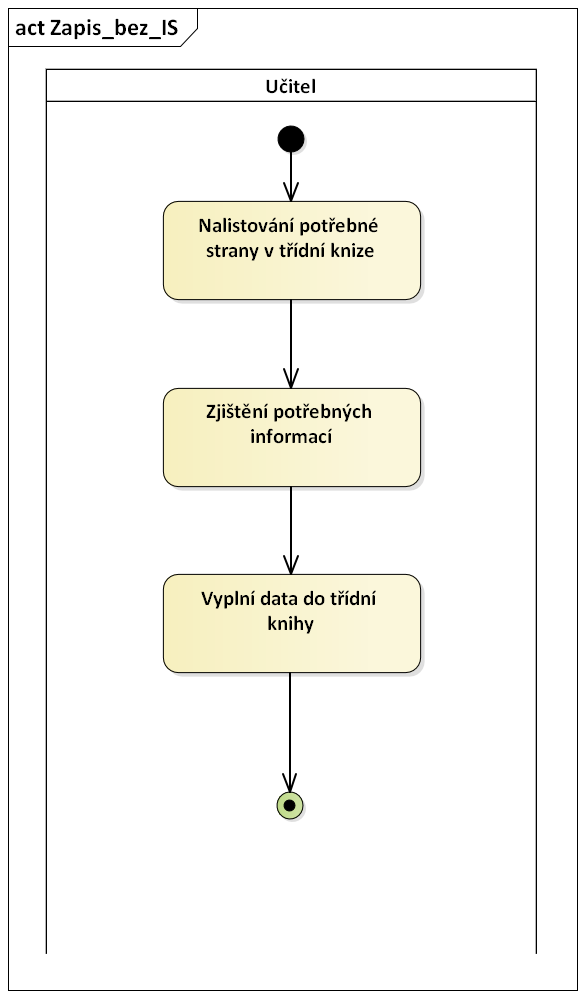
\includegraphics[width=0.5\textwidth]{images/Zapis_bez_IS.png}
	\caption{Proces zápisu o proběhnuté hodině bez informačního systému}
	\label{zapis_bez_IS}
\end{figure}

\subsubsection*{S použitím informačního systému}
S použitím informačního systému odpadá problém s hledáním zapomenuté třídní knihy. Další výhodou použití informačního systému také je přístup odkudkoliv, který pomáhá řešit problémy s třídní knihou vzniklé při distanční výuce.

Proces je stejně přímočarý, jako bez použití informačního systému. Učitel se nejdříve přihlásí do systému, vybere v aplikaci třídní knihu, do které chce zapisovat, zjistí informace a vyplní je. Vyplňovaná data jsou stejná, jako bez použití informačního systému. Všechny absence, které učitel zapíše, se automaticky dostávají do stavu \uv{neomluvená}.

\subsection{Omlouvání žáků}
\subsubsection*{Bez použití informačního systému}
Tento proces začíná u rodiče žáka. Ten napíše omluvenku do žákovské knížky nebo do omluvného listu a předá dokument svému dítěti. Dítě dokument přinese do školy a na začátku hodiny nebo o přestávce přijde k třídnímu učiteli a předává mu napsanou omluvenku. Třídní učitel omluvenku zkontroluje. Pokud je omluvenka v pořádku, nalistuje v třídní knize potřebnou stránku a omluví absenci žáka. Pokud omluvenka není v pořádku, vrací ji žákovi a ten pak tuto informaci směřuje zpět na svého zákonného zástupce, který musí napsat novou omluvenku.

V tomto procesu lze vidět několik problémů. Prvním problémem je, že je do tohoto procesu zapojen samotný žák, který může omluvenku zfalšovat. Není jisté, zdali rodič o absenci vůbec ví a jestli omluvenku psal on. Druhý problém je v tom, že omlouvání absence může zabírat čas na úkor výuky. Žáci nemají tendenci chodit s omluvenkou do kabinetu. Důvodem tohoto chování může být to, že třídní učitel nemusí mít k dispozici třídní knihu, ale také to, aby vědomě zkrátili čas vyučování.
Na obrázku \ref{omluva_bez_IS} lze vidět tento proces namodelovaný.
\clearpage

\begin{figure}[H]
	\centering
	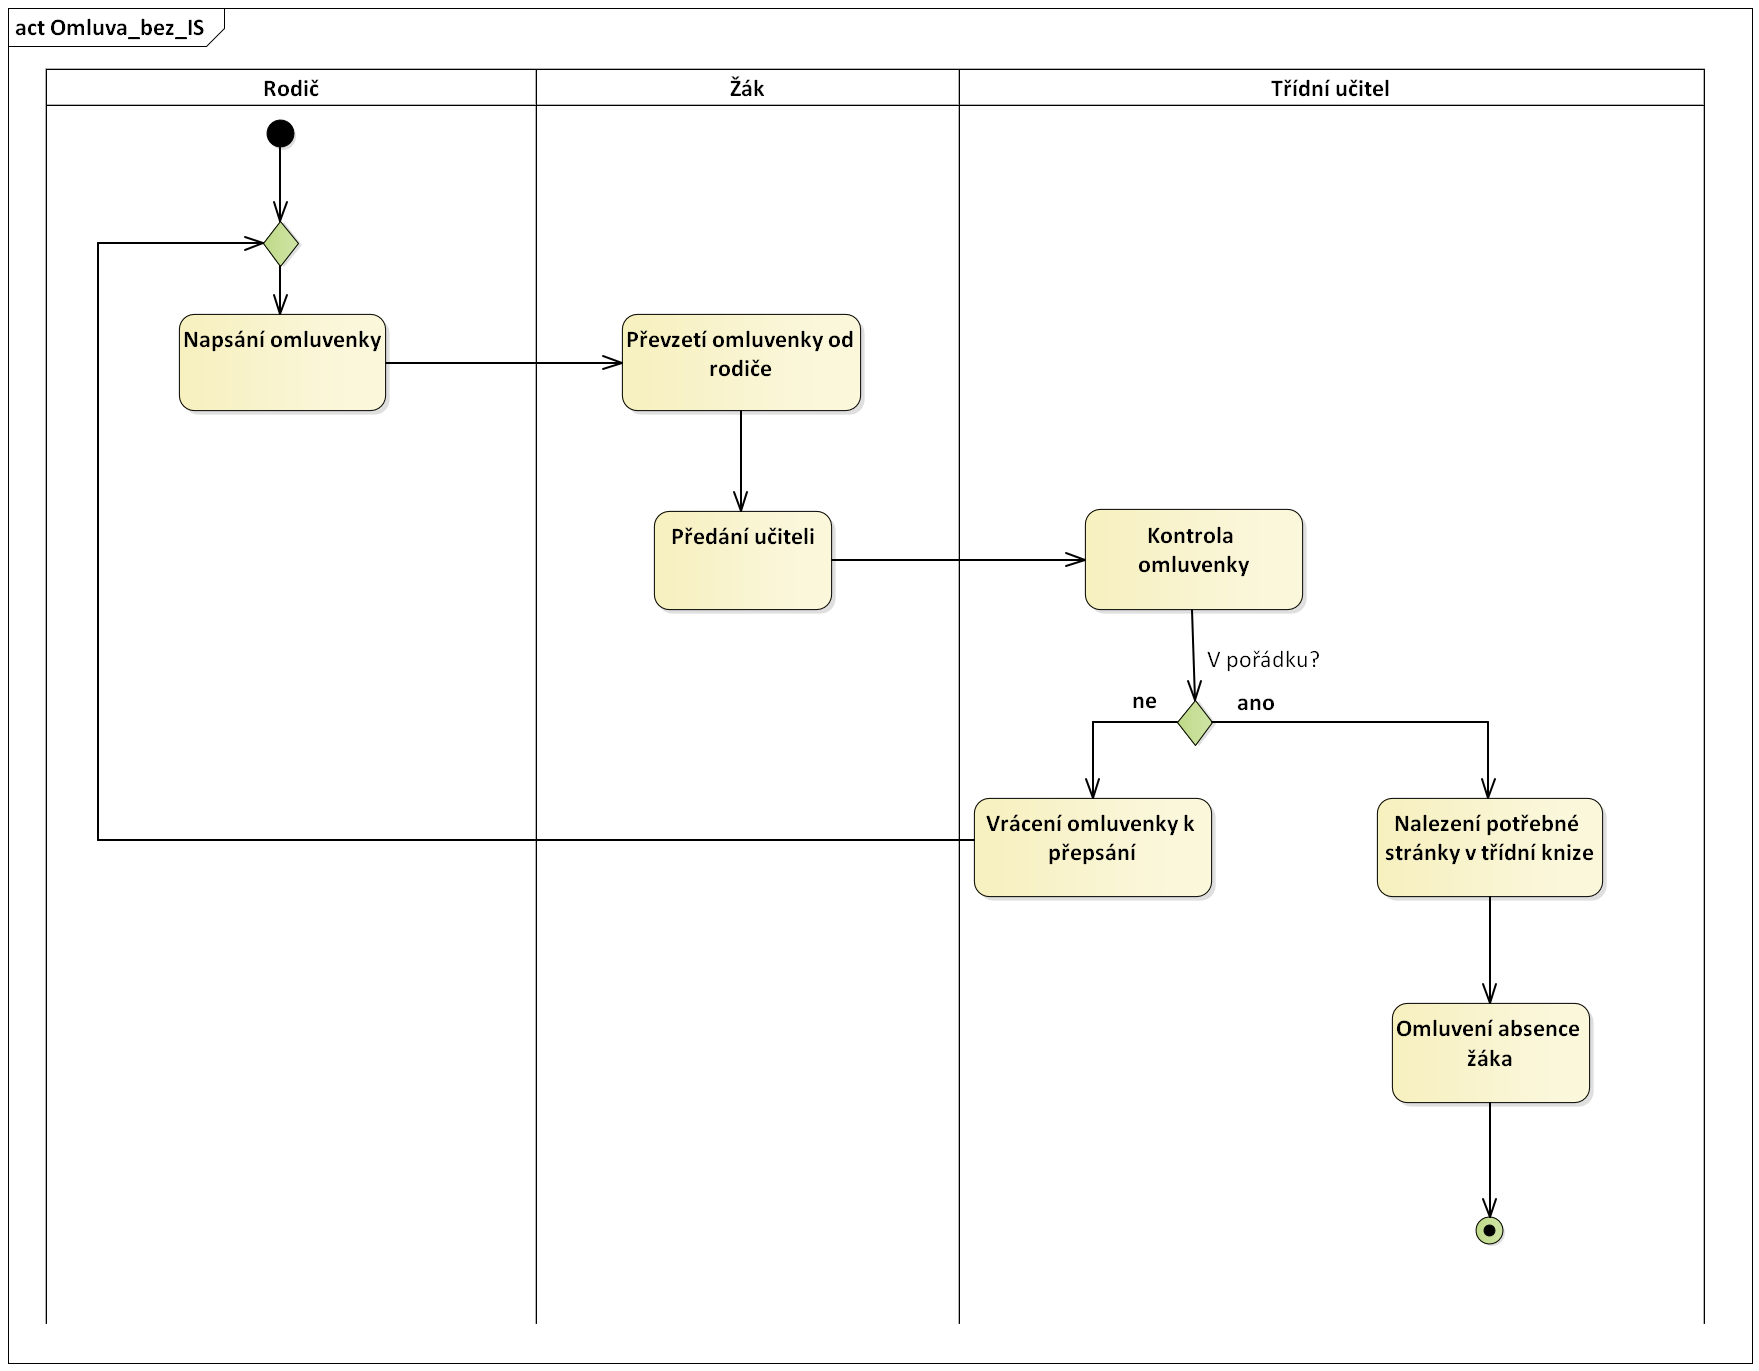
\includegraphics[width=\textwidth]{images/Omluva_bez_IS.png}
	\caption{Proces omlouvání žáků bez informačního systému}
	\label{omluva_bez_IS}
\end{figure}

\subsubsection*{S použitím informačního systému}
Proces s použitím informačního systému začíná opět u rodiče. Po přihlášení rodič vidí upozornění na novou absenci svého dítěte. Přepne se na stránku pro omluvu absencí, napíše zprávu a odešle. V tu chvíli se omluvenka dostává do stavu \uv{odeslána} a třídní učitel dostává upozornění o tom, že někdo poslal omluvenku. Následuje kontrola od třídního učitele. V případě, že je v pořádku, potvrdí omluvenku. Tím se omluvenka dostává do stavu \uv{potvrzena}. Systém poté absenci automaticky omluví a absenci přesune do stavu \uv{omluvená}. Pokud v pořádku není, omluvenku zamítne, čímž se dostává do stavu \uv{zamítnuta}. O zamítnuté omluvence dostane rodič upozornění a proces se opakuje.

Použitím informačního systému se odstranily všechny výše zmiňované problémy. Žák už do tohoto procesu vůbec nezasahuje a nemá tedy možnost omluvenku zfalšovat. Zároveň není možné zamlčet absenci, rodič vždy vidí absence svého dítěte. Vědomé zkracování času vyučování žákem je s použitím informačního systému také vyřešeno.
Tento proces lze vidět namodelovaný na obrázku \ref{omluva_s_IS}.
\clearpage

\begin{figure}[H]
	\centering
	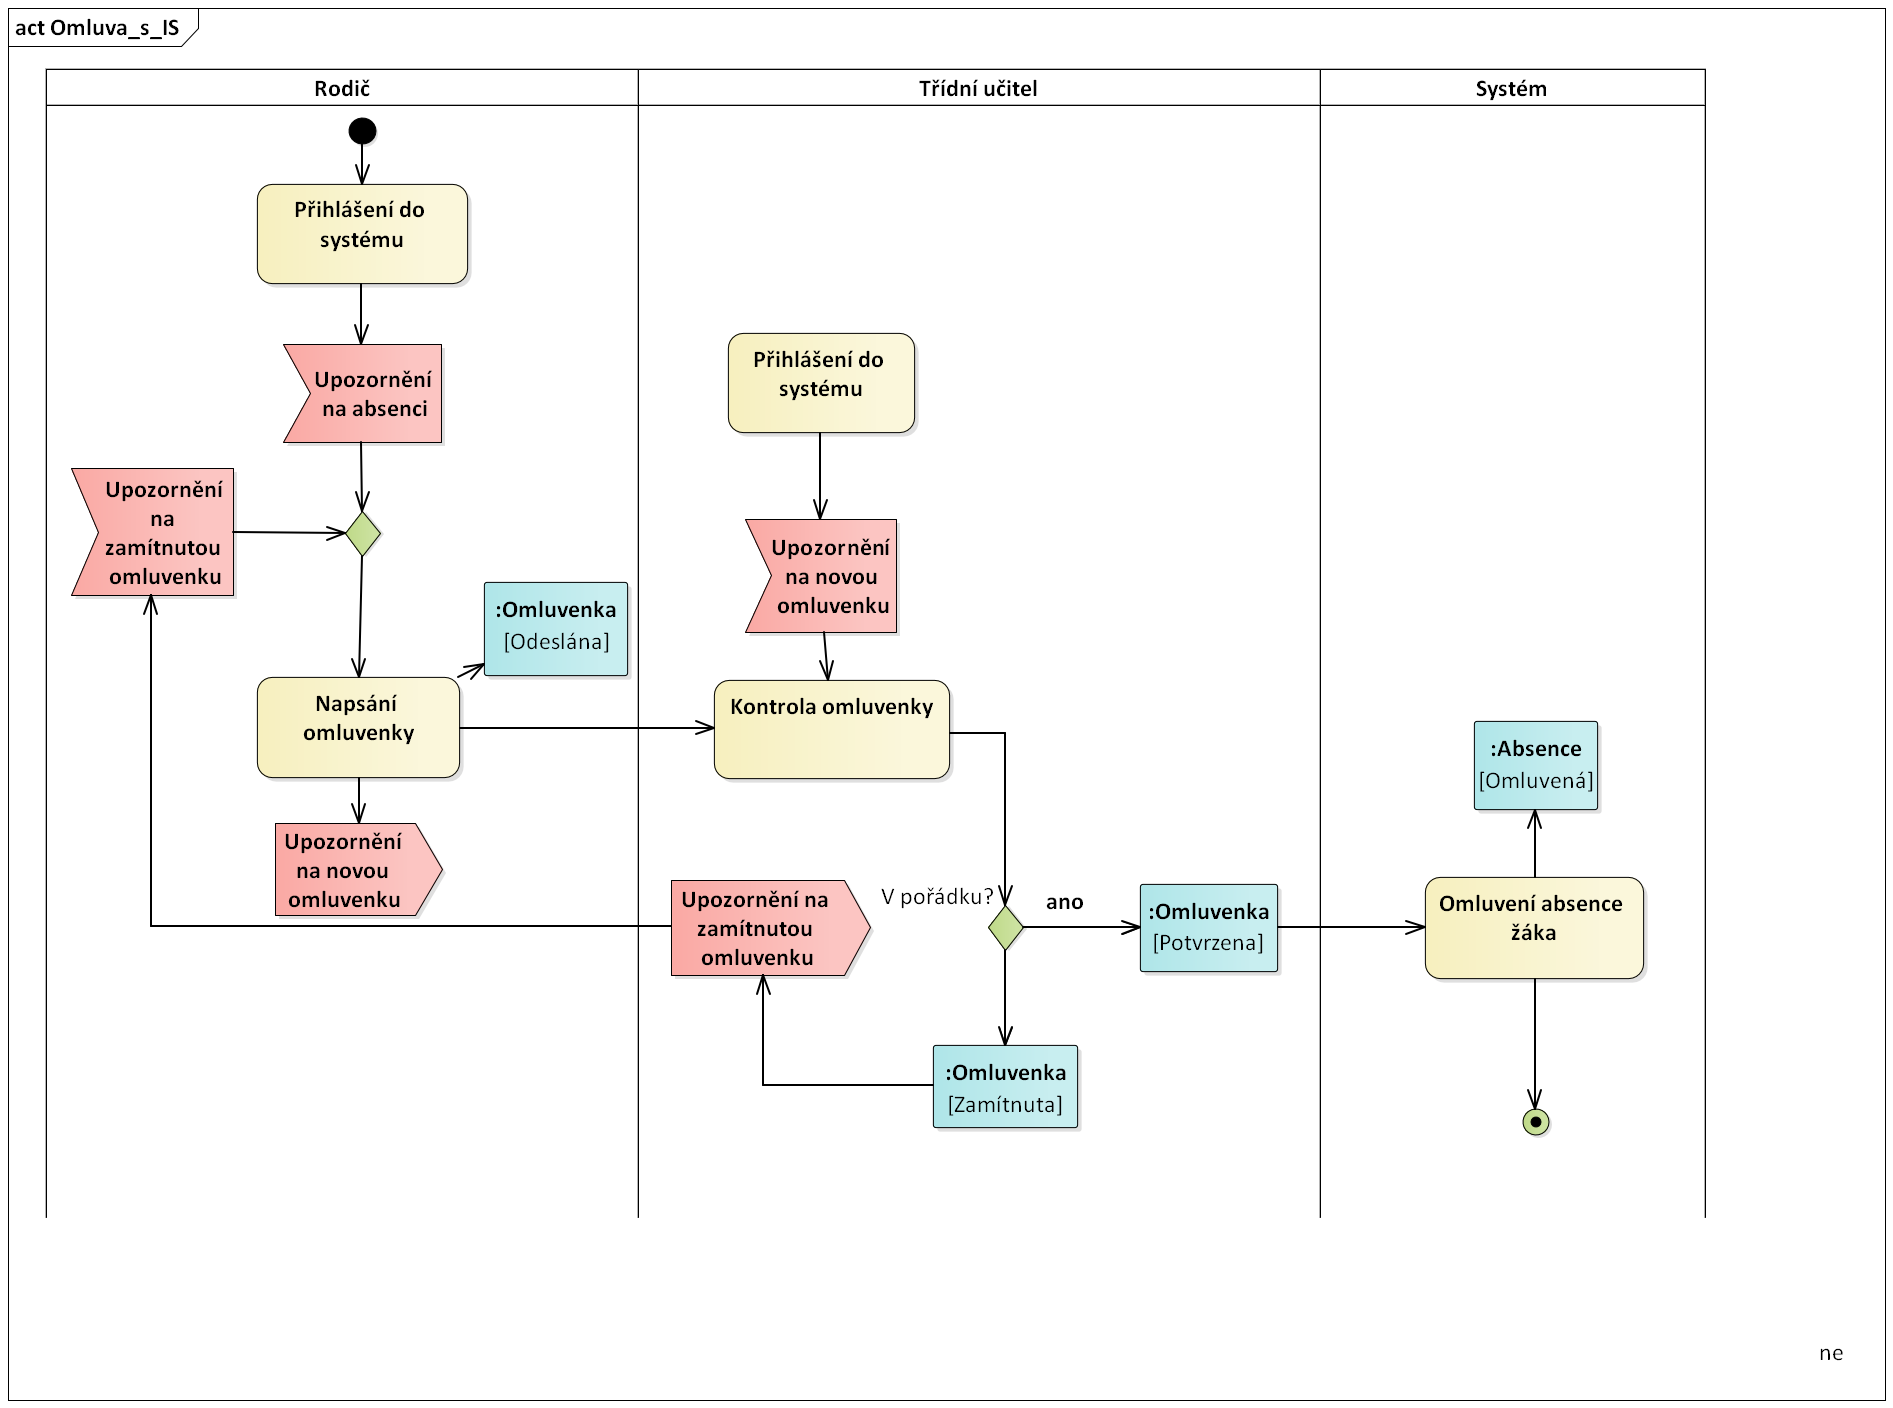
\includegraphics[width=\textwidth]{images/Omluva_s_IS.png}
	\caption{Proces omlouvání žáků s použitím informačního systému}
	\label{omluva_s_IS}
\end{figure}

\subsection{Obecné vytvoření události v hodině}
Zde je nejdříve potřeba si specifikovat, co se myslí událostí v hodině. Událost v hodině je hospitace, suplování, poučení nebo domácí úkol. Událost se vztahuje k určité hodině.
\subsubsection*{Bez použití informačního systému}
Proces je přímočarý. Učitel, zástupce ředitele nebo ředitel nalistuje potřebnou stránku v třídní knize a zapíše záznam o události. Namodelovaný proces je zobrazen na obrázku \ref{udalost_bez_IS}.
\clearpage

\begin{figure}[h]
	\centering
	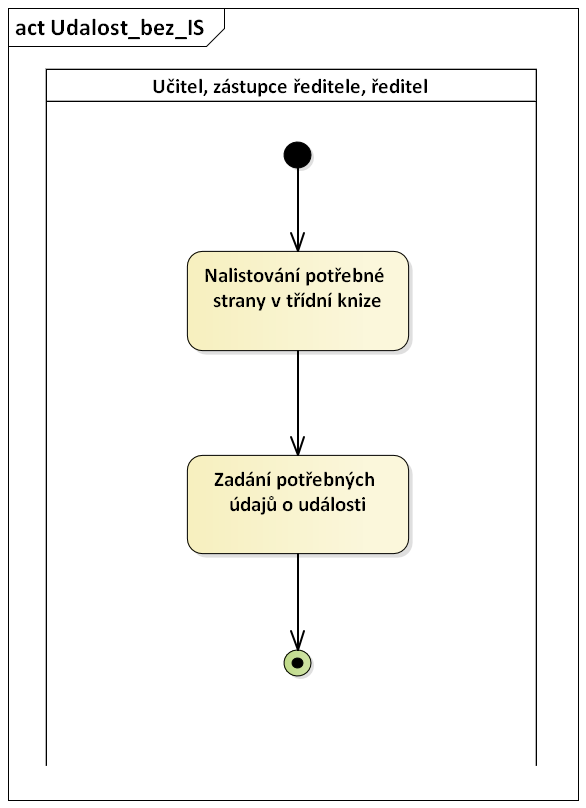
\includegraphics[width=0.5\textwidth]{images/Udalost_bez_IS.png}
	\caption{Proces vytvoření události bez informačního systému}
	\label{udalost_bez_IS}
\end{figure}

\subsubsection*{S použitím informačního systému}
Proces s použitím informačního systému je podobně přímočarý. Uživatel s rolí učitel, zástupce ředitele nebo ředitel se přihlásí do systému, vybere třídní knihu, u zvolené hodiny přidá událost a vyplní potřebné informace.

\subsection{Správa dat}
Tento proces již souvisí se správou dat v nově vytvořeném systému. Nedává smysl uvažovat nad tímto procesem bez informačního systému.

\subsubsection*{S použitím informačního systému}
Proces umožňuje spravovat data o uživatelích, předmětech, třídách, třídních knihách apod. Proces začíná přihlášením uživatele s rolí správce. Ten má možnost přepnout se do administrace systému. Vybere kategorii dat, kterou chce upravovat. Tam má možnost přidávat, odebírat či editovat jednotlivé záznamy.


\section{Doménový model}
Doménový model slouží k vizualizaci objektů reálného světa. Jeho cílem je popsat entity, vztahy mezi nimi a zachytit základní atributy entit. Třídy v doménovém modelu jsou značně zjednodušené a neobsahují žádné metody, pouze důležité atributy.

Doménový model popisující entity a vztahy v systému podporující správu třídních knih je zobrazen na obrázku \ref{domenovy_model}.

\begin{figure}[h]
	\centering
	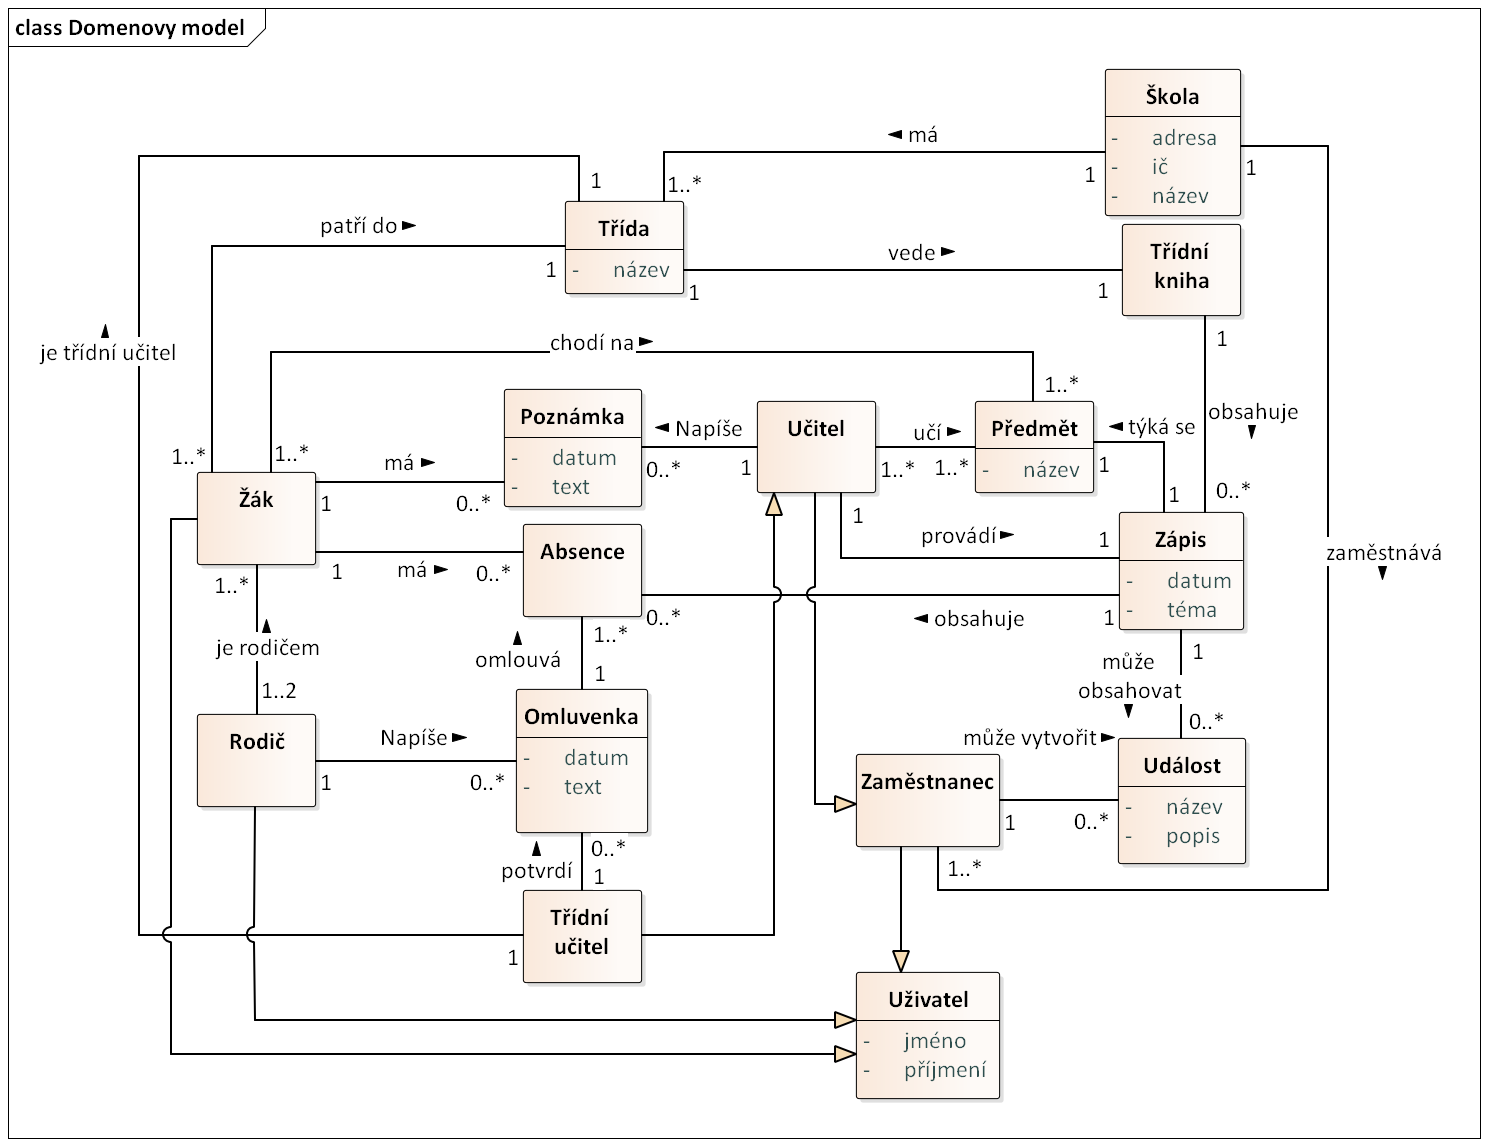
\includegraphics[width=\textwidth]{images/Domenovy_model.png}
	\caption{Doménový model}
	\label{domenovy_model}
\end{figure}

\subsection{Škola}
Třída \texttt{Škola} reprezentuje základní nebo střední školu. Hlavním atributem je název školy, adresa a identifikační číslo osoby (IČO).
\subsection{Třída}
Třída reprezentuje jednotlivé třídy ve škole. \texttt{Třída} má jednoho třídního učitele, jednu třídní knihu a několik žáků.
\subsection{Třídní kniha}
Každá třída je povinna vést třídní knihu. 
\subsection{Zápis}
Třída \texttt{Zápis} reprezentuje jednotlivé zápisy odučených hodin v třídní knize. Zápis se týká určitého předmětu, obsahuje téma a datum. Zápis souvisí s absencemi jednotlivých žáků a může obsahovat událost.
\subsection{Předmět}
Třída \texttt{Předmět} představuje jednotlivé předměty, které se ve škole učí. Předmět může být vyučován více učiteli.
\subsection{Událost}
Tato třída reprezentuje jednotlivé události, které se mohou danou hodinu konat. Jsou to například hospitace, poučení o bezpečnosti, suplování.
\subsection{Poznámka}
Jedná se o jednotlivé poznámky o chování žáků. Poznámku píše učitel určitému žákovi.
\subsection{Absence}
Tato třída představuje absence jednotlivých žáků. Absence musí být omluvena omluvenkou. Absence se vyplňují při zápisu do třídní knihy.

Tato třída má dva stavy. \uv{Neomluvená} a \uv{omluvená}. Při vytvoření absence se automaticky stává neomluvenou absencí. Stavy absence lze vidět na obrázku~\ref{stavy_absence}.

\begin{figure}[h]
	\centering
	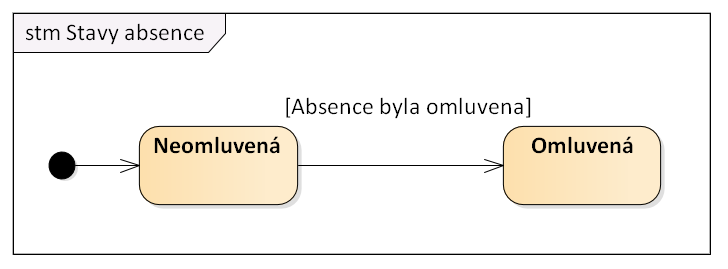
\includegraphics[width=0.75\textwidth]{images/Stavy_absence.png}
	\caption{Stavy absence}
	\label{stavy_absence}
\end{figure}

\subsection{Omluvenka}
Třída představuje omluvenky žáků. Všechny absence žáků musí být řádně omluveny. Omluvenku může napsat pouze rodič (zákonný zástupce) žáka nebo třídní učitel (pokud dostane omluvenku jiným způsobem). Omluvenka napsaná rodičem musí být potvrzena třídním učitelem.

Omluvenka má tři stavy. \uv{Odeslána}, \uv{potvrzena} a \uv{zamítnuta}. Namodelované stavy omluvenky lze vidět na obrázku \ref{stavy_omluvenky}.
\begin{figure}[h]
	\centering
	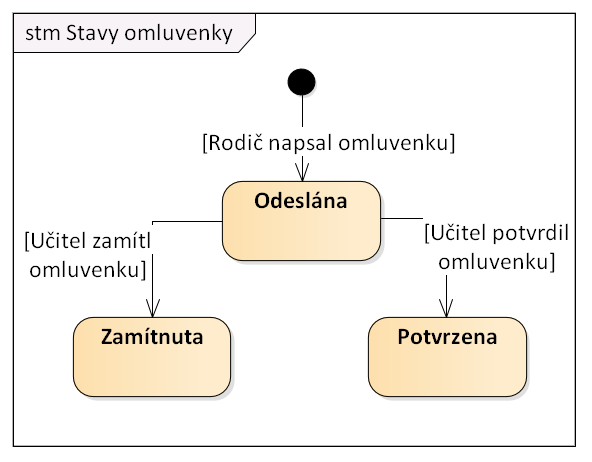
\includegraphics[width=0.6\textwidth]{images/Stavy_omluvenky.png}
	\caption{Stavy omluvenky}
	\label{stavy_omluvenky}
\end{figure}

\subsection{Učitel}
Jednotliví učitelé jsou reprezentováni touto třídou. Učitel je zaměstnán školou, vyučuje určité předměty, zapisuje do třídní knihy a může dávat jednotlivým žákům poznámky o jejich chování.
\subsection{Třídní učitel}
Speciální případ učitele. Má na starosti jednu třídu, u které vykonává činnosti třídního učitele. Jedna z těchto činností je starost o absence jednotlivých žáků. Třídní učitel potvrzuje omluvenky od rodičů žáka a může omluvenku napsat.
\subsection{Rodič}
Tato třída představuje jednoho rodiče (zákonného zástupce) žáka. Rodič může mít ve škole více než jednoho potomka. Žák má minimálně jednoho rodiče, maximálně však dva.
\subsection{Žák}
Třída \texttt{Žák} reprezentuje jednotlivé žáky ve škole, kteří jsou rozděleni do jednotlivých tříd. Žák chodí na určité předměty, může mít absence či poznámky.
\subsection{Zaměstnanec}
\texttt{Zaměstnanec} je nadtřídou pro učitele. Zaměstnanci mohou vytvářet jednotlivé události.
\subsection{Uživatel}
Třída \texttt{Uživatel} je nadtřídou všech možných uživatelů v systému.


\section{Funkční a nefunkční požadavky}
Tato podkapitola je věnována funkčním a nefunkčním požadavkům, které jsou kladeny na výsledný systém. Požadavky byly zpracovány na základě potřeb uživatelů. Tyto potřeby byly konzultovány s Mgr. Lenkou Tichou, která vyučuje na Základní škole Český Dub.

\subsection{Funkční požadavky}
Funkční požadavky jsou požadavky na chování systému. \cite{funkcni_pozadavky}

\subsubsection*{F1 Přihlášení do systému}
Uživatelé se mohou přihlašovat do systému. Registraci nemůže uživatel provést sám, do systému je musí přidat administrátor. Jednotliví uživatelé si mohou změnit heslo. V systému jsou uživatelé rozdělení do jednotlivých rolí:

\begin{itemize}
    \item Správce / administrátor
    \item Ředitel školy
    \item Zástupce ředitele
    \item Třídní učitel
    \item Učitel
    \item Žák
    \item Rodič
\end{itemize}

Jednotlivé role určují uživatelům možnosti, které jim systém poskytne. Jeden uživatel může mít nastaveno více rolí.

\subsubsection*{F2 Správa dat}
Systém bude umožňovat správu dat ve škole. Příkladem dat jsou informace o žácích, učitelích a rodičích, informace o předmětech, které se vyučují, seznam jednotlivých tříd. Tuto správu dat může provádět pouze uživatel s rolí správce.

\subsubsection*{F3 Zápis do třídní knihy}
Systém bude umožňovat uživatelům s rolí učitel zápis do třídní knihy. Učitel zapíše informace o hodině do třídní knihy. Informace, které lze zapsat, jsou absence žáků, předmět, kterého se zápis týká, téma a pořadové číslo hodiny v daný den.

\subsubsection*{F4 Omluva absence žáka}
Systém umožní omlouvat absence žáků. Každá absence žáka musí být řádně omluvena. K omluvení slouží omluvenka, která je napsána rodičem žáka nebo jeho třídním učitelem. V případě, že omluvenku napíše rodič, musí být následně potvrzena třídním učitelem.

\subsubsection*{F5 Vytvoření události v hodině}
V systému bude možné vytvářet v jednotlivých hodinách události. Událostí může být hospitace, suplování, poučení o bezpečnosti nebo domácí úkol. Událost hospitace může vytvořit pouze ředitel nebo zástupce ředitele. Událost domácí úkol a suplování může vytvořit pouze učitel. Poučení může vytvořit libovolný zaměstnanec.

\subsubsection*{F6 Přehledy}
V systému budou zobrazovány přehledy o žácích. Přehledy budou rozděleny podle rolí. 
Uživatel s rolí rodič vidí informace pouze o svých dětech. Žák vidí informace pouze o sobě. Učitelé, zástupce ředitele, ředitel a správci mají přehled o všech žácích.

Zobrazovány budou informace o žákově absenci, poznámkách, případně událostech v hodině (např. domácí úkoly).

\subsubsection*{F7 Archivace dat}
Systém musí umět skladované informace vyexportovat do formátu PDF a vytvořit tak třídní knihu, kterou lze archivovat. V tomto dokumentu musejí být informace o proběhnuté výuce, které byly do systému zapsány v určitém období, typicky za pololetí nebo celý školní rok.
Export do PDF může provádět uživatel s rolí správce, ředitel, zástupce ředitele a třídní učitel.


\subsection{Nefunkční požadavky}
Nefunkční požadavky určují omezení, která jsou kladena na systém. 
\subsubsection*{N1 Webová aplikace}
Systém bude vytvořen jako webová aplikace. Aplikace bude plně funkční pro webový prohlížeč Google Chrome 87.0.4280.88. 

\subsubsection*{N2 Responzivní design}
Design webové stránky bude responzivní, bude se přizpůsobovat velikosti okna, případně používanému zařízení.

\subsubsection*{N3 Snadná rozšiřitelnost systému}
Architektura systému bude navržena tak, aby případné budoucí rozšíření systému bylo co nejjednodušší.



\chapter{Rešerše existujících aplikací}
Tato kapitola se věnuje rešerši existujících aplikací, které se zaměřují na elektronizaci třídních knih. Na trhu existuje celá řada řešení. Vybrané aplikace zde budou podrobněji popsány, budou uvedeny klady a zápory jednotlivých systémů a bude provedeno jejich srovnání. Rešerše  bude zaměřena především na funkce systému, cenu, uživatelské rozhraní a podporu.

\section{Etřídnice}
Prvním vybraným řešením je aplikace Etřídnice \cite{etridnice}. Tu provozuje společnost just4web.cz s.r.o. a pro školní agendu ji využívá 75 400 uživatelů.

Tento školský informační systém je rozdělen do modulů, kde třídní kniha je jedním z nich. Dalším modulem je například žákovská knížka, rozvrh hodin, deník praxe a úkoly.

\subsection{Funkcionalita a rozhraní}
Modul třídní kniha plnohodnotně nahrazuje klasickou třídní knihu a obsahuje následující funkce: 

\begin{itemize}
    \item zápis předmětu a učiva,
    \item zápis absence žáků,
    \item hospitace a inspekce,
    \item zápis projektů,
    \item zápis akcí a kurzů,
    \item přehled zameškaných hodin (omluvených/neomluvených),
    \item přehled odučených hodin učitelů,
    \item tisk všech přehledů, jako v klasické třídní knize,
    \item přístup pro rodiče a žáky k absenci,
    \item možnost posílání e-mailu rodičům při absenci jejich dětí.
\end{itemize}

\noindent Uživatelské rozhraní je intuitivní a kvalitně zpracované. Na obrázku \ref{etridnice} lze vidět ukázku aplikace. Konkrétně zápis předmětu a učiva do třídní knihy. Aplikace se skládá z hlavičky, navigačního menu a hlavní sekce. V hlavičce se nachází informace o přihlášeném uživateli a vyhledávací lišta. V navigačním menu lze přepínat mezi jednotlivými moduly a funkcemi, i zde se nachází informace o uživateli. Hlavní sekce se mění podle vybrané funkce a probíhá v ní užitečná práce, např. zápis učiva, absence, hospitace, atd.

\begin{figure}[h]
	\centering
	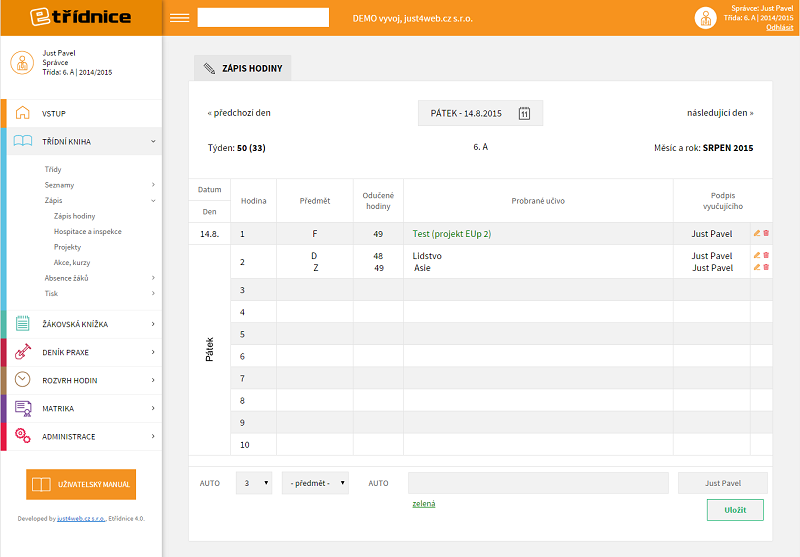
\includegraphics[width=\textwidth]{images/etridnice.png}
	\caption{Ukázka uživatelského rozhraní Etřídnice \cite{etridnice}}
	\label{etridnice}
\end{figure}

\subsection{Podmínky použití}
Cena se odvíjí od velikosti školy, respektive počtu žáků ve škole a platí se za roční licenci. Pohybuje se od 3~600 Kč pro počet žáků do 50, do 15~000~Kč, kde počet žáků může být až 1~000. V licenci jsou zahrnuty všechny moduly, včetně instalace a konfigurace systému, zálohování, aktualizací a uživatelské podpory. Ceny jsou uvedeny bez DPH. \cite{etridnice-cena} 

Systém Etřídnice je webová aplikace, jejíž hostování zajišťuje společnost just4web.cz s.r.o. Data, která aplikace ukládá, jsou umístěna na serveru poskytovatele, který je registrován u Úřadu pro ochranu osobních údajů. Pro přístup k nim se využívá protokol HTTPS, který se šifruje pomocí SSL. \cite{etridnice-podpora}

\subsection{Podpora}
Na webových stránkách Etřídnice nalezneme přehledný manuál k aplikaci. Ten je rozdělen na kapitoly, kde každému modulu je věnována právě jedna kapitola. Na stránkách najdeme i krátká videa, která demonstrují práci se systémem.

Společnost dále nabízí školení pro učitele či správce systému. Tato školení jsou však zpoplatněna. Cena za školení trvající dvě hodiny je 1 200 Kč.

\subsection{Identifikované klady a zápory}
Kladnými body řešení může být kvalitně zpracované uživatelské rozhraní, přehledný manuál a nižší cena oproti konkurenční aplikaci Edookit.

Naopak zápornými body může být nutnost uložení dat u poskytovatele a také fakt, že systém je sice rozdělen na moduly, ale licence, kterou je nutné zakoupit, obsahuje vždy všechny moduly. Není tedy možné vybrat si pouze určitý výčet modulů a platit například nižší cenu za licenci.

\section{Bakaláři}
Nejrozšířenější řešení v ČR je systém Bakaláři od společnosti BAKALÁŘI software s.r.o. \cite{bakalari}. Tento program používá přes milion uživatelů v ČR \cite{bakalari}. Stejně jako předchozí systém je i tento logicky rozdělen na moduly. Třídní kniha je jedním z modulů. Dalšími moduly, které řešení obsahuje, jsou například žákovská knížka, evidence žáků a zaměstnanců či modul pro přijímací zkoušky, knihovnu a inventarizaci.

\subsection{Funkcionalita a rozhraní}
Modul pro správu třídních knih plně nahrazuje třídní knihy v papírové podobě. V tomto modulu najdeme následující funkce:

\begin{itemize}
    \item zápis jednotlivých hodin,
    \item zápis nepřítomnosti žáků,
    \item omlouvání absence třídním učitelem,
    \item tiskové výstupy,
    \item poznámky o zadání domácího úkolu,
    \item zobrazení pořádkové služby,
    \item hospitace,
    \item poučení o bezpečnosti práce,
    \item specifická data žáků -- např. informaci o tom, že dojíždí,
    \item kontrola zapsaných hodin -- např. před archivací zkontrolovat, zdali něco nechybí,
    \item kontrola absencí.
\end{itemize}

\noindent Společnost nabízí pro přístup do systému tři řešení. Jedná se o desktopovou aplikaci, která je nainstalována na počítačích ve škole, webovou aplikaci a mobilní aplikaci.

Obrázek \ref{bakalari1} zobrazuje ukázku desktopové aplikace. Uživatelské rozhraní není moderní ani uživatelsky přívětivé. Zápis do třídní knihy probíhá přes nové okno, kde se vyplní téma hodiny, absence žáků apod. Informace o hodině se vyplní automaticky díky modulu rozvrhu a suplování. Bez tohoto modulu společnost nedoporučuje používat modul pro třídní knihu.

\begin{figure}[H]
	\centering
	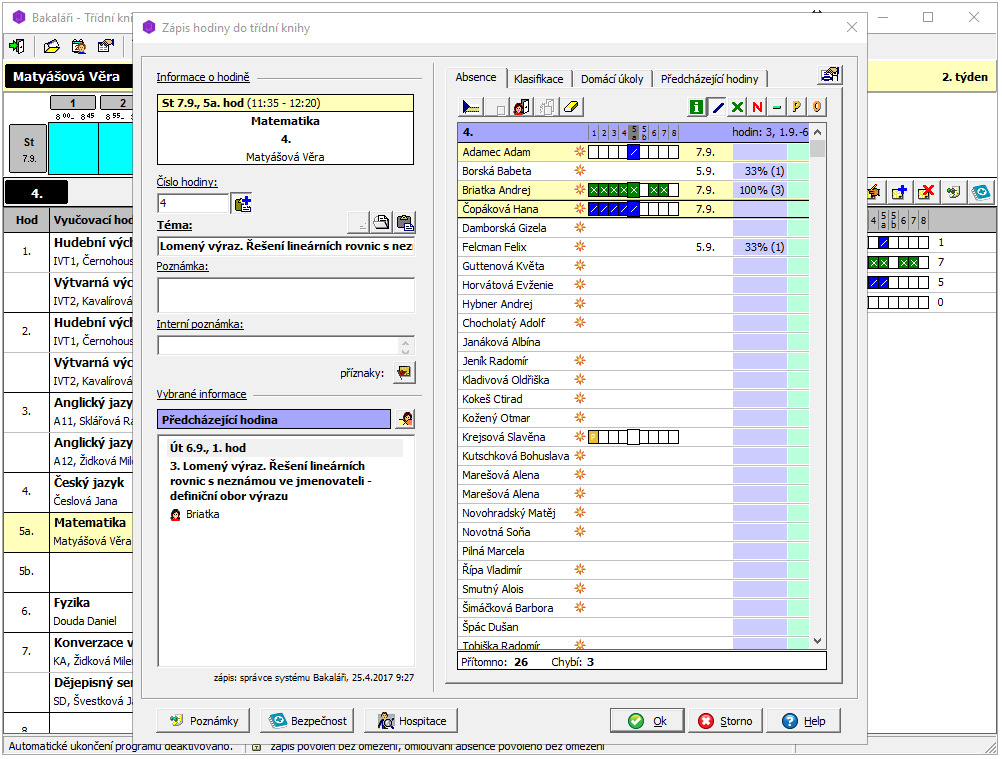
\includegraphics[width=\textwidth]{images/bakalari1.png}
	\caption{Desktopová aplikace systému Bakaláři \cite{bakalari}}
	\label{bakalari1}
\end{figure}

Na obrázku \ref{bakalari2} lze vidět ukázku webové aplikace Bakaláři. V tomto případě je uživatelské rozhraní již přívětivější. Aplikace je rozdělena na tři části. Hlavičku, která je umístěná nahoře a obsahuje informace o přihlášeném uživateli. Navigační menu, umístěné na levé straně aplikace, které slouží k přepínání na jednotlivé funkce. Hlavní část, kde probíhá užitečná práce se systémem.

\begin{figure}[h]
	\centering
	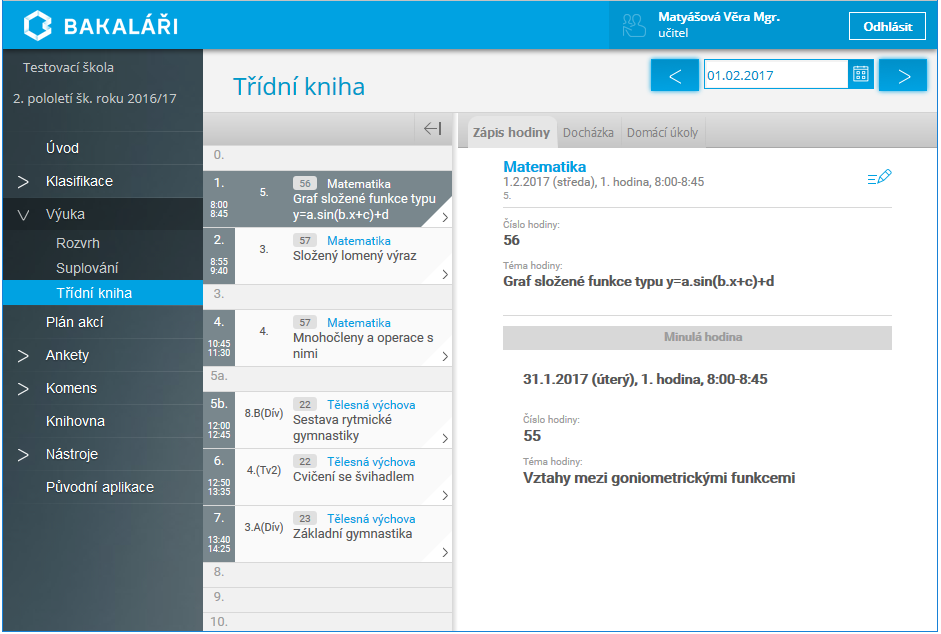
\includegraphics[width=\textwidth]{images/bakalari2.png}
	\caption{Webová aplikace systému Bakaláři}
	\label{bakalari2}
\end{figure}


\subsection{Podmínky použití}
Cena se stejně jako u předchozího systému odvíjí od velikosti školy a platí se za roční pronájem licence. Je možnost zakoupit pouze některé moduly, není tedy nutnost kupovat všechny. Přesná cena, či rozsah není zveřejněn.

Společnost BAKALÁŘI software s.r.o. umožňuje tři způsoby provozu aplikace. 
První možnost je provoz ve školní síti. Zde je aplikace provozována na virtuálním nebo fyzickém serveru školy. Výhoda tohoto řešení je především to, že vše je uloženo ve škole. Nevýhodou je nutnost pořídit server a licenci pro MS Server a nutnost udržovat provoz serveru. \cite{bakalari_nasazeni}

Druhá možnost je provozovat systém plně v cloudu poskytovatele. Výhodou u tohoto způsobu je, že není nutné pořizovat server ani licenci, vše je v režii poskytovatele. Nevýhodou může být svěření dat poskytovateli, měsíční platby za cloud či nutnost internetu k přístupu do systému. \cite{bakalari_nasazeni}

Poslední možností je kombinace dvou předchozích. V tomto případě je systém Bakaláři nainstalován na souborovém serveru školy, webová aplikace a data jsou pak v cloudu poskytovatele. Hlavní výhodou je, že webová aplikace běží nezávisle na škole, případný výpadek konektivity ve škole neovlivní přístup rodičů a žáků. Další výhodou je, že není nutné vlastnit a provozovat fyzický server s MS Server operačním systémem. Nevýhodou jsou opět měsíční poplatky za cloud, data u poskytovatele a nutnost internetového připojení pro provoz. \cite{bakalari_nasazeni}

\subsection{Podpora}
Společnost poskytuje návod na obsluhu systému na svých webových stránkách a krátká videa demonstrující některé funkcionality na platformě YouTube.

Co se týče technické podpory, společnost nabízí mailovou podporu bez analýzy dat a telefonickou podporu v pracovní době bez připojení přes vzdálenou plochu zdarma. Další služby jsou již zpoplatněny a jsou rozděleny do tří skupin. Jedná se o standardní služby, kam patří například analýza problému ze zaslaných dat či obnova dat ze zálohy. Zde je hodinová sazba nastavena na 1 200 Kč/hod. Pokud se však zjistí, že problém nevznikl na straně školy, jsou i tyto služby zdarma. Druhá skupina jsou individuální služby. Ty se objednávají až měsíc dopředu a cena je dohodnutá předem při objednávce a posouzení složitosti zásahu. Mezi tyto služby patří například převod dat z jiných systémů či tvorba rozvrhu na zakázku. Třetí skupinou je tzv. služba PODPORA+. Jedná se o doplňkovou službu k zakoupené licenci v podobě nadstandardní technické podpory. Jedná se například o přednostní odbavení telefonních hovorů, vzdálenou podporu TeamViewer či instalaci SQL serveru.

Veškerou placenou podporu zajišťují buď pracovníci společnosti Bakaláři software s.r.o. nebo certifikovaní konzultanti.

\subsection{Identifikované klady a zápory}
U řešení Bakaláři může být kladným bodem možnost vybrat si, kde bude aplikace provozována a kde budou uložena data. Další výhodou může být rozdělení do modulů podle funkcionalit a kvalitní podpora. V tomto případě lze zakoupit pouze určitý výčet modulů.

Nevýhodou je špatně zpracované uživatelské rozhraní u desktopové aplikace. Cena systému není zveřejněna, což znemožňuje tvořit v tomto směru objektivní závěr.

\section{Edookit}
Řešení Edookit od stejnojmenné firmy Edookit s.r.o. je kompletní informační systém pro mateřské, základní, střední a vyšší odborné školy \cite{edookit}. Tuto aplikaci využívá 350 000 aktivních uživatelů. Systém běží v cloudu a obsahuje funkcionalitu pro třídní knihu, žákovskou knížku, matriku, tvorbu rozvrhu, administrativu školy a komunikaci se studenty, rodiči a kolegy. 

\subsection{Funkcionalita a rozhraní}
Elektronická třídní kniha v tomto řešení umožňuje:

\begin{itemize}
    \item zapisovat a omlouvat absenci žáků,
    \item zapisovat probrané učivo,
    \item vkládat úkoly na příští hodinu,
    \item mít seznam žáků ve třídě nebo předmětu a jejich zasedací pořádek,
    \item vytvářet či měnit tematické plány,
    \item hodnotit žáky pomocí známek, procent či slovním hodnocením,
    \item sestavovat multimediální obsah z textu, obrázku, online testů, apod.,
    \item sdílet informace s vybranými skupinami či jednotlivci.
\end{itemize}

Aplikace je přístupná jak z webového prohlížeče, tak z mobilní aplikace. Uživatelské rozhraní je přehledné a intuitivní. Na obrázku \ref{edookit} lze vidět rozhraní aplikace Edookit. Aplikace se skládá z hlavičky nahoře, kde jsou odkazy na hlavní části aplikace a informace o přihlášeném uživateli, a z hlavní sekce, kde nahoře jsou odkazy na jednotlivé funkcionality a pod nimi již samotný obsah aplikace.

\begin{figure}[h]
	\centering
	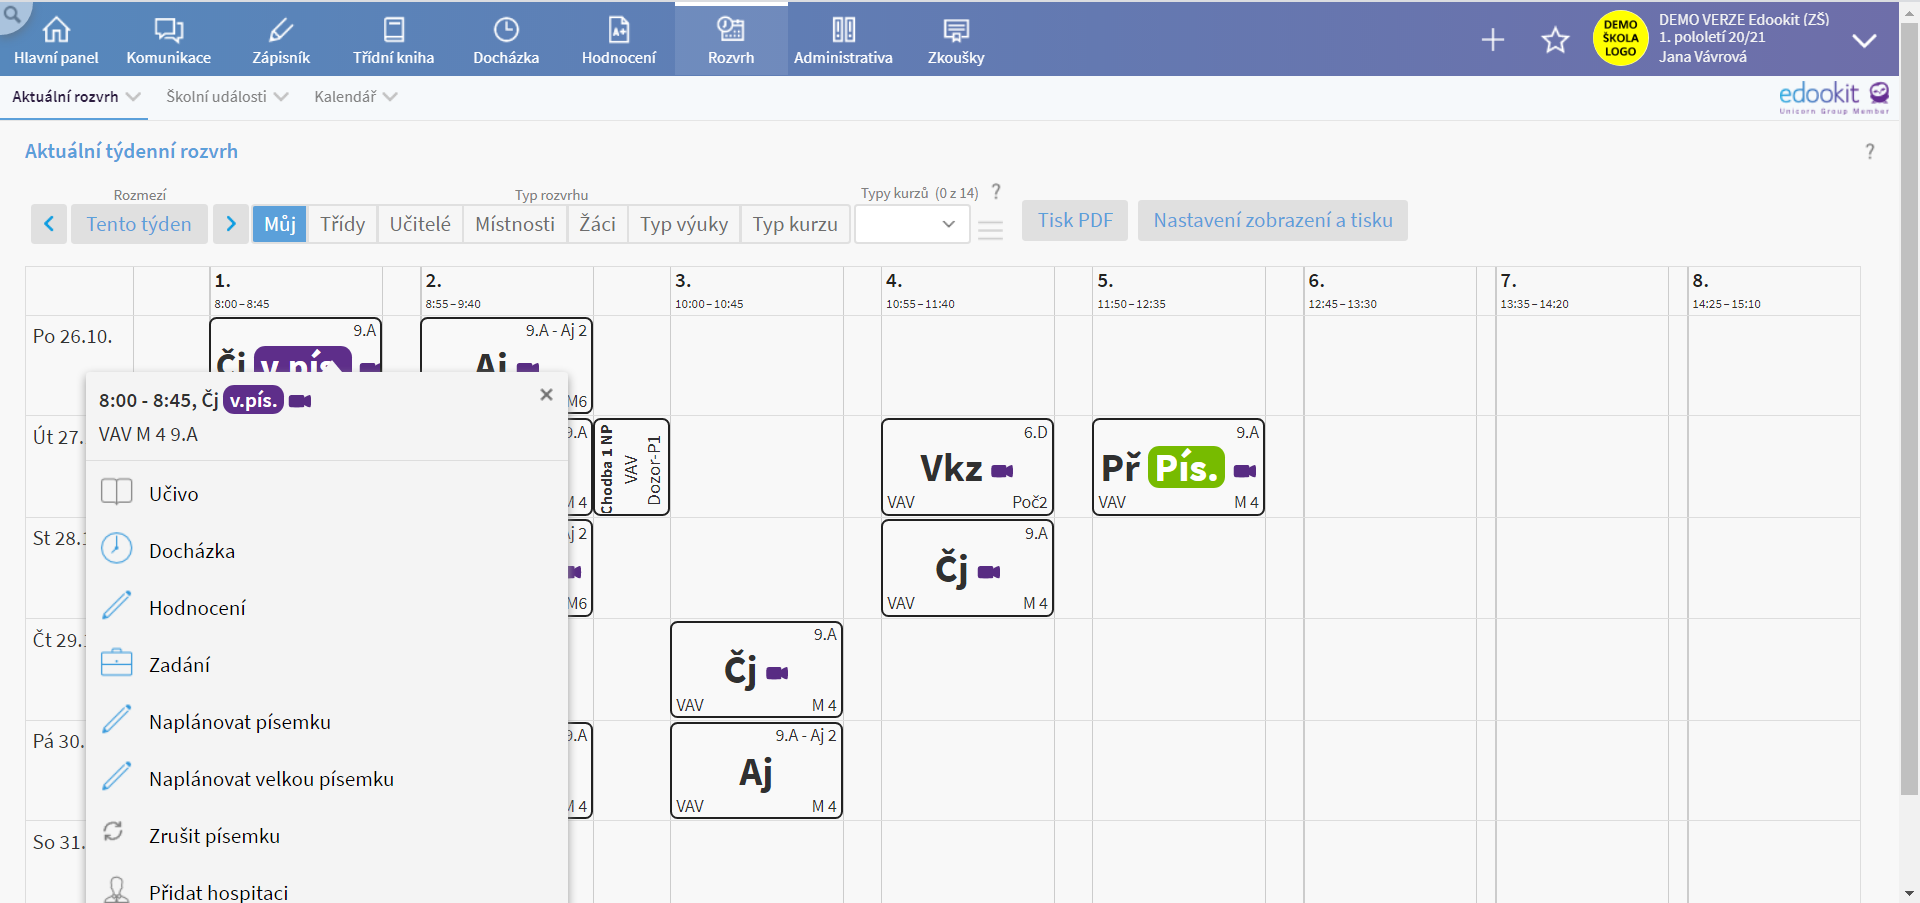
\includegraphics[width=\textwidth]{images/edookit.png}
	\caption{Ukázka uživatelského prostředí Edookit \cite{edookit}}
	\label{edookit}
\end{figure}

\subsection{Podmínky použití}
Systém není cenově rozdělen na moduly, cena zahrnuje celý informační systém. Cena se i zde odvíjí od velikosti školy, resp. počtu žáků a platí se za roční provoz. Pro mateřské, základní a střední školy se cena pohybuje od 14 400~Kč pro počet žáků do 100, do 79 900 Kč pro počet žáků do 1 000. Pro vyšší odborné školy je cena vyšší. Pohybuje se od 24 000 Kč pro počet studentů do 100, do 187 200 Kč pro počet studentů menší než 1 000. Cena je uvedena včetně DPH 21\% a zahrnuje provoz aplikace, aktualizace, datový prostor 100~GB, technickou podporu a zálohování. Instalační poplatek zahrnující vložení školy do systému, import dat, počáteční nastavení a úvodní školení pro učitele je stanoven na 3 000 Kč vč. DPH.

Edookit je webová aplikace, jejíž hostování zařizuje společnost Edookit s.r.o. Podle obchodních podmínek \cite{edookit-podminky} jsou data \uv{\textit{ukládána a spravována v souladu s Nařízením Evropského parlamentu a Rady (EU) 2016/679 o ochraně fyzických osob v souvislosti se zpracováním osobních údajů a o volném pohybu těchto údajů a o zrušení směrnice 95/46/ES (obecné nařízení o ochraně osobních údajů, dále jen Nařízení GDPR)}}.

\subsection{Podpora}
Společnost na svých webových stránkách poskytuje návody ve formě PDF pro jednotlivé funkce a úkony. Mají také zveřejněnou nahrávku ze školení pro učitele. Dále nabízejí zpoplatněné služby jako například navýšení datového prostoru, nadstandardní školení či vývoj speciální nové funkce. Na webových stránkách poskytují odkaz na demo verzi, kde je možné systém zdarma vyzkoušet.

\subsection{Identifikované klady a zápory}
U řešení Edookit jsou kladným bodem kvalitně zpracované návody.

Nedostatkem tohoto řešení je především absence rozdělení funkcionalit na moduly, což znamená, že škola musí platit za celý systém, i když chce využívat například jen zlomek funkcionalit. Další nevýhodou je cena, která je oproti konkurenčnímu řešení Etřídnice vyšší. Pro některé školy může být také překážka to, že data musí být uložena pouze u poskytovatele a ne na školním serveru. Poslední nalezenou nevýhodou může být uživatelské rozhraní, které není z pohledu autora této práce příliš intuitivní a je potřeba si nastudovat uživatelskou příručku. 

\section{Srovnání}
V této kapitole byla provedena rešerše třech systémů, které řeší problém elektronizace třídních knih. Všechna zkoumaná řešení mají své silné a slabé stránky, které jsou uvedeny v jednotlivých podkapitolách. Ať už si škola vybere jakýkoliv zmíněný systém, nevyhne se kompromisům. Těmi mohou být například:

\begin{itemize}
    \item uživatelské rozhraní (Bakaláři, Edookit),
    \item nutnost pořídit celý systém, ne pouze výčet modulů (Etřídnice, Edookit),
    \item data uložená pouze u poskytovatele (Etřídnice, Edookit),
    \item cena (Edookit).
\end{itemize}

\noindent Všechny aplikace nabízejí víceméně stejnou základní funkcionalitu pro správu třídních knih. Rozdíly jsou především v uživatelském rozhraní, provozu aplikace a cenové politice.

Funkcionalita je u všech řešení logicky rozdělena do funkčních celků, kde třídní kniha je jednou z nich. Dále nabízejí žákovské knížky, matriku, rozvrhy, přístup pro rodiče a další. Řešení Bakaláři nabízí modul pro přijímací zkoušky a inventarizaci, což konkurenční aplikace nenabízí.

Uživatelské rozhraní je dalším rozdílem uvedených systémů. Kvalitně zpracovaným uživatelským rozhraním, které je zároveň intuitivní, disponuje aplikace Etřídnice. Naopak u aplikací Edookit a Bakaláři je intuitivnost rozhraní menší.

Další rozdíly lze vidět i v provozu systému. Zde vyniká řešení Bakaláři, které nabízí tři druhy provozu -- ve školní síti, v cloudu poskytovatele a kombinaci předchozích dvou. Oproti tomu aplikace Edookit a Etřídnice nabízí pouze provoz u poskytovatele.

Poslední rozdíl je v cenové politice společností. U systémů Etřídnice a Edookit nelze platit pouze za výčet funkcionalit systému a je potřeba si pořídit celý systém. Řešení Bakaláři se v tomto ohledu odlišuje, zde společnost nabízí možnost platit pouze za některé moduly.
Konkrétní ceny jsou zveřejněné pouze u systémů Etřídnice a Edookit. Zde je levnější řešení Etřídnice, kde se za roční licenci platí 3 600 -- 15 000 Kč bez DPH. U řešení Edookit se roční cena pohybuje mezi 11 900 -- 154 710 Kč bez DPH.


\chapter{Návrh}
Tato kapitola je věnována návrhu informačního systému pro správu třídních knih. V prvé řadě budou vytvořeny případy užití, tedy průchody budoucí aplikací. Ty představují návrh toho, jak bude systém naplňovat funkční požadavky, které byly definovány v předchozí kapitole určené analýze. Dále bude věnován prostor architektonickému návrhu systému. Zde bude zvolena vhodná architektura, která bude použita při implementaci aplikace. Poslední část kapitoly bude věnována návrhu uživatelského rozhraní několika základních obrazovek.

\section{Model případů užití}
Model případů užití slouží k detailní specifikaci funkčních požadavků. Navrhují se průchody budoucí aplikací. Typicky obsahuje seznam účastníků, diagram případů užití a jejich popis. Slouží jako zadání pro programátora, tvorbu akceptačních testů či tvorbě uživatelské příručky. \cite{pripady-uziti-prednaska}
\clearpage
\subsection{Účastníci}
Obrázek \ref{ucastnici} zobrazuje uživatele systému. Účastníci jsou použiti jako aktéři v případech užití.

\begin{figure}[h]
	\centering
	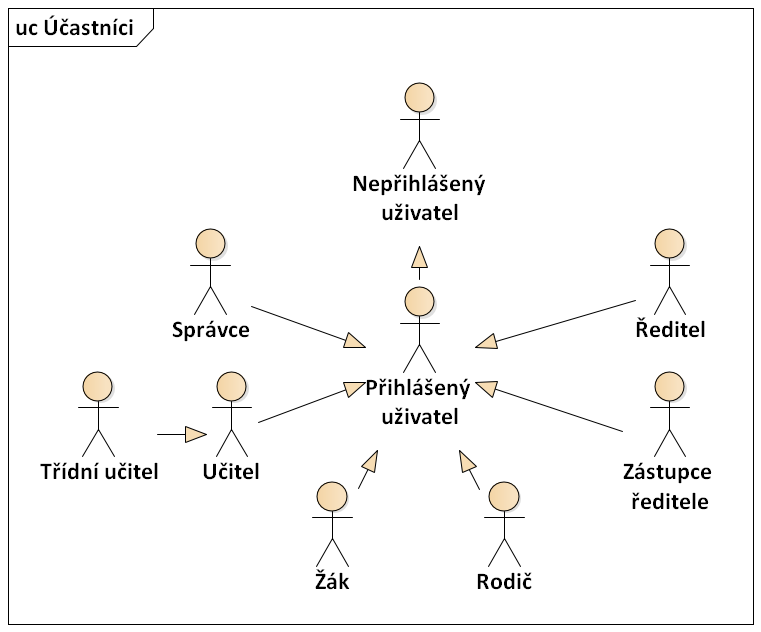
\includegraphics[width=\textwidth]{images/ucastnici.png}
	\caption{Aktéři případů užití}
	\label{ucastnici}
\end{figure}

\clearpage
\subsection{Případy užití}
\subsubsection{Obecné}
Na obrázku \ref{pripady-obecne} lze vidět namodelované obecné případy užití.

\begin{figure}[h]
	\centering
	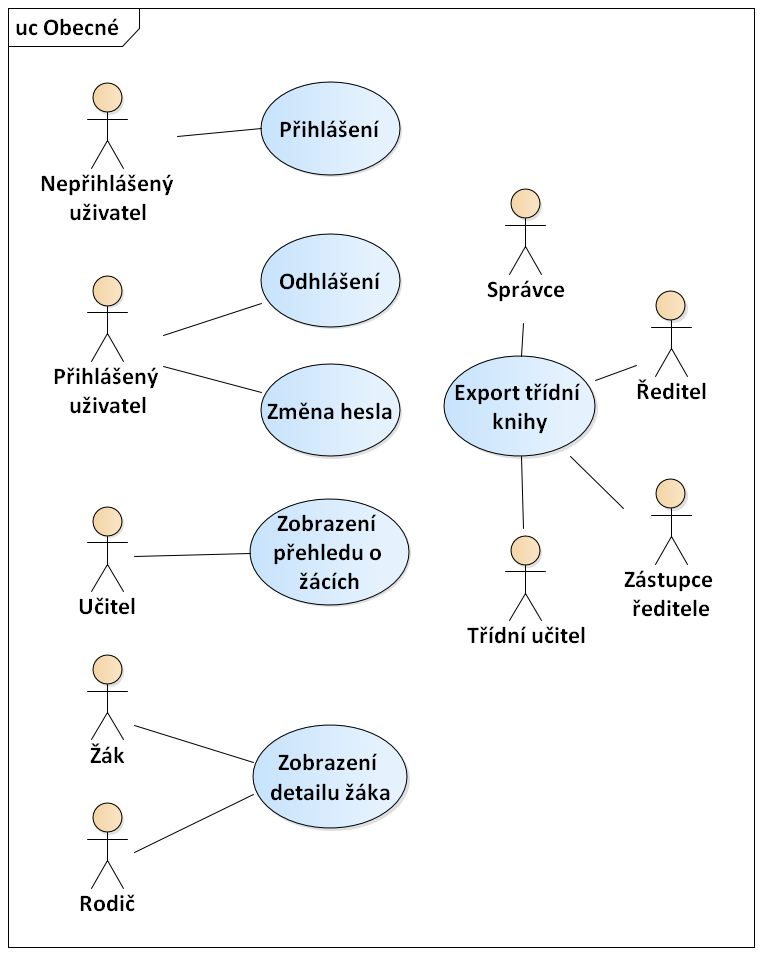
\includegraphics[width=\textwidth]{images/obecne.png}
	\caption{Obecné případy užití}
	\label{pripady-obecne}
\end{figure}

\subsubsection*{UC1 Přihlášení}
Umožňuje nepřihlášenému uživateli přihlášení do systému. 
\begin{itemize}
    \item Uživatel vyplní e-mail a heslo a klikne na tlačítko \uv{Přihlásit}, čímž se přihlásí do systému.
\end{itemize}

\subsubsection*{UC2 Změna hesla}
Umožňuje uživateli změnit přístupové heslo.
\paragraph{Hlavní scénář}
\begin{itemize}
    \item Uživatel se přihlásí do systému.
    \item Rozklikne ovládací menu a zvolí položku \uv{Účet}.
    \item Klikne na tlačítko pro změnu hesla.
    \item Dostane se na formulář pro změnu hesla, kde zadá stávající heslo, nové heslo a potvrzení nového hesla. Po potvrzení formuláře se heslo změní.
\end{itemize}

\paragraph{Alternativní scénář}
\begin{itemize}
    \item Nepřihlášený uživatel na přihlašovací obrazovce stiskne tlačítko pro zapomenuté heslo, čímž se dostane na formulář pro obnovu hesla.
    \item Ve formuláři zadá e-mailovou adresu, kterou se přihlašuje do systému.
    \item Na zadaný e-mail mu přijde odkaz, který ho přesměruje na formulář pro zadání nového hesla. 
    \item Ve formuláři vyplní nové heslo a potvrzení nového hesla. Po potvrzení formuláře se heslo změní.
\end{itemize}

\subsubsection*{UC3 Odhlášení}
Umožňuje odhlášení uživatele ze systému.

\subsubsection*{UC4 Export třídní knihy}
Umožňuje uživateli s rolí správce, ředitele, zástupce ředitele nebo třídního učitele vyexportovat třídní knihu do souboru PDF.
\begin{itemize}
    \item Uživatel s požadovanou rolí se přihlásí do systému.
    \item V navigačním menu si vybere políčko, které mu ukáže seznam třídních knih.
    \item U položky, která odkazuje na danou třídní knihu klikne na tlačítko pro export třídní knihy.
    \item Tím se dostane na formulář, kde zadá časový rozsah, ve kterém chce třídní knihu tisknout.
    \item Potvrzením formuláře vygeneruje systém PDF soubor s třídní knihou.
\end{itemize}

\subsubsection*{UC5 Zobrazení přehledu o žácích}
Umožňuje uživatelům s příslušnou rolí zobrazit si seznam žáků s jejich přehledem. Přehled si mohou zobrazit uživatelé s rolí učitel, ředitel, zástupce ředitele a správce.
\begin{itemize}
    \item Uživatel se přihlásí do systému.
    \item V navigačním menu se přepne do sekce s přehledy.
    \item Po výběru třídy z nabídky se uživateli zobrazí seznam žáků v dané třídě.
    \item U každého žáka v seznamu je možné přejít na jeho detail.
\end{itemize}

\subsubsection*{UC6 Zobrazení detailu žáka}
Umožňuje zobrazit informace o žákovi. Bude zobrazovat informace o absenci, poznámkách či domácích úkolech. Detail si může zobrazit samotný žák, jeho rodič, všichni učitelé, ředitel, zástupce ředitele a správci.


\subsubsection{Zápis hodiny, omluvenky}
Obrázek \ref{pripady-zapis} zobrazuje namodelované případy užití, které slouží pro zápis do třídní knihy a práci s omluvenkami.


\begin{figure}[h]
	\centering
	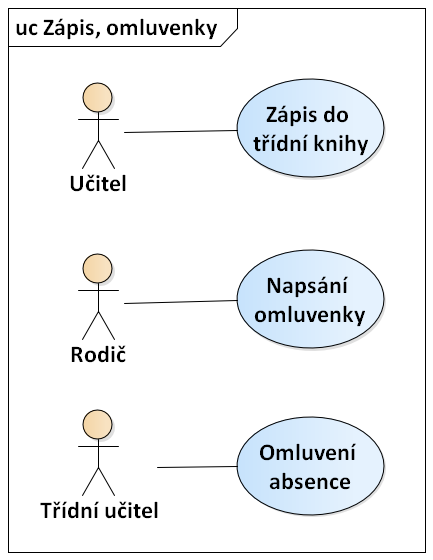
\includegraphics[width=0.5\textwidth]{images/zapis.png}
	\caption{Případy užití pro zápis a omluvenky}
	\label{pripady-zapis}
\end{figure}

\subsubsection*{UC7 Zápis do třídní knihy}
Umožňuje učiteli zapsat záznam o proběhnuté hodině do třídní knihy.
\begin{itemize}
    \item Učitel se přihlásí do systému.
    \item V navigačním menu si vybere políčko, které mu ukáže seznam třídních knih.
    \item Vybere si třídní knihu, do které chce zapsat.
    \item Tím se dostává na stránku, která zobrazuje záznamy v daném dni. Mezi dny lze přepínat.
    \item Stránka obsahuje tlačítko pro vytvoření nového záznamu. Po jeho stisknutí se dostává na formulář, kde může vytvořit nový zápis do třídní knihy.
    \item Ve formuláři vyplní předmět,  téma hodiny, případně číslo hodiny. Po potvrzení je vytvořen nový záznam v třídní knize. 
    \item Pro zadání absence žáků se použije tlačítko v řádku záznamu. 
    \item Po jeho stisknutí se učitel dostane na formulář, kde ze seznamu zaškrtne žáky, kteří nejsou přítomni, případně přišli pozdě.
    \item Potvrzením formuláře se aktualizují absence žáků.
\end{itemize}

\subsubsection*{UC8 Napsání omluvenky}
Umožňuje uživateli s rolí rodič napsat omluvenku, kterou omluví absenci svého potomka.
\begin{itemize}
    \item Rodič se přihlásí do systému.
    \item Přepne se do docházky a vybere potomka, kterého chce zobrazit.
    \item Zobrazí se seznam neomluvených absencí, ze kterých rodič vybere ty, které chce omluvit.
    \item Klikne na tlačítko pro napsání omluvenky.
    \item Dostane se na formulář, kde vyplní text omluvenky.
    \item Potvrzením formuláře omluvenku pošle třídnímu učiteli.
\end{itemize}

\subsubsection*{UC9 Omluvení absence}
Umožňuje třídnímu učiteli omluvit absenci žáka.
\paragraph{Hlavní scénář}
\begin{itemize}
    \item Třídní učitel se přihlásí do systému.
    \item V navigačním menu si vybere políčko pro zobrazení docházky.
    \item Na stránce vidí seznam omluvenek, které čekají na schválení.
    \item Třídní učitel může omluvenku potvrdit či zamítnout, případně si rozkliknout detail, který zobrazí, na které absence se omluvenka vztahuje.
\end{itemize}

\paragraph{Alternativní scénář}
\begin{itemize}
    \item Třídní učitel se přihlásí do systému.
    \item V navigačním menu si vybere políčko pro zobrazení docházky.
    \item Na stránce klikne na tlačítko pro zobrazení absencí žáků.
    \item Zde vidí seznam žáků, kteří mají neomluvené absence.
    \item Vybere žáka, u kterého chce omluvit absenci a klikne na tlačítko pro zobrazení detailu.
    \item Ze seznamu vybere, které absence chce omluvit.
    \item Klikne na tlačítko pro napsání omluvenky.
    \item Dostane se na formulář, kde vyplní text omluvenky a potvrdí.
\end{itemize}

\subsubsection{Události}
Na obrázku \ref{pripady-udalosti} lze vidět případy užití věnující se událostem v hodině.

\begin{figure}[h]
	\centering
	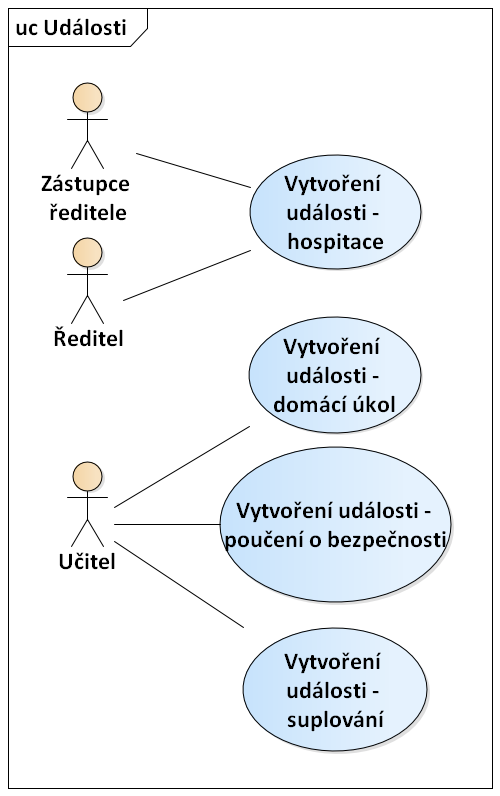
\includegraphics[width=0.6\textwidth]{images/udalosti.png}
	\caption{Případy užití pro události v hodině}
	\label{pripady-udalosti}
\end{figure}

\subsubsection*{UC10 Vytvoření události -- hospitace}
Umožňuje uživateli s rolí ředitel nebo zástupce ředitele přidat do třídní knihy informaci o proběhnuté hospitaci v hodině.

\begin{itemize}
    \item Uživatel s požadovanou rolí se přihlásí do systému.
    \item V navigačním menu se přepne do třídní knihy a vybere třídní knihu třídy, kde bude probíhat hospitace.
    \item Tím se dostává na stránku, která zobrazuje záznamy v daném dni.
    \item U požadované hodiny klikne na tlačítko pro zobrazení menu dalších akcí. 
    \item Ze seznamu vybere tlačítko pro přidání hospitace.
    \item Zobrazí se formulář, kde vyplní jméno hospitujícího a zápis z hospitace. Potvrzením formuláře je hospitace vytvořena.
\end{itemize}


\subsubsection*{UC11 Vytvoření události -- domácí úkol}
Umožňuje učiteli zadat domácí úkol.
\begin{itemize}
    \item Učitel se přihlásí do systému.
    \item V navigačním menu se přepne do třídní knihy a vybere třídní knihu třídy, kde bude zadávat domácí úkol.
    \item Tím se dostává na stránku, která zobrazuje záznamy v daném dni.
    \item U požadované hodiny klikne na tlačítko pro zobrazení menu dalších akcí. 
    \item Ze seznamu vybere tlačítko pro přidání domácího úkolu.
    \item Zobrazí se formulář, kde vyplní název, datum, do kdy má být úkol hotový a zadání úkolu. Potvrzením formuláře úkol vytvoří.
\end{itemize}


\subsubsection*{UC12 Vytvoření události -- suplování}
Umožňuje učiteli zadat informaci o tom, že vyučovací hodina probíhá formou suplování.

\begin{itemize}
    \item Učitel se přihlásí do systému.
    \item V navigačním menu se přepne do třídní knihy a vybere třídní knihu třídy, kde bude probíhat suplování.
    \item Tím se dostává na stránku, která zobrazuje záznamy v daném dni.
    \item U požadované hodiny klikne na tlačítko pro zobrazení menu dalších akcí.
    \item Ze seznamu klikne na tlačítko pro označení suplované hodiny.
\end{itemize}
\subsubsection*{UC13 Vytvoření události -- poučení o bezpečnosti}
Umožňuje uživateli s požadovanou rolí přidat do třídní knihy informaci o tom, že bylo provedeno poučení o bezpečnosti.

\begin{itemize}
    \item Uživatel s požadovanou rolí se přihlásí do systému.

    \item V navigačním menu se přepne do třídní knihy a vybere třídní knihu třídy, kde proběhne poučení o bezpečnosti.
    \item Tím se dostává na stránku, která zobrazuje záznamy v daném dni.
    \item U požadované hodiny klikne na tlačítko pro zobrazení menu dalších akcí. 
    \item Ze seznamu vybere tlačítko pro přidání poučení.
    \item Zobrazí se formulář, kde vyplní název a popis poučení. Potvrzením formuláře se poučení vytvoří.
\end{itemize}


\subsubsection{Administrace}
Na obrázku \ref{pripady-administrace} jsou zobrazeny případy užití, které se věnují administraci uživatelů, předmětů a tříd.

\begin{figure}[h]
	\centering
	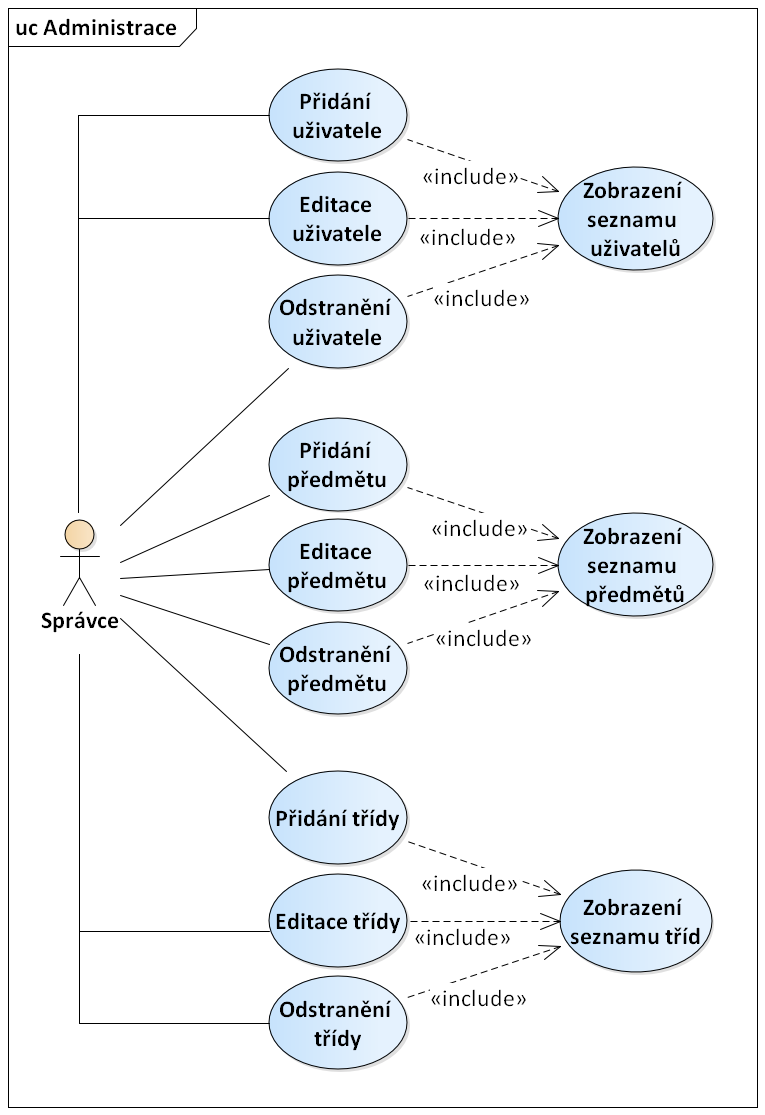
\includegraphics[width=0.80\textwidth]{images/administrace.png}
	\caption{Případy užití pro administraci systému}
	\label{pripady-administrace}
\end{figure}

\subsubsection*{UC14 Přidání uživatele}
Umožňuje správci přidat uživatele do systému. 
\begin{itemize}
    \item Správce se přepne do pohledu se seznamem uživatelů.
    \item Klikne na tlačítko pro přidání uživatele.
    \item Vyplní potřebné informace a potvrdí.
\end{itemize}

\subsubsection*{UC15 Editace uživatele}
Umožňuje správci editovat informace o uživateli.
\begin{itemize}
    \item Správce se přepne do pohledu se seznamem uživatelů.
    \item Klikne na tlačítko pro editaci uživatele.
    \item Změní potřebné informace a potvrdí.
\end{itemize}

\subsubsection*{UC16 Odebrání uživatele}
Umožňuje správci odebrat uživatele ze systému. 
\begin{itemize}
    \item Správce se přepne do pohledu se seznamem uživatelů.
    \item Klikne na tlačítko pro odebrání uživatele.
\end{itemize}

\subsubsection*{UC17 Přidání třídy}
Umožňuje správci přidat třídu do systému. 
\begin{itemize}
    \item Správce se přepne do pohledu se seznamem tříd.
    \item Klikne na tlačítko pro přidání třídy.
    \item Vyplní potřebné informace a potvrdí.
\end{itemize}

\subsubsection*{UC18 Editace třídy}
Umožňuje správci editovat informace o třídě.
\begin{itemize}
    \item Správce se přepne do pohledu se seznamem tříd.
    \item Klikne na tlačítko pro editaci třídy.
    \item Změní potřebné informace a potvrdí.
\end{itemize}

\subsubsection*{UC19 Odebrání třídy}
Umožňuje správci odebrat třídu ze systému. 
\begin{itemize}
    \item Správce se přepne do pohledu se seznamem tříd.
    \item Klikne na tlačítko pro odebrání třídy.
\end{itemize}

\subsubsection*{UC20 Přidání předmětu}
Umožňuje správci přidat předmět do systému. 
\begin{itemize}
    \item Správce se přepne do pohledu se seznamem předmětů.
    \item Klikne na tlačítko pro přidání předmětu.
    \item Vyplní potřebné informace a potvrdí.
\end{itemize}

\subsubsection*{UC21 Editace předmětu}
Umožňuje správci editovat informace o předmětu.
\begin{itemize}
    \item Správce se přepne do pohledu se seznamem předmětů.
    \item Klikne na tlačítko pro editaci předmětu.
    \item Změní potřebné informace a potvrdí.
\end{itemize}

\subsubsection*{UC22 Odebrání předmětu}
Umožňuje správci odebrat předmět ze systému. 
\begin{itemize}
    \item Správce se přepne do pohledu se seznamem předmětů.
    \item Klikne na tlačítko pro odebrání předmětu.
\end{itemize}

\subsubsection*{UC23 Zobrazení seznamu uživatelů}
Umožňuje správci zobrazit seznam uživatelů v systému. Systém umožňuje zobrazení tří skupin uživatelů:
\begin{itemize}
    \item žáků,
    \item rodičů, 
    \item zaměstnanců.
\end{itemize}

\subsubsection*{UC24 Zobrazení seznamu tříd}
Umožňuje správci zobrazit seznam tříd v systému.

\subsubsection*{UC25 Zobrazení seznamu předmětů}
Umožňuje správci zobrazit seznam předmětů v systému.

\section{Architektura}
Architektura informačního systému definuje strukturu systému. Ta se skládá z jednotlivých komponent, jejich vlastností a vztahů mezi nimi \cite{sw-architektura}. Pro tento informační systém bude zvolena třívrstvá architektura, která je vhodná pro složitější aplikace. Třívrstvá architektura rozděluje strukturu systému na tři vrstvy - prezentační, aplikační a datovou.

Prezentační vrstva slouží pro komunikaci s uživatelem. V této vrstvě budou uloženy CSHTML soubory, třídy zpracovávající požadavky od uživatelů, apod. Aplikační vrstva obsahuje business logiku systému. Zde budou probíhat jednotlivé procesy a výpočty. Datová vrstva zajišťuje persistenci dat, nejčastěji s pomocí databáze. V této vrstvě bude probíhat komunikace s databází a budou zde uloženy jednotlivé modely, které představují tabulky v databázi.

\subsection{Moduly}
Informační systém bude rozdělen na moduly podle funkčnosti. Rozdělení na moduly bude probíhat v každé vrstvě třívrstvé architektury a zajistí splnění nefunkčního požadavku N3, který požaduje snadnou rozšiřitelnost systému.

Na obrázku \ref{architektura} je zobrazen návrh architektury systému. Datová vrstva bude používat Entity Framework Core, který slouží k mapování objektů na relační data. Využíván bude v kombinaci s návrhovým vzorem repository. Každý modul bude mít své vlastní repository, které bude obsahovat dotazy do databáze.

V aplikační vrstvě budou všechny moduly rozděleny do vlastních funkčních celků, ve kterých budou probíhat procesy a funkcionalita spojená s daným modulem. 

Co se prezentační vrstvy týče, každý modul bude používat návrhový vzor MVC (model-view-controller), který řeší problémy prezentační vrstvy. Návrhový vzor MVC rozděluje strukturu kódu na tři vrstvy -- modely, views (pohledy) a controllers (kontrolery).

Model je nejnižší vrstva tohoto vzoru. Je tvořen doménovými objekty a reprezentuje data aplikace. Pomocí těchto objektů se předávají data do pohledů a z pohledů do kontrolerů. Pohledy se starají o uživatelské rozhraní. Tato vrstva se skládá z HTML šablon,  do kterých lze vkládat data z kontrolerů. V šablonách lze kombinovat čisté HTML s server-side kódem. Kontrolery se starají o zpracovávání uživatelských požadavků z pohledů. Každý požadavek je pomocí routování mapován na určitou akci v kontroleru. Zjednodušeně lze říci, že kontrolery řídí celkový průchod aplikací. \cite{dp-mvc} 
\clearpage

\begin{figure}[h]
	\centering
	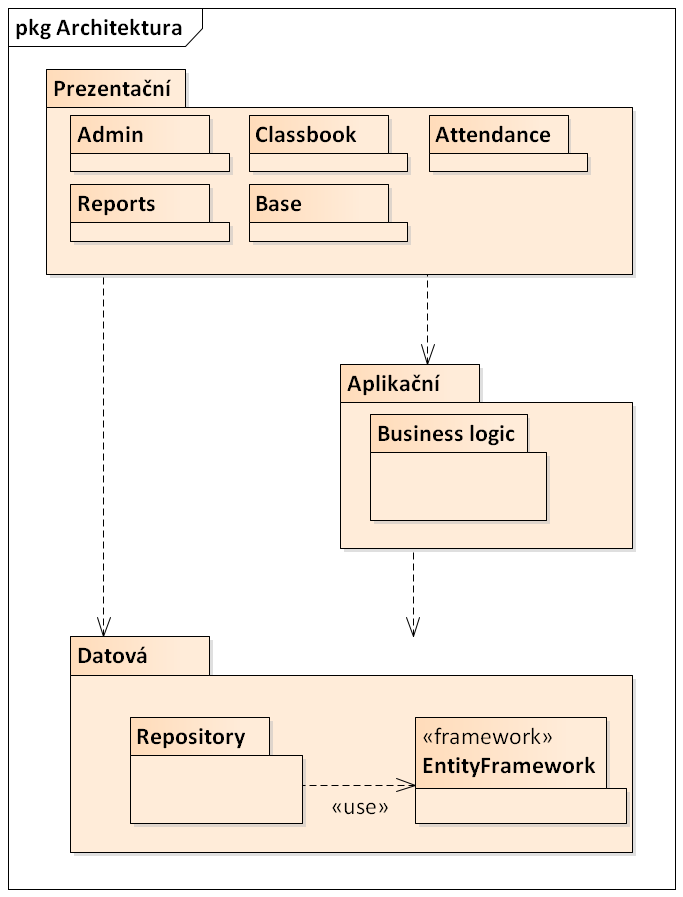
\includegraphics[width=0.8\textwidth]{images/architektura.png}
	\caption{Třívrstvá architektura - relaxovaná}
	\label{architektura}
\end{figure}

Informační systém je rozdělen na následujících pět modulů.

\subsubsection*{Modul administrace - Admin}
Modul administrace slouží pro správu systému. Tento modul zajistí splnění funkčního požadavku F2. Do této sekce bude mít přístup pouze uživatel s rolí správce. Bude zde probíhat správa uživatelů, tříd a předmětů.

\subsubsection*{Modul třídní knihy - Classbook}
V tomto modulu bude probíhat práce s třídní knihou. Tento modul bude pokrývat funkční požadavky F3, F5 a F7. Do této sekce budou mít přístup všichni uživatelé s rolí učitel, třídní učitel, zástupce ředitele, ředitel a správce. Budou zde probíhat zápisy do třídních knih, vytváření událostí v hodinách a exporty třídních knih.

\subsubsection*{Modul docházka - Attendance}
Zde bude probíhat veškerá práce s omluvenkami. Modul docházka zajistí pokrytí funkčního požadavku F4. Modul bude dostupný uživatelům s rolí rodič a třídní učitel. Rodič zde bude vytvářet omluvenky a odesílat je třídnímu učiteli. Třídní učitel bude v tomto modulu omlouvat absenci žáka na základě omluvenek od rodiče.

\subsubsection*{Modul přehledy - Reports}
Pomocí tohoto modulu budou zobrazovány přehledy o žácích, čímž se splní funkční požadavek F6. Zde budou mít přístup všichni přihlášení uživatelé. Uživatelům z řad zaměstnanců budou poskytnuty přehledy o všech žácích. Rodičům, respektive žákům budou zobrazeny přehledy pouze o potomcích, respektive o sobě.

\subsubsection*{Základní modul - Base}
V základním modulu budou probíhat obecné funkcionality, například autentizace a autorizace. Tento modul splní funkční požadavek F1. Jelikož se v tomto modulu budou vyskytovat pouze obecné funkcionality, bude přístupný všem uživatelům.


\section{Návrh obrazovek}
V této části bude navrhnuto uživatelské rozhraní několika hlavních obrazovek. Vždy bude navržena pouze základní kostra obrazovky, finální design aplikace bude vyřešen až při její implementaci.

Základní kostra bude navržena pro obrazovku, kde probíhá zápis do třídní knihy, pro obrazovku, kde třídní učitel schvaluje omluvenky a pro úvodní stránku rodičovského portálu.
\clearpage

Na obrázku \ref{obrazovka-zapis} je zobrazena obrazovka pro zápis do třídní knihy. Lze vidět, že zápis se vztahuje k vybranému datu. To lze vybrat po rozkliknutí kalendáře. Defaultně se vyplňuje aktuální datum. Zápis se vytváří pomocí tlačítka pro nový zápis, které přesměruje uživatele na formulář, kde se vyplní předmět a téma. Absence se vyplní ve formuláři, který se vyvolá stisknutím tlačítka \uv{Absence}. Případné události se vyberou ze seznamu po stisknutí tlačítka \uv{Další}.

\begin{figure}[h]
	\centering
	\frame{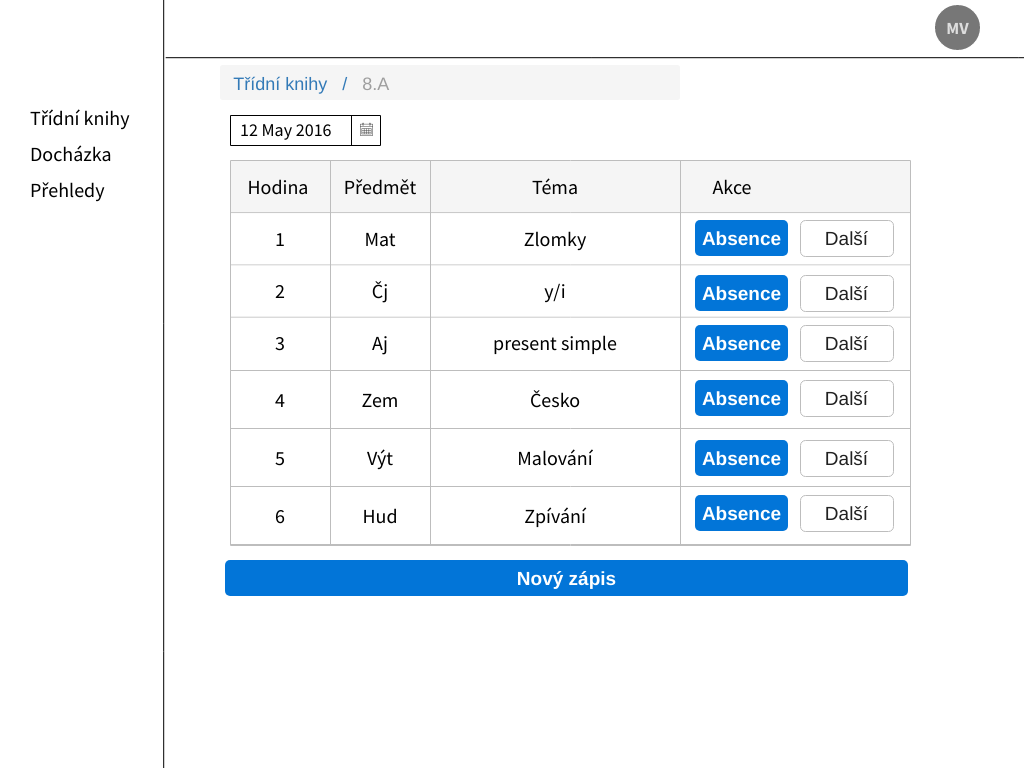
\includegraphics[width=\textwidth]{images/obrazovka_zapis.png}}
	\caption{Obrazovka pro zápis do třídní knihy}
	\label{obrazovka-zapis}
\end{figure}

Na obrázku \ref{obrazovka-omluvenky} lze vidět obrazovku, kde třídní učitel schvaluje omluvenky. Třídní učitel vidí seznam omluvenek, které může potvrdit či zamítnout. Může si také zobrazit detail, kde uvidí, pro které absence je omluvenka napsána.
\clearpage

\begin{figure}[h]
	\centering
	\frame{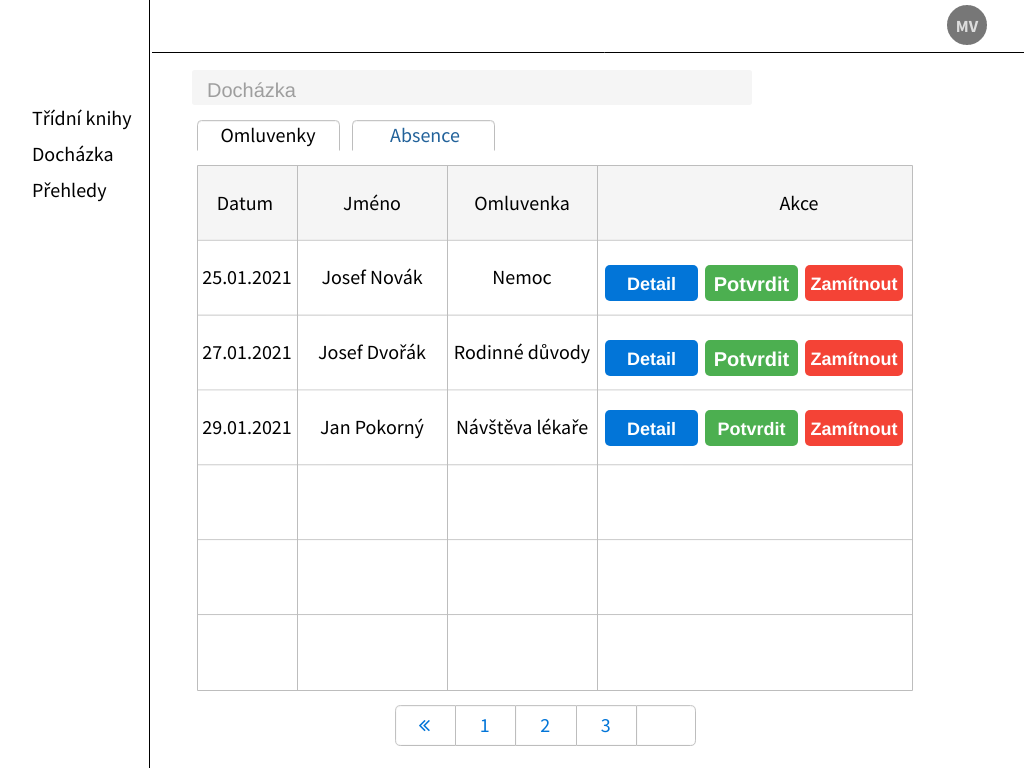
\includegraphics[width=\textwidth]{images/obrazovka_omluvenky.png}}
	\caption{Obrazovka pro schvalování omluvenek}
	\label{obrazovka-omluvenky}
\end{figure}

Obrázek \ref{obrazovka-rodic} zobrazuje návrh rodičovského portálu. Rodič vidí seznam svých dětí a rychlý přehled o nových informacích. Detaily o těchto informacích si rodič může zjistit v příslušných přehledech. Do nich se přepne pomocí navigačního menu vlevo stránky.
\clearpage

\begin{figure}[H]
	\centering
	\frame{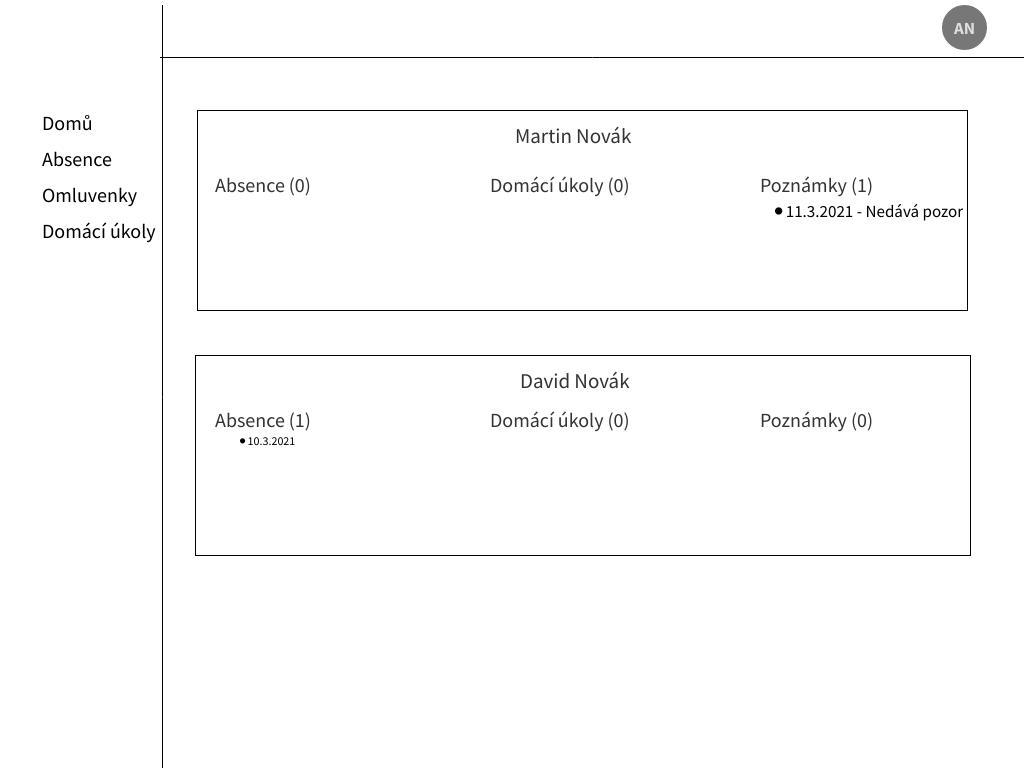
\includegraphics[width=\textwidth]{images/obrazovka_rodic.png}}
	\caption{Prostředí pro rodiče}
	\label{obrazovka-rodic}
\end{figure}




\chapter{Realizace}
Tato kapitola je věnována realizaci navrhovaného systému. Kapitola je rozdělena na dvě podkapitoly a to na implementaci a testování.

V části zaměřené na implementaci jsou popsány použité technologie, je představena struktura jednotlivých modulů a jsou zde popsány jednotlivá rozhraní, třídy a pohledy. Další částí v této podkapitole jsou implementační poznámky, kde jsou popsány použité knihovny a řešení autentizace a autorizace.

V druhé části zaměřené na testování je popsán průběh testování systému a výsledky testování.

\section{Implementace}

\subsection{Použité technologie}
Vyvíjený informační systém lze rozdělit na tři dílčí části. První částí je backend aplikace. To je část, která se stará o logiku aplikace, plnění funkcí systému a zpracovávání procesů. Druhou částí je frontend, ten se stará o vzhled aplikace. Je to část systému, se kterou pracuje koncový uživatel. Poslední částí je databáze, kam se ukládají potřebná data.

\subsubsection{Backend}
Backend systému je vyvíjen na platformě .NET Core s použitím jazyka C\# a ASP.NET Core MVC frameworku. Volba platformy .NET Core je dána ze zadání práce.

.NET Core je open-source platforma vyvíjená a podporovaná společností Microsoft. V rámci této platformy lze vyvíjet webové, desktopové, konzolové či mobilní aplikace, programy pro IoT a další. Aplikace lze vyvíjet pro velkou škálu operačních systémů, nejen pro Microsoft Windows. Lze vytvářet programy i pro operační systém Linux, macOS, Android, iOS a další. Aplikace mohou být i multiplatformní, což znamená, že jedna aplikace může být spuštěna na vícero různých operačních systémech. \cite{net-introduction} 

ASP.NET Core MVC je open-source framework pro tvorbu webových aplikací na platformě .NET Core. Tento framework poskytuje programátorovi zázemí pro vytváření aplikací s MVC architekturou. Obsahuje mimo jiné i systém pro routování, který umožňuje programátorovi definovat, jakým způsobem se budou zpracovávat URL adresy, systém pro binding modelů, který umožňuje předávat objekty do HTML šablon, a vestavěnou podporu pro dependency injection \cite{net-mvc-overview}, což je návrhový vzor k dosažení IoC (Inversion of Control) mezi třídami a jejich závislostmi \cite{net-dependency-injection}. V ASP.NET Core MVC se závislosti předávají do třídy pomocí konstruktoru, jehož parametry tvoří vkládané závislosti (rozhraní). Konkrétní implementace, které budou nakonec použity a jakým způsobem se vytvoří, se určí ve třídě \texttt{Startup.cs}. Programy v tomto frameworku mohou být vyvíjeny a provozovány v operačních systémech Microsoft Windows, Linux i macOS \cite{net-core-introduction}.

Zdrojový kód je napsán v jazyce C\#, což je objektově orientovaný a typově bezpečný programovací jazyk od společnosti Microsoft.

Backend aplikace se na rozdíl od frontend části vyznačuje tím, že je provozován na serveru, na který poté přichází požadavky od klienta. Požadavek může chtít vrátit celou webovou stránku, určitá data a jiné. Ve vyvíjeném systému požadavek typicky žádá o webovou stránku. Celý proces začíná tím, že klient pošle požadavek na server s cílem získat určitou webovou stránku. Server zavolá ASP.NET Core, který podle URL adresy pozná, co klient požaduje. V případě potřeby si program zajistí data a poté, pomocí vytvořených šablon, sestaví webovou stránku, kterou pošle klientovi zpět.

\subsubsection{Frontend}
Frontend je primárně vytvořen pomocí HTML šablon, které se používají při vývoji ASP.NET Core MVC aplikací, a doplněn jazykem CSS, Bootstrap frameworkem a JavaScriptem. 
V návrhovém vzoru MVC (model-view-controller) se HTML šablony nachází ve view vrstvě (vrstvě pohledů). Každá šablona představuje webovou stránku nebo její část. Tato šablona může obsahovat HTML nebo C\# kód, ten je do šablon vkládán pomocí značkovacího jazyka Razor. Tyto šablony lze poznat podle toho, že mají příponu \texttt{.cshtml}. \cite{net-views}

CSS (Cascading Style Sheets) je jazyk, pomocí kterého se definují styly HTML elementů. Popisuje se s ním například layout stránky, barva a velikost elementu, apod. Lze s nimi také popisovat HTML elementy na základě velikosti obrazovky zařízení. \cite{css}

Bootstrap je bezplatný, open-source framework, který usnadňuje vývoj frontend části webových stránek. Obsahuje velké množství předpřipravených HTML a CSS komponent, například tlačítka, tabulky, navigační panely a další. Framework také umožňuje programátorovi jednoduše řešit problém responzivity webových stránek (zobrazení na zařízeních s různou velikostí displeje). V tomto projektu Bootstrap pomohl jak se vzhledem stránky, tak při řešení responzivity. Oproti konkurenčním projektům nabízí především větší uživatelskou základnu, jedná se totiž o nejpopulárnější framework svého druhu. \cite{bootstrap-w3s, bootstrap}

Posledním použitým nástrojem je JavaScript resp. jQuery \cite{jquery}. JavaScript je skriptovací jazyk, který umožňuje vytvářet dynamický obsah na webových stránkách, a to u klienta ve webovém prohlížeči \cite{what-is-js}. Lze ho použít například pro uložení nějaké informace do proměnné či reagovat na nějakou akci, kterou uživatel provede \cite{what-is-js}. jQuery je knihovna napsaná v JavaScriptu, která usnadňuje práci se zpracováním událostí, manipulací obsahu HTML stránky a další. Tyto technologie využívá v projektu především Bootstrap framework, využity byly také při zobrazování postranního navigačního panelu u zařízení s menším displejem. Hlavním důvodem použití jQuery oproti alternativám (např. React \cite{react}) byl fakt, že tuto knihovnu již využívá Bootstrap framework. Navíc knihovna byla použita pro řešení velmi jednoduchých problémů typických právě pro jQuery.

Frontend aplikace je provozován na straně klienta, odkud jsou poté přechodem na jinou URL adresu posílány požadavky na server.

\subsubsection{Databáze}
Pro uchovávání dat, se kterými aplikace pracují se využívají databáze. Ty se dělí na několik druhů, například relační, nerelační (NoSQL), grafové, distribuované a další. Výběr typu databáze záleží na tom, jakým způsobem budou data používána. Například NoSQL se používá pro ukládání nestrukturovaných dat nebo dat, nad kterými se budou provádět složité vyhledávací operace. Pro aplikaci vyvíjenou v rámci této práce byla z důvodu nutnosti integrity dat a faktu, že data mají mezi sebou jasně definované vztahy, zvolena relační databáze, která je pro tyto omezení vhodná. \cite{co-je-sql, sql-vs-nosql}

Pro vývoj databáze byl použit Entity Framework Core s code-first přístupem. Entity Framework Core je ORM framework, který umožňuje vývojáři pracovat s tabulkami databáze jako s objekty. Umožňuje mapovat třídy jako tabulky databáze, provádět SQL příkazy pomocí LINQ (Language Integrated Query) či ukládat data do databáze. Pro přístup k datům je nejprve nutné definovat tzv. model, ten je tvořen entitními třídami a databázovým kontextem. Model mapuje entity a vztahy na tabulky v databázi. Databázový kontext je objekt, který udržuje relaci s databází a probíhají pomocí něj dotazy do databáze či ukládání dat \cite{ef-core}. V aplikaci to vypadá tak, že pro tabulku je vytvořena třída, která obsahuje vlastnosti (property), které odpovídají sloupcům v tabulce. V třídě databázového kontextu poté lze třídám/tabulkám přiřazovat různé vztahy a vlastnosti, například cizí klíče, informaci, jestli může být sloupec prázdný, apod. Databázový kontext dále obsahuje informace o použité databázi a kolekce entitních tříd, které obsahují všechny dostupné entity (záznamy) daného typu.

Code-first přístup je technika, která umožňuje vytvořit a udržovat databázi a její tabulky pomocí zdrojového kódu na platformě .NET Core \cite{code-first}. Znamená to tedy, že databáze ani tabulky se nevytváří a neupravují pomocí SQL skriptů ručně, ale všechny vlastnosti a vztahy mezi tabulkami se definují v entitních třídách a databázovém kontextu. Vytváření a přenos změn v databázi poté zajišťuje Entity Framework Core pomocí tzv. migrací, které převedou definovaný zdrojový kód do databáze/tabulek. Entity Framework Core nabízí kromě code-first ještě jeden další přístup. Tím je databázový přístup. Ten spočívá v tom, že databáze již existuje nebo je vytvořena samostatně. Entity Framework Core poté vytvoří model (entitní třídy a databázový kontext) podle tabulek v databázi \cite{ef-core}. Výhodou code-first přístupu je, že není potřeba využívat další nástroj pro tvorbu schématu databáze, všechny změny, které se pomocí migrace dostanou do databáze, jsou sledovány a mohou být snadno vráceny zpět. Vývojář má také kontrolu nad tím, jak databáze vypadá a funguje, protože se vyhne automaticky generovanému kódu. Z těchto důvodů byl pro vyvíjený systém zvolen code-first přístup.

Entity Framework Core umí pracovat s celou řadou databází pomocí stažitelných knihoven. Dokáže pracovat například s Microsoft SQL Server 2012 a novější, SQLite 3.7 a novější, PostgreSQL, MySQL, Oracle DB a další \cite{database-providers}. Při vývoji byla použita databáze Microsoft SQL Server. Aplikace je připravena na provoz jak s Microsoft SQL Server, tak s PostgreSQL databází. Podpora obou těchto databází poskytuje větší možnosti školám při provozu aplikace. Postup, jak aplikaci nasadit, je popsán v instalační příručce, která je součástí přílohy této práce.

\subsection{Prezentační vrstva}
Prezentační vrstva je rozdělena do tzv. oblastí (areas), ty umožňují rozdělit zdrojový kód v ASP.NET Core MVC aplikaci do menších funkčních celků \cite{areas}. Každý modul, kromě základního modulu Base, má vlastní oblast. Zdrojový kód Base modulu je umístěn v root adresáři projektu. Každý modul je podle návrhu rozdělen na modely, pohledy a kontrolery. Strukturu projektu pro prezentační vrstvu můžeme vidět na obrázku \ref{struktura-projektu}.
\clearpage

\begin{figure}[h]
	\centering
	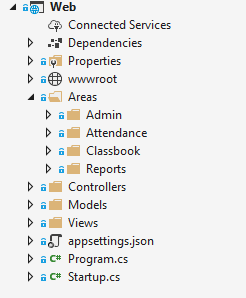
\includegraphics[width=0.5\textwidth]{images/struktura_projektu.png}
	\caption{Struktura projektu prezentační vrstvy}
	\label{struktura-projektu}
\end{figure}

\subsubsection{Základní modul -- Base}
Základní modul je umístěn v root adresáři projektu Web. Modul obsahuje tyto kontrolery:
\begin{itemize}
    \item \texttt{AccountController}
    \begin{itemize}
        \item Kontroler slouží pro obecnou práci s uživateli. Umožňuje uživateli přihlášení do systému, odhlášení, změnu hesla a zobrazení základních informací o účtu. Práce s tímto kontrolerem není omezena na žádnou roli uživatele, některé metody však požadují přihlášeného uživatele.
    \end{itemize}
    \item \texttt{HomeController}
    \begin{itemize}
        \item Úlohou tohoto kontroleru je přesměrování přihlášeného uživatele na jeho domovskou stránku. Například rodiče přesměruje na stránku s rychlým přehledem o jeho dětech, admina přesměruje na stránku, kde se provádí administrace. Tento kontroler požaduje přihlášeného uživatele.
    \end{itemize}
\end{itemize}

\clearpage
Přehled pohledů podle kontrolerů:

\begin{itemize}
    \item \texttt{AccountController}
    \begin{itemize}
        \item \texttt{AccessDenied} -- V případě odepření přístupu systém přesměruje uživatele na tuto stránku.
        \item \texttt{ForgotPassword} -- Stránka, kde nepřihlášený uživatel požádá o obnovu zapomenutého hesla.
        \item \texttt{ChangePassword} -- Stránka obsahující formulář pro změnu hesla.
        \item \texttt{Login} -- Stránka pro přihlášení uživatele.
        \item \texttt{ResetPassword} -- Stránka, kde nepřihlášený uživatel zadá své nové heslo.
        \item \texttt{UserAccount} -- Stránka se základními informacemi o účtu.
    \end{itemize}
\end{itemize}

Tento modul obsahuje i pohled, který je sdílený téměř v celé aplikaci. Jedná se o layout s hlavičkou a postranním navigačním panelem.


\subsubsection{Modul administrace -- Admin}
Modul pro administraci je umístěn v oblasti Admin. Modul obsahuje následující kontrolery:
\begin{itemize}
    \item \texttt{ClassController}
    \begin{itemize}
        \item Kontroler slouží pro správu tříd ve škole. Umožňuje uživateli s rolí správce přidávat nové třídy, upravovat údaje o třídách či mazat stávající třídy.
    \end{itemize}
    
    \item \texttt{SubjectController}
    \begin{itemize}
        \item Kontroler slouží pro správu vyučovaných předmětů. Umožňuje uživateli s rolí správce přidávat nové předměty, upravovat údaje o předmětech či mazat stávající předměty.
    \end{itemize}
    \item \texttt{UserController}
    \begin{itemize}
        \item Kontroler umožňuje uživateli s rolí správce přidávat, upravovat či mazat uživatele v systému.
    \end{itemize}
\end{itemize}

Přehled pohledů podle kontrolerů:
\begin{itemize}
    \item \texttt{ClassController}
    \begin{itemize}
        \item \texttt{AddClass} -- Stránka s formulářem pro přidání třídy.
        \item \texttt{DetailClass} -- Stránka, která zobrazí detailní informace o třídě.
        \item \texttt{EditClass} -- Stránka umožňující úpravu údajů o třídě.
        \item \texttt{Index} -- Stránka, která zobrazí seznam tříd.
    \end{itemize}
    
    \item \texttt{SubjectController}
    \begin{itemize}
        \item \texttt{AddSubject} -- Stránka s formulářem pro přidání předmětu.
        \item \texttt{DetailSubject} -- Stránka, která zobrazí detailní informace o předmětu.
        \item \texttt{EditSubject} -- Stránka umožňující úpravu údajů o předmětu.
        \item \texttt{Index} -- Stránka, která zobrazí seznam předmětů.
    \end{itemize}
    
    \item \texttt{UserController}
    \begin{itemize}
        \item \texttt{AddEmployee} -- Stránka s formulářem pro přidání zaměstnance.
        \item \texttt{AddParent} -- Stránka s formulářem pro přidání rodiče.
        \item \texttt{AddStudent} -- Stránka s formulářem pro přidání žáka.
        \item \texttt{DetailEmployee} -- Stránka, která zobrazí detailní informace o zaměstnanci.
        \item \texttt{DetailParent} -- Stránka, která zobrazí detailní informace o rodiči.
        \item \texttt{DetailStudent} -- Stránka, která zobrazí detailní informace o žákovi.
        \item \texttt{EditEmployee} -- Stránka umožňující úpravu údajů o zaměstnanci.
        \item \texttt{EditParent} -- Stránka umožňující úpravu údajů o rodiči.
        \item \texttt{EditStudent} -- Stránka umožňující úpravu údajů o žákovi.
        \item \texttt{EmployeeList} -- Stránka, která zobrazí seznam zaměstnanců.
        \item \texttt{ParentList} -- Stránka, která zobrazí seznam rodičů.
        \item \texttt{StudentList} -- Stránka, která zobrazí seznam žáků.
    \end{itemize}
\end{itemize}

Modul obsahuje ještě jeden pohled, který je použit všemi ostatními pohledy. Jedná se o layout, který obsahuje navigační prvky.

\subsubsection{Modul třídní knihy -- Classbook}
Modul pro práci s třídní knihou je umístěn v oblasti Classbook. Modul obsahuje následující kontrolery:
\begin{itemize}
    \item \texttt{ClassbookController}
    \begin{itemize}
        \item Kontroler slouží pro práci s určitou třídní knihou. Umožňuje přidávat a upravovat záznamy o proběhnuté hodině, vyplňovat docházku a přidávat události. S kontrolerem mohou pracovat pouze uživatelé s rolí správce, ředitel, zástupce ředitele, třídní učitel a učitel. Některé metody v kontroleru jsou však omezeny ještě více, například přidat záznam o proběhnuté hodině může pouze učitel.
    \end{itemize}
    
    \item \texttt{HomeController}
    \begin{itemize}
        \item Kontroler slouží především pro správu třídních knih. Umožňuje přidávat nové třídní knihy a upravovat či mazat stávající. Dále umožňuje exportovat třídní knihu do PDF souboru.
    \end{itemize}
    
    \item \texttt{InspectionController}
    \begin{itemize}
        \item Kontroler slouží pro přehled a správu vytvořených hospitací. Umožňuje správci, řediteli, zástupci ředitele, třídnímu učiteli a učiteli zobrazit detail hospitace a řediteli a zástupci ředitele umožňuje smazat vybranou hospitaci.
    \end{itemize}
    
    \item \texttt{InstructionController}
    \begin{itemize}
        \item Kontroler slouží pro přehled a správu vytvořených poučení. Umožňuje uživatelům s rolí správce, ředitel, zástupce ředitele, třídní učitel a učitel zobrazit detail nebo smazat vybrané poučení.
    \end{itemize}
    
    \item \texttt{StudentController}
    \begin{itemize}
        \item Tento kontroler slouží pro přehled žáků ve třídě, dále umožňuje vytvořit poznámku o chování žáka, případně zobrazit jejich seznam. Kontroler je přístupný uživatelům s rolí správce, ředitel, zástupce ředitele, třídní učitel a učitel. Vytvářet poznámky může pouze uživatel s rolí učitel.
    \end{itemize}
\end{itemize}

Přehled pohledů podle kontrolerů:

\begin{itemize}
    \item \texttt{ClassbookController}
    \begin{itemize}
         \item \texttt{AddAttendance} -- Stránka s formulářem pro vyplnění docházky žáků v hodině.
         \item \texttt{AddHomework} -- Stránka s formulářem pro vytvoření nového domácího úkolu.
         \item \texttt{AddInspection} -- Stránka s formulářem pro vytvoření hospitace.
         \item \texttt{AddInstruction} -- Stránka s formulářem pro vytvoření poučení.
         \item \texttt{AddRecord} -- Stránka obsahující formulář, který vytvoří záznam v třídní knize o proběhnuté hodině.
         \item \texttt{DetailHomework} -- Stránka, která zobrazí detailní informace o domácím úkolu.
         \item \texttt{EditRecord} -- Stránka pro upravení záznamu o proběhnuté hodině.
         \item \texttt{Index} -- Stránka zobrazující seznam záznamů v daný den.
         \item \texttt{ShowHomeworks} -- Stránka zobrazující seznam se zadanými domácími úkoly.
    \end{itemize}
    
    \item \texttt{HomeController}
    \begin{itemize}
        \item \texttt{AddClassbook} -- Stránka obsahující formulář pro vytvoření nové třídní knihy.
        \item \texttt{EditClassbook} -- Stránka pro úpravu údajů o třídní knize.
        \item \texttt{ExportClassbook} -- Stránka s formulářem pro export třídní knihy.
        \item \texttt{Index} -- Stránka zobrazující seznam třídních knih.
    \end{itemize}
    
    \item \texttt{InspectionController}
    \begin{itemize}
        \item \texttt{DetailInspection} -- Stránka zobrazující detailní informace o ho\-spitaci.
        \item \texttt{Index} -- Stránka zobrazující seznam provedených hospitací.
    \end{itemize}
    
    \item \texttt{InstructionController}
    \begin{itemize}
        \item \texttt{DetailInstruction} -- Stránka, která zobrazí detailní informace o poučení.
        \item \texttt{Index} -- Stránka zobrazující seznam poučení.
    \end{itemize}
    
    \item \texttt{StudentController}
    \begin{itemize}
        \item \texttt{CreateSchoolHomeNote} -- Stránka s formulářem pro vytvoření poznámky o chování žáka.
        \item \texttt{Index} -- Stránka zobrazující seznam žáků.
        \item \texttt{ListSchoolHomeNote} -- Stránka, která zobrazuje seznam poznámek o chování určitého žáka.
    \end{itemize}
\end{itemize}

Modul obsahuje ještě další dva pohledy. Prvním z nich je layout stránky, který obsahuje navigační prvky, ten je použit v ostatních pohledech. Druhým je CSHTML dokument, který tvoří šablonu pro generovaný PDF soubor.

\subsubsection{Modul docházky -- Attendance}
Modul pro práci s omluvenkami je umístěn v oblasti Attendance. Modul obsahuje následující kontrolery:
\begin{itemize}
    \item \texttt{ClassTeacherController}
    \begin{itemize}
        \item Tento kontroler mohou využívat pouze uživatelé s rolí třídní učitel. Slouží pro potvrzování omluvenek, přehled absencí žáků a případné omluvení těchto absencí.
    \end{itemize}
    
    \item
    \texttt{ParentController}
    \begin{itemize}
        \item Tento kontroler je přístupný pouze rodičům a slouží pro omlouvání absence žáka.
    \end{itemize}
\end{itemize}

Přehled pohledů podle kontrolerů:

\begin{itemize}
    \item \texttt{ClassTeacherController}
    \begin{itemize}
        \item \texttt{ShowAbsentNotes} -- Stránka zobrazující seznam omluvenek k potvrzení.
        \item \texttt{ShowStudentAbsences} -- Stránka zobrazí seznam absencí vybraného žáka.
        \item \texttt{ShowStudents} -- Stránka se seznamem žáků, které mají neomluvené absence.
        \item \texttt{ToBeCreatedAbsentNote} -- Stránka s formulářem pro omluvení absence.
    \end{itemize}
    
    \item \texttt{ParentController}
    \begin{itemize}
        \item \texttt{CreateAbsentNote} -- Stránka s formulářem pro vytvoření omluvenky.
        \item \texttt{ShowAbsences} -- Stránka zobrazující seznam neomluvených absencí vybraného žáka.
    \end{itemize}
\end{itemize}

Modul obsahuje dva další pohledy. V obou případech se jedná o layout, který obsahuje navigační prvky. V prvním případě se jedná o layout pro pohledy kontroleru ClassTeacherController, v druhém případě o layout pro pohledy kontroleru ParentController.


\subsubsection{Modul přehledy -- Reports}
Modul pro zobrazování přehledů je umístěn v oblasti Reports. Modul obsahuje následující kontrolery:

\begin{itemize}
    \item \texttt{ParentController}
    \begin{itemize}
        \item Kontroler je přístupný pouze uživateli s rolí rodič a umožňuje zobrazit přehled o jeho dětech.
    \end{itemize}
    
    \item \texttt{ReportController}
    \begin{itemize}
        \item Tento kontroler je přístupný uživatelům s rolí správce, ředitel, zástupce ředitele, třídní učitel a učitel. Umožňuje zobrazit přehled o žácích podle třídy a uživatelům s rolí učitel a třídní učitel zobrazit rychlý přehled.
    \end{itemize}
    
    \item \texttt{StudentController}
    \begin{itemize}
        \item Kontroler je přístupný pouze uživateli s rolí žák a umožňuje mu zobrazit přehled o sobě samém.
    \end{itemize}
\end{itemize}

Přehled pohledů podle kontrolerů:

\begin{itemize}
    \item \texttt{ParentController}
    \begin{itemize}
        \item \texttt{DetailHomework} -- Stránka zobrazující detailní informace o vybraném domácím úkolu.
        \item \texttt{Index} -- Stránka s rychlým přehledem pro rodiče. Zobrazuje neomluvené absence, domácí úkoly a poznámky o chování. Informace jsou rozděleny podle žáka.
        \item \texttt{ShowAbsentNotes} -- Stránka zobrazí seznam odeslaných omluvenek.
        \item \texttt{ShowHomeworks} -- Stránka zobrazující seznam domácích úloh vybraného žáka.
        \item \texttt{ShowSchoolHomeNotes} -- Zobrazí seznam poznámek o chování vybraného žáka.
    \end{itemize}
    
    \item \texttt{ReportController}
    \begin{itemize}
        \item \texttt{DetailHomework} -- Stránka zobrazující detailní informace o vybraném domácím úkolu.
        \item \texttt{Index} -- Stránka zobrazí seznam žáků podle vybrané třídy.
        \item \texttt{ShowAbsences} -- Stránka zobrazující seznam omluvených a neomluvených absencí vybraného žáka.
        \item \texttt{ShowSchoolHomeNotes} -- Stránka, která zobrazuje seznam poznámek o chování vybraného žáka.
        \item \texttt{ShowHomeworks} -- Stránka, která zobrazuje seznam domácích úkolů, které má vybraný žák vypracovat.
        \item \texttt{TeacherDashBoard} -- Stránka zobrazující rychlý přehled pro učitele a třídní učitele. Obsahuje připomínku domácích úloh a zobrazuje omluvenky čekající na potvrzení.
    \end{itemize}
    
    \item \texttt{StudentController}
    \begin{itemize}
        \item \texttt{DetailHomework} -- Stránka zobrazující detailní informace o vybraném domácím úkolu.
        \item \texttt{Index} -- Stránka s rychlým přehledem pro žáka. Zobrazí neomluvené absence, domácí úkoly a poznámky o chování.
        \item \texttt{ShowAbsences} -- Zobrazí seznam omluvených i neomluvených absencí.
        \item \texttt{ShowAbsentNotes} -- Zobrazí seznam odeslaných omluvenek.
        \item \texttt{ShowHomeworks} -- Stránka zobrazující seznam domácích úloh, které má žák splnit.
        \item \texttt{ShowSchoolHomeNotes} -- Zobrazí seznam poznámek o chování.
    \end{itemize}
\end{itemize}

Modul obsahuje několik dalších pohledů. Ve všech případech se jedná o layout s navigačními prvky. 


\subsection{Aplikační vrstva}
Aplikační vrstva je podobně jako prezentační vrstva rozdělena podle modulů. Pro každý modul byl vytvořen samostatný projekt, který obsahuje seznam rozhraní a třídy s implementací. Tato vrstva obsahuje ještě jeden projekt, který slouží pro obecnou funkcionalitu, která logicky nepatří do projektů s moduly. Jedná se o projekt Common, který obsahuje jednu třídu, která pomáhá se stránkováním seznamu prvků v tabulkách.

\subsubsection{Základní modul -- Base}
Základní modul se nachází v projektu Base, který se stará o obecnou funkcionalitu systému. V projektu nalezneme třídy pro práci s e-maily a uživatelem. Projekt Base obsahuje následující rozhraní:
\begin{itemize}
    \item \texttt{IEmailService}
    \begin{itemize}
        \item Jedná se o rozhraní, které poskytuje metodu pro odesílání e-mailu.
    \end{itemize}
    
    \item \texttt{IUserManager}
    \begin{itemize}
        \item Jedná se o rozhraní, které poskytuje metody pro práci s uživatelem, například ověření uživatele vůči databázi pomocí e-mailu a hesla.
    \end{itemize}
\end{itemize}

Projekt Base obsahuje následující třídy:
\begin{itemize}
    \item \texttt{EmailService}
    \begin{itemize}
        \item Jedná se o implementaci rozhraní \texttt{IEmailService}.
    \end{itemize}
    
    \item \texttt{PasswordHasher}
    \begin{itemize}
        \item Třída poskytující metody pro práci s heslem. Dokáže ověřovat a tvořit hash z hesla.
    \end{itemize}
    
    \item \texttt{SecurityHelper}
    \begin{itemize}
        \item Třída poskytuje metodu pro tvorbu bezpečnostního tokenu, který slouží při obnově zapomenutého hesla.
    \end{itemize}
    
    \item \texttt{UserManager}
    \begin{itemize}
        \item Jedná se o implementaci rozhraní \texttt{IUserManager}.
    \end{itemize}
\end{itemize}


\subsubsection{Modul administrace -- Admin}
Modul pro administraci se nachází v projektu Admin. Ten se stará o administraci uživatelů, předmětů a tříd ve škole. V projektu nalezneme jediné rozhraní a jednu implementaci rozhraní. Projekt Admin obsahuje následující rozhraní:
\begin{itemize}
    \item \texttt{IAdminManager}
    \begin{itemize}
        \item Rozhraní poskytuje metody pro správu uživatelů, předmětů a tříd. Tedy především metody pro přidávání, editování nebo mazání. 
    \end{itemize}
\end{itemize}

Projekt Admin obsahuje následující třídu:
\begin{itemize}
    \item \texttt{AdminManager}
    \begin{itemize}
        \item Jedná se o implementaci rozhraní \texttt{IAdminManager}. U většiny metod se jedná pouze o zavolání příslušné metody příslušného repozitáře z datové vrstvy.
    \end{itemize}
\end{itemize}

\subsubsection{Modul třídní knihy -- Classbook}
Modul třídní knihy se nachází v projektu Classbook a zajišťuje práci s třídní knihou. V projektu se nachází pouze jedno rozhraní a jedna implementace tohoto rozhraní. Projekt Classbook obsahuje následující rozhraní:
\begin{itemize}
    \item \texttt{IClassbookManager}
    \begin{itemize}
        \item Jedná se o rozhraní poskytující metody pro práci s třídní knihou. Obsahuje například metody pro vytvoření záznamu, zadání absence, vytvoření hospitace, apod.
    \end{itemize}
\end{itemize}

Projekt Classbook obsahuje následující třídu:
\begin{itemize}
    \item \texttt{ClassbookManager}
    \begin{itemize}
        \item Jedná se o implementaci rozhraní \texttt{IClassbookManager}. U drtivé většiny metod se jedná pouze o zavolání příslušné metody příslušného repozitáře z datové vrstvy.
    \end{itemize}
\end{itemize}

\subsubsection{Modul docházky -- Attendance}
Modul pro práci s docházkou se nachází v projektu Attendance. Ten pomáhá třídním učitelům a rodičům s tvorbou a správou omluvenek. Projekt Attendance obsahuje následující rozhraní:
\begin{itemize}
    \item \texttt{IClassTeacherManager}
    \begin{itemize}
        \item Toto rozhraní poskytuje metody pro práci s omluvenkami. Tyto metody v systému používá pouze uživatel s rolí třídní učitel. Obsahuje například metody pro získání seznamu omluvenek či metodu pro změnu jejich stavu.
    \end{itemize}
    
    \item \texttt{IParentManager}
    \begin{itemize}
        \item Rozhraní poskytuje metody pro práci s omluvenkami. V tomto případě jsou definované metody používány pro uživatele s rolí rodič. 
    \end{itemize}
\end{itemize}

Projekt Attendance obsahuje následující třídy:
\begin{itemize}
    \item \texttt{ClassTeacherManager}
    \begin{itemize}
        \item Jedná se o implementaci rozhraní \texttt{IClassTeacherManager}.
    \end{itemize}
    
    \item \texttt{ParentManager}
    \begin{itemize}
        \item Jedná se o implementaci rozhraní \texttt{IParentManager}. Zde se u všech metod jedná pouze o zavolání příslušné metody příslušného repozitáře z datové vrstvy.
    \end{itemize}
\end{itemize}

\subsubsection{Modul přehledy -- Reports}
Modul pro zobrazování přehledů je umístěn v projektu Reports. Slouží pro zobrazování informací o žácích. Projekt Reports obsahuje následující rozhraní:
\begin{itemize}
    \item \texttt{IParentStudentManager}
    \begin{itemize}
        \item Jedná se o rozhraní obsahující metody pro zobrazování přehledů rodičům a žákům. 
    \end{itemize}
    
    \item \texttt{IReportManager}
    \begin{itemize}
        \item Toto rozhraní obsahuje metody, které poskytují přehledy pro uživatele, kteří jsou zaměstnanci.
    \end{itemize}
\end{itemize}

Projekt Report obsahuje následující třídy:
\begin{itemize}
    \item \texttt{ParentStudentManager}
    \begin{itemize}
        \item Třída s implementací rozhraní \texttt{IParentStudentManager}. V drtivé většině se jedná pouze o zavolání příslušné metody příslušného repozitáře z datové vrstvy.
    \end{itemize}
    
    \item \texttt{ReportManager}
    \begin{itemize}
        \item Jedná se o implementaci rozhraní \texttt{IReportManager}.
    \end{itemize}
\end{itemize}


\subsection{Datová vrstva}
Datová vrstva je umístěna v samostatném projektu DataAccess, ten obsahuje několik částí. První částí jsou repozitáře. Ty jsou rozděleny podle modulů, platí, že pro každý modul existuje právě jeden repozitář. Tato část obsahuje rozhraní, která definují metody, a třídy, které implementují daná rozhraní. Repozitáře obsahují metody pro komunikaci s databází, zajišťují získávání dat z databáze a vytváření či úpravu záznamů.

Další částí jsou migrace. Ty slouží pro přenos změn v entitním modelu do databáze.

Poslední částí je entitní model. Ten se skládá z databázového kontextu a entitních tříd, které tvoří tabulky databáze. Při tvorbě databáze byl využit code-first přístup, byla tedy vytvářena současně s aplikací. Při vytváření bylo vycházeno z doménového modelu, který je součástí kapitoly věnované analýze. Výsledný diagram databáze lze vidět na obrázku \ref{db-diagram}, který se nachází v příloze této práce.

Aplikace pracuje dohromady s 23 entitními třídami (tabulkami), z nichž 4 jsou pomocné entitní třídy (tabulky) pro dekompozici M:N vztahů:

\begin{itemize}
    \item \texttt{AbsentNote} -- Tabulka představující omluvenky žáků.
    \item \texttt{AbsentNoteState} -- Obsahuje seznam stavů, jaké může omluvenka nabývat (\uv{Odeslána}, \uv{Zamítnuta}, \uv{Potvrzena}).
    \item \texttt{Attendance} -- Představuje záznam o docházce daného žáka v určité vyučovací hodině.
    \item \texttt{Class} -- Tabulka představující třídy ve škole.
    \item \texttt{Subject} -- Tabulka se seznamem vyučovaných předmětů.
    \item \texttt{Classbook} -- Představuje třídní knihu dané třídy.
    \item \texttt{ClassSubject} -- Pomocná tabulka pro dekompozici M:N vztahu mezi \texttt{Class} a \texttt{Subject}.
    \item \texttt{Event} -- Představuje obecnou třídu pro události. Jedná se o předka tříd \texttt{Homework}, \texttt{Inspection} a \texttt{Instruction}.
    \item \texttt{Homework} -- Tabulka představující domácí úkoly. Jedná se o potomka třídy \texttt{Event}.
    \item \texttt{Inspection} -- Tabulka představuje provedené hospitace. Jedná se o potomka třídy \texttt{Event}.
    \item \texttt{Instruction} -- Obsahuje záznamy o proběhnutých poučeních. Jedná se o potomka třídy \texttt{Event}.
    \item \texttt{Record} -- Představuje záznam o proběhnuté výuce.
    \item \texttt{School} -- Tabulka, kde se ukládají informace o škole.
    \item \texttt{SchoolHomeNote} -- Tabulka představující poznámky o žákově chování.
    \item \texttt{Student} -- Třída reprezentující studenta. Jedná se o potomka třídy \texttt{User}.
    \item \texttt{Parent} -- Třída reprezentující rodiče. Jedná se o potomka třídy \texttt{User}.
    \item \texttt{ParentStudent} -- Pomocná tabulka pro dekompozici M:N vztahu mezi \texttt{Parent} a \texttt{Student}.
    \item \texttt{Teacher} -- Představuje učitele. Jedná se o předka třídy \texttt{ClassTeacher} a potomka třídy \texttt{User}.
    \item \texttt{ClassTeacher} -- Reprezentuje třídního učitele. Jedná se o potomka třídy \texttt{Teacher}.
    \item \texttt{TeacherSubject} -- Pomocná tabulka pro dekompozici M:N vztahu mezi \texttt{Teacher} a \texttt{Subject}.
    \item \texttt{User} -- Třída reprezentuje uživatele systému. Jedná se o přímého předka tříd \texttt{Student}, \texttt{Parent} a \texttt{Teacher}.
    \item \texttt{Role} -- Tabulka obsahující seznam rolí v systému.
    \item \texttt{UserRole} -- Pomocná tabulka pro dekompozici M:N vztahu mezi \texttt{User} a \texttt{Role}.
\end{itemize}

\subsection{Implementační poznámky}
\subsubsection{Autentizace a autorizace}
Autentizace je proces ověření identity uživatele. Autorizace je proces udělení oprávnění ověřené straně k nějaké akci. \cite{autentizace-autorizace}

\subsubsection*{Autentizace}
Pro autentizaci byl použit systém ověřování na základně souborů cookie. Ten spočívá v tom, že se při přihlášení vytvoří session (relace) jejíž identifikátor se vloží do cookie souboru, který se uchovává jak v paměti serveru, tak v prohlížeči. Do cookie souboru lze kromě identifikátoru uložit i další informace, například e-mail uživatele. V ASP.NET Core MVC je pro využití tohoto systému potřeba vytvořit autentizační middleware. Ten se vytvoří ve třídě \texttt{Startup} v metodě \texttt{ConfigureServices}, která slouží k vytváření služeb. Vytvoření tohoto middleware lze vidět v ukázce kódu \ref{autentizace}.
\clearpage
\begin{listing}[h]
    \begin{minted}{csharp}
services.AddAuthentication(CookieAuthenticationDefaults
    .AuthenticationScheme)
    .AddCookie(options => {
        options.LoginPath = "/Account/Login";
        options.AccessDeniedPath = "/Account/AccessDenied";
    });
    \end{minted}
    \caption{Vytvoření autentizačního middleware}
    \label{autentizace}
\end{listing}

Lze si všimnout, že se při vytváření definuje adresa, kam má systém uživatele přesměrovat, pokud není přihlášený a stránka, kterou chce zobrazit, přihlášení vyžaduje. Dále se definuje adresa, kam má systém uživatele přesměrovat, pokud nemá na zobrazení požadované stránky přiřazená práva. To souvisí s autorizací.

Po vytvoření autentizačního middleware je potřeba programu říct, aby tento middleware použil. To se provede zavoláním metody \texttt{UseAuthentication} v metodě \texttt{Configure} třídy \texttt{Startup}. Metoda \texttt{Configure} slouží ke konfiguraci aplikace.

Samotné vytváření cookie souborů probíhá v metodě \texttt{Login} kontroleru \texttt{AccountController}. Ten je součástí základního modulu. V metodě \texttt{Login} nejdříve proběhne ověření zadaného e-mailu a hesla vůči databázi. Pokud proběhne ověření úspěšně, následuje vytvoření cookie souboru s daty o uživateli. K tomu slouží třída \texttt{ClaimsPrincipal}, která je součástí .NET Core frameworku. Následuje zavolání metody \texttt{SignInAsync}, která cookie soubor zašifruje a přidá k odpovědi klientovi. \cite{cookie-autentizace}

\subsubsection*{Autorizace}
Pro autorizaci byl použit systém, který rozhoduje o oprávnění na základě přiřazených rolí. Pro použití této autorizace je potřeba využívat i autentizaci. Po nastavení autentizace je potřeba říct programu, aby začal využívat autorizaci. Toho se docílí zavoláním metody \texttt{UseAuthorization} v metodě \texttt{Configure} třídy \texttt{Startup}.

Samotné omezení kontroleru nebo akce pro určitou roli nebo role je zajištěno pomocí atributů (konstrukce, která přiřadí třídě, metodě, apod. dodatečné informace). Toto omezení lze vidět v ukázce kódu \ref{autorizace}. Tento kód dovolí použití kontroleru pouze uživatelům s rolí rodič. Konkrétně se jedná o první řádek kódu v ukázce.

\clearpage
\begin{listing}[h]
    \begin{minted}{csharp}
[Authorize(Roles = "Rodič")]
[Area("Attendance")]
[Route("parent")]
public class ParentController : Controller
{
    \end{minted}
    \caption{Omezení použití kontroleru \texttt{ParentController} pro uživatele s rolí rodič}
    \label{autorizace}
\end{listing}

Přiřazené role uživatele jsou definovány v databázi a vkládány do cookie souboru v metodě \texttt{Login} třídy \texttt{AccountController}.

\subsubsection{Použité knihovny}
V systému je použito několik hotových knihoven, které řeší známé problémy. Jedná se o knihovny MailKit \cite{mailkit}, jsreport \cite{jsreport} a bcrypt.net \cite{bcrypt}.

MailKit je open-source knihovna, která umožňuje vytvoření e-mailového klienta a následné odesílání e-mailů. Tato knihovna je použita v základním modulu, kde slouží pro odesílání e-mailů s instrukcemi pro obnovu zapomenutého hesla.

Jsreport je knihovna, která pomáhá vývojáři s generováním souborů typu PDF, Excel a další. Tato knihovna je použita v modulu třídní knihy, kde je využívána pro exportování třídní knihy do souboru PDF. Pro export je využita HTML šablona, podle které následně knihovna vygeneruje PDF soubor.

Poslední použitou knihovnou je bcrypt.net, která obsahuje šifrovací algoritmy. Knihovna je použita v základním modulu, kde slouží pro hashování hesla a ověřování hesla vůči hashi.

Všechny zmíněné knihovny jsou vytvořené pod licencí MIT, která umožňuje používat a šířit knihovny bez omezení, pokud se z nich neodstraní kopie licence a jméno autora \cite{licence}.


\section{Testování}
Testování je nedílnou součástí vývoje softwaru. Jedná se o proces, který ověřuje, že vyvíjený software dělá to, co dělat má a splňuje definované požadavky. Testování zvyšuje kvalitu softwaru, odhaluje chyby a může objevit problémy, které by v budoucnu mohly stát nemalé peníze. \cite{what-is-sw-testing}

Na nejvyšší úrovni se testování dělí na manuální a automatické. Manuální testování je prováděno reálnou osobou, která prochází aplikaci jako koncový uživatel nebo s ní interaguje pomocí různých nástrojů. Automatické testování je prováděno strojem pomocí předem napsaného testovacího programu nebo skriptu. \cite{sw-testing-types}

Na nižší úrovni existuje mnoho různých druhů testů, kde každý má svůj specifický cíl. Příkladem může být akceptační testování, které probíhá typicky u zákazníka a testuje, zdali systém funguje správně jako celek. Dalším příkladem je regresní testování, to testuje, zdali nově přidané funkce nerozbíjí stávající funkcionalitu systému. \cite{what-is-sw-testing}

Pro testování vyvinutého systému byly použity funkční testy, které slouží pro ověření, že systém splňuje definované funkční požadavky \cite{what-is-sw-testing}. Dále byly otestovány nefunkční požadavky, které lze uživatelsky testovat. Veškeré testy byly provedeny manuálně autorem práce.

\subsection{Průběh testování}
Testování probíhalo v prohlížeči Google Chrome ve verzi 87.0.4280.88, kde má být podle nefunkčního požadavku N2 webová aplikace plně funkční. V tomto prohlížeči probíhalo i testování responzivního chování pomocí nástrojů Chrome DevTools, které jsou integrovány do Google Chrome prohlížeče a umožňují měnit velikost obrazovky.

Samotné testování probíhalo již v průběhu vývoje, kdy se po dokončení menší funkční části otestovala správnost implementace a případné chyby byly ihned opravovány. Po dokončení implementační části byly sestaveny testovací scénáře, které mají za úkol ověřit správnost chování funkčních požadavků. Testovací scénáře z větší části kopírují případy užití, které definují průchody aplikací a pokrývají funkční požadavky. Formuláře obsažené v systému byly testovány na vkládání krajních či nesmyslných hodnot a bylo zkoumáno, jakým způsobem se aplikace zachová.

\subsubsection*{F1 Přihlášení do systému}
U funkčního požadavku F1 bylo testováno přihlášení do systému s validními i nevalidními daty, odhlášení ze systému, změna hesla po přihlášení a obnova zapomenutého hesla.

\subsubsection*{F2 Správa dat}
U funkčního požadavku F2 bylo testováno zobrazení seznamu, přidávání, editace a mazání předmětů, tříd a uživatelů. Formuláře byly testovány na odeslání prázdných dat, apod. Bylo otestováno, že přístup do této sekce je povolen pouze správci.

\subsubsection*{F3 Zápis do třídní knihy}
U funkčního požadavku F3 bylo testováno zobrazení záznamů ve vybraný den, zápis do třídní knihy s validními i nevalidními daty a zápis absence. Bylo otestováno, že seznam zápisů se zobrazí pouze zaměstnancům a vytvoření zápisu je umožněno pouze učiteli.

\subsubsection*{F4 Omluva absence žáka}
U funkčního požadavku F4 bylo testováno zobrazení absencí a následné vytvoření omluvenky jak rodičem, tak třídním učitelem. Dále bylo testováno zobrazení seznamu odeslaných omluvenek a jejich potvrzování či zamítání.

\subsubsection*{F5 Vytvoření události v hodině}
U funkčního požadavku F5 bylo testováno vytváření událostí typu hospitace, domácí úkoly, poučení a suplování, a správné zobrazení těchto událostí v příslušném seznamu. Rovněž bylo otestováno, že události mohou být vytvořeny pouze uživateli s příslušnými rolemi.

\subsubsection*{F6 Přehledy}
U funkčního požadavku F6 bylo testováno zobrazení přehledů o jednotlivých žácích a především jaké role mají přístup k jakým přehledům.

\subsubsection*{F7 Archivace dat}
U funkčního požadavku F7 byl testován export třídní knihy do PDF. Bylo testováno, že export mohou provést pouze uživatelé s rolí správce, ředitel, zástupce ředitele a třídní učitel. Třídní učitel může provést export pouze u třídy, kde je třídním učitelem. Ve formuláři pro tisk byla testována validní i nevalidní data.

\subsubsection*{}
V rámci testování nefunkčních požadavků byla otestována responzivita aplikace. Všechny průchody byly simulovány i na obrazovce velikosti mobilního telefonu a tabletu. Ukázku responzivity lze vidět na obrázku \ref{app-responz}. Obrázek ukazuje responzivitu navigačního menu, to se objeví po stisknutí tlačítka vpravo nahoře.
\clearpage
\begin{figure}[h]
	\centering
	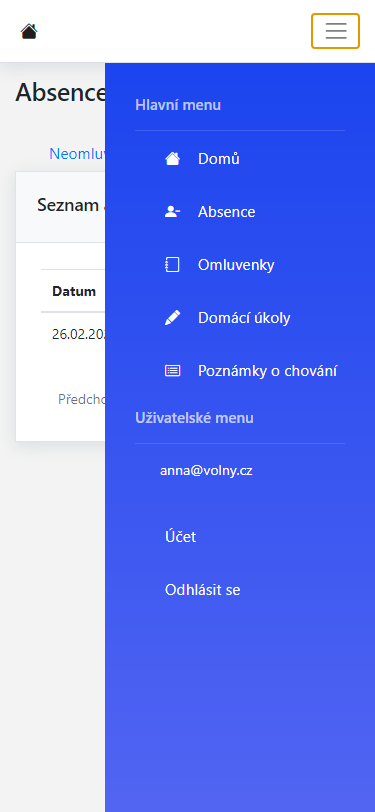
\includegraphics[width=0.5\textwidth]{images/aplikace_responzivni.png}
	\caption{Ukázka responzivního chování}
	\label{app-responz}
\end{figure}


\subsection{Výsledky testování}
Během testování bylo nalezeno několik menších, ale i závažnějších chyb. Menší chyby se týkaly především formulářů pro vyhledávání ve výsledcích, stránkování a responzivity. První závažnější chyba se objevila v administraci systému, kdy se při změně třídního učitele ve vybrané třídě vymazal původní třídní učitel z databáze. Chyba byla způsobena tím, že třídní učitel musel mít v databázi vyplněnou třídu, kterou má na starosti. Při změně třídního učitele tato podmínka nebyla splněna a uživatel byl ze systému vymazán. Další závažnější chyba se týkala opět administrace systému. Tentokrát se chyba objevila při změně rolí u zaměstnanců školy. Pokud se při přidání role \uv{třídní učitel} zapomnělo na vyplnění třídy, kde má uživatel vykonávat třídnické povinnosti, byl uživatel po potvrzení formuláře vymazán z databáze. Tato chyba byla způsobena především neošetřením formuláře na prázdné hodnoty a tím, že třídní učitel musel mít v databázi vyplněnou třídu, kterou má na starosti. Všechny menší i závažné chyby byly v systému opraveny.

\chapter{Zhodnocení vytvořeného systému}
Tato kapitola je věnována zhodnocení vzniklého systému. V první podkapitole jsou zhodnoceny přínosy vytvořeného informačního systému. Dále následuje vyčíslení nákladů spojených na vývoj a provoz systému. V poslední části jsou uvedeny možnosti budoucího rozšíření systému.

\section{Přínosy použití systému}

\subsection{Zlepšení procesů}
Použitím vzniklého informačního systému dojde k zefektivnění dvou zásadních procesů v rámci práce s třídní knihou. Jedná se o proces zápisu informací o proběhnuté hodině a proces omlouvání absence žáků.

U procesu zápisu informací o proběhnuté hodině je největším přínosem fakt, že třídní kniha je vždy přístupná a odpadá tedy její hledání v případě ztráty.

U omlouvání absence žáků je největší výhodou to, že odpadl student jako účastník tohoto procesu. To řeší hned několik problémů. Zaprvé, že student nemůže absenci zatajit a rodič se o ní dozví vždy včas. Zadruhé, že student již nemá téměř žádnou šanci omluvenku zfalšovat, protože omlouvání absence probíhá z účtu rodiče. Jedinou možností je, že by se student dozvěděl heslo, kterým se rodič přihlašuje do systému nebo že by se rodič zapomněl odhlásit. Obě možnosti jsou však problémem rodičů a nedají se z hlediska informačního systému rozumně řešit. Třetí problém, který vyřazení studenta z procesu řeší je ten, že student již nebude moci záměrně zkracovat čas vyučování řešením administrativních záležitostí s třídním učitelem. Nebo naopak, že student nebude muset řešit doručování omluvenek v rámci času určeného na přestávku.

\subsection{Práce odkudkoliv}
Přínosem použití informačního systému je fakt, že lze do systému přistupovat odkudkoliv. To je zvláště přínosné při distanční výuce, kdy zkrátka není možné, aby mělo více učitelů, vyučujících z různých míst, přístup k jedné papírové třídní knize.

Tato výhoda také souvisí s tím, že třídní knihu může používat více uživatelů naráz. Například třídní učitel může řešit omluvenky od rodičů a zároveň učitel může zapsat informace o právě probíhající hodině.

\subsection{Archivace}
Dalším přínosem systému je snadná archivace. Aplikace dokáže vyexportovat třídní knihu do formátu PDF. Poté má škola dvě možnosti, buď soubor vytiskne a bude archivovat v papírové podobě, nebo PDF souboru obstará elektronický podpis nebo elektronické časové razítko a bude archivovat v digitální podobě (na fyzickém nosiči). Archivací v digitální podobě odpadají škole náklady spojené s tiskem a nejsou potřeba velké prostory k uložení. Na druhou stranu je potřeba nakoupit hardware, na kterém budou data uložena.

\subsection{Opravné záznamy}
Opravné zápisy jsou dalším přínosem informačního systému. V případě potřeby, aplikace umožňuje příslušným uživatelům upravit zápis o proběhnuté hodině v třídní knize. Pokud například třídní učitel zjistí při kontrole, že něco není v pořádku, není problém danou chybu opravit.

\section{Náklady na systém}

\subsection{Náklady na vývoj}
Náklady na vývoj se primárně odvíjí od stráveného času nad tvorbou informačního systému. Do výpočtu je zahrnut jak čas na realizaci, tedy implementaci a testování systému, tak i čas strávený nad analýzou a sběrem požadavků, rešerší již existujících aplikací a návrhem systému. V tabulce \ref{tab:development} lze vidět hrubý odhad stráveného času nad jednotlivými částmi.
Zkratka MD znamená \uv{man--day} neboli \uv{člověkoden} a označuje pracovní čas jedné osoby za jeden pracovní den, typicky 8 hodin. \cite{manday}
\clearpage

\begin{table}[h]
    \centering
    \begin{tabular}{|c|c|}
        \hline
         Analýza & 7 MD \\
         \hline
         Rešerše & 5 MD \\
         \hline
         Návrh & 10 MD \\
         \hline
         Implementace & 27 MD \\
         \hline
         Testování & 3 MD \\
         \hline
         \hline
         Celkem & 52 MD = 416 hodin \\
         \hline
    \end{tabular}
    \caption{Odhad času na vývoj systému}
    \label{tab:development}
\end{table}

Cena za vývoj softwaru je podle \cite{md-benchmark} 6 000 Kč/MD. Jedná se o průměrnou cenu kontraktora, který vyvíjí v prostředí .NET, ve třetím kvartálu roku 2020 \cite{md-benchmark}. Po vynásobení průměrné ceny za MD s počtem strávených MD dostáváme částku 312 000 Kč, což je výsledná cena za vývoj. Cena nezahrnuje další výdaje spojené s vývojem, například licence k vývojářským nástrojům a operačnímu systému, koupi počítače, apod.

\subsection{Náklady na zavedení a provoz}
Vzniklý informační systém musí být provozován na serveru, který umí zpracovávat HTTP požadavky. V tomto ohledu má škola několik možností.

\subsubsection*{Sdílený server}
Pronájem sdíleného serveru je nejlevnější možnost pro provoz aplikace. Aplikace je umístěna na server, kde sdílí prostředky (RAM, CPU) s dalšími hostovanými aplikacemi \cite{webhosting-difference}.

Výhodou sdíleného serveru je především cena. Nevýhodou je malá přidělená operační paměť a fakt, že rychlost aplikace mohou ovlivňovat ostatní hostované webové stránky.

Vzhledem k omezeným přiřazeným zdrojům, není tento způsob provozu vzniklé aplikace doporučen.

\subsubsection*{Virtuální privátní server}
V případě virtuálního privátního serveru (VPS) je jeden fyzický server rozdělen na několik virtuálních, které poté poskytovatel pronajímá \cite{webhosting-difference}. Je zde garantována velikost RAM, počet CPU, velikost úložiště, apod.

Jedná se o kompromis mezi sdíleným a dedikovaným serverem, jak z pohledu ceny a výkonu, tak z pohledu kontroly nad serverem.

\subsubsection*{Dedikovaný server}
V tomto případě se jedná o pronájem celého fyzického serveru. Nájemce má správcovský přístup na server a může kontrolovat vše od operačního systému po zabezpečení \cite{webhosting-difference}.

Jelikož se jedná o pronájem celého serveru, cena bude vyšší než u předchozích řešení. Zároveň je pro správu serveru potřeba technická znalost. 

\subsubsection*{Cloud}
V případě cloudu není aplikace provozována pouze na jednom serveru, ale na síti propojených virtuálních a fyzických serverů \cite{what-is-cloud}.

Výhodou je, že nájemce platí jen za ten výkon a úložiště, které skutečně využije. Další výhodou je snadná škálovatelnost aplikace. Nevýhodou je, že výpočet ceny závisí na mnoha faktorech, které se mohou každý měsíc lišit a může se tak lišit i měsíční cena za pronájem \cite{cloud-cons}.

\subsubsection*{Fyzický server}
Poslední možností je pořízení fyzického serveru, který bude škola provozovat sama. 
Výhodou je, že má škola absolutní kontrolu nad provozem aplikace, daty, konfigurací serveru, apod. Nevýhodou jsou náklady na zavedení a provoz. Škola musí zakoupit (v případě, že server již nevlastní) server, případně licence na operační systém a databázi. Nastavení serveru musí provést technik. Další náklady vznikají za spotřebovanou elektřinu, zabezpečení serverovny, apod.

Toto řešení je vhodné především pro technicky zaměřené školy, které již server vlastní, mají vybudované zázemí pro provoz serveru a zaměstnávají technicky zaměřené osoby. Dále je toto řešení vhodné pro velké školy, které jsou ochotné investovat do provozu informačního systému a chtějí mít absolutní kontrolu nad systémem.

\subsubsection{Výběr způsobu provozu}
Výběr provozu aplikace z výše uvedených možností záleží především na velikosti školy, tedy na potřebné velikosti úložiště a potřebném výkonu serveru.

Ve výběru vhodného způsobu provozu byl zohledněn počet uživatelů systému a jejich vliv na úložiště a paměť RAM. Dále byly zohledněny minimální požadavky zvolených technologií na systém. Vzhledem k tomu, že MSSQL databáze požaduje pro operační systém Linux alespoň dvoujádrový procesor \cite{sqlserver-linux-req}, nebylo možné zvolit levnější řešení, i když by to počet uživatelů dovoloval. Vybrané řešení lze vidět v tabulce \ref{tab:service-prices}. Řešení je pro školy s počtem žáků do 250.
\clearpage

\begin{table}[h]
    \centering
    \begin{tabular}{|p{6cm}|c|}
        \hline
         Položka & Cena (bez DPH) \\
         \hline
         \hline
         VPS Large od společnosti FORPSI (INTERNET CZ, a.s.) \cite{linux-server} & 300 Kč/měsíc \\
         \hline
         CZ doména & 149 Kč/rok \\
         \hline
         SSL certifikát & 800 Kč/rok \\
         \hline
         Správa & 5 600 Kč/rok \\
         \hline
         \hline
         Celkem bez správy & 4 549 Kč/rok \\
         \hline
         Celkem se správou & 10 149 Kč/rok \\
         \hline
    \end{tabular}
    \caption{Náklady na provoz informačního systému}
    \label{tab:service-prices}
\end{table}

Správu serveru lze dělat svépomocí (vyžaduje technickou znalost) nebo si zaplatit odborníka. V případě správy serveru třetí stranou se roční rozsah prací odhaduje na 1 MD, což podle \cite{md-benchmark} odpovídá 5 600 Kč.


\subsection{Srovnání s konkurencí}
Vzniklý informační systém nabízí zajímavou alternativu ke komerčním řešením na trhu. Jedná se o open-source systém, kde zákazník platí pouze za provoz aplikace, případně údržbu. Díky rozdělení systému na moduly umožňuje snadné rozšíření o další funkce. V tabulce \ref{tab:prices-comparasion} lze vidět srovnání ročních nákladů aplikací uvedených v rešeršní části se vzniklým informačním systémem (ceny jsou uvedeny pro školy s počtem žáků do 250).

\begin{table}[h]
    \centering
    \begin{tabular}{|c|c|}
        \hline
         Řešení & Cena (bez DPH) \\
         \hline
         \hline
         Vytvořená aplikace v rámci BP (bez správy) & 4 549 Kč/rok \\
         \hline
         Vytvořená aplikace v rámci BP (se správou) & 10 149 Kč/rok \\
         \hline
         Etřídnice & 6 000 Kč/rok \\
         \hline
         Bakaláři & neuvedeno \\
         \hline
         Edookit & 29 636 -- 59 272 Kč/rok \\
         \hline
    \end{tabular}
    \caption{Srovnání ročních nákladů na provoz jednotlivých systémů}
    \label{tab:prices-comparasion}
\end{table}


\section{Možnosti rozšíření}
Vzniklý informační systém obsahuje základní funkcionalitu pro správu třídních knih. Díky návrhu architektury pro snadnou rozšiřitelnost však může v budoucnu řešit další problémy spojené se školní agendou.

Následující návrhy nových modulů mohou představovat zajímavé možnosti dalšího rozšíření.

\subsubsection*{Žákovská knížka}
Tento modul by sloužil k přehledu známek, které studenti dostávají. Ke známkám by měli přístup učitelé, rodiče i žáci. Rodiče by tak byli vždy informování o klasifikaci svých dětí.

\subsubsection*{Platby}
Modul platby by sloužil pro veškeré úhrady spojené se studiem dětí. Rodiče by měli možnost platit tímto způsobem například sportovní kurzy, výlety, příspěvky škole, apod. Odpadla by nutnost řešit tyto záležitosti na třídních schůzkách, přes e-mail či prostřednictvím žáka.

\subsubsection*{Rozvrhy}
Tento modul by sloužil pro tvorbu a zobrazení rozvrhu dané třídy. Žáci a rodiče by byli vždy informováni o probíhaných hodinách, změnách v rozvrhu, apod. Tento modul by také mohl sloužit pro správu tématických okruhů. Učitelé by si tak při zápisu do třídní knihy mohli místo psaní tématu dané hodiny pouze vybrat ze seznamu okruhů.

\subsubsection*{}
Rozšíření o nový modul se provede vytvořením nového projektu v aplikační vrstvě, vytvořením nového repository v datové vrstvě a vytvořením nové oblasti v prezentační vrstvě. Dále je nutné přidat odkaz do hlavního navigačního menu, který bude sloužit pro přechod do nového modulu. Po přidání modulu je nutné aplikaci znovu publikovat (připravit na nasazení).




\begin{conclusion}
Cílem této práce bylo navrhnout a implementovat informační systém, který podporuje správu třídních knih. Tvorba systému měla být v souladu s metodami softwarového inženýrství a měla zahrnovat analýzu problémové domény, rešerši existujících řešení, návrh systému, implementaci a testování, zhodnocení přínosů použití systému a odhadnutí nákladů na zavedení a provoz.

Vývoj aplikace začal analýzou problémové domény, kde hlavním výstupem je stanovení funkčních a nefunkčních požadavků na systém. Ty se podařilo sestavit na základě konzultace s učitelkou vyučující na základní škole. V analýze byly také identifikovány klíčové procesy, které byly namodelovány jak s použitím informačního systému, tak bez něj, a vytvořen doménový model, který popisuje jednotlivé entity v problémové doméně a pomáhá pochopit vztahy mezi nimi.

Následovala stručná rešerše, kde byly popsány již existující řešení elektronizace třídních knih. Na konci bylo provedeno shrnutí kladů a záporů jednotlivých systémů.

Návrh je věnován architektuře systému, případům užití a tvorbě základního uživatelského rozhraní aplikace. Systém je postaven na třívrstvé architektuře, která rozděluje aplikaci na prezentační, aplikační a datovou vrstvu. Pro další strukturování zdrojového kódu je v prezentační vrstvě použit návrhový vzor MVC. Jednotlivé funkční celky jsou rozděleny do samostatných modulů, což usnadňuje budoucí vývoj. Případy užití, které představují průchody aplikací, byly sestaveny na základě stanovených požadavků.

Výsledný systém má podobu webové aplikace a je vytvořen na platformě .NET Core, která je požadována v zadání práce. Pro vývoj byl použit framework ASP.NET Core MVC, který je určen pro tvorbu webových aplikací. Pro práci s databází byl použit Entity Framework Core, který umožňuje pracovat s tabulkami databáze jako s objekty. Vzhled uživatelského rozhraní byl tvořen za pomoci frameworku Bootstrap. Aplikace byla řádně otestována pomocí testovacích scénářů vycházejících z případů užití.
\newline

Po dokončení implementace a testování byly zhodnoceny přínosy použití systému a byly odhadnuty náklady na zavedení a provoz. Použití systému umožňuje práci odkudkoliv, což pomáhá řešit administrativní zátěž dálkové výuky, zjednodušuje archivaci třídních knih či zefektivňuje identifikované procesy. Odhad nákladů ukázal, že výsledný systém může mít pro školy zajímavé provozní náklady, avšak započítá-li se podpora aplikace, nemusí se jednat o nejlevnější řešení. 

Všechny stanovené cíle se podařilo úspěšně splnit, systém je připraven k případnému provozu a díky tomu, že je vyvíjen jako open-source projekt, může vývoj dalších funkcionalit probíhat nezávisle na autorovi práce.
\end{conclusion}


\emergencystretch=1em
\printbibliography

\appendix

\chapter{Seznam použitých zkratek}
% \printglossaries
\begin{description}
	\item[UML] Unified Modeling Language
	\item[GDPR] General Data Protection Regulation
	\item[DPH] Daň z přidané hodnoty
	\item[PDF] Portable Document Format
	\item[MVC] Model-view-controller
	\item[HTML] Hypertext Markup Language
	\item[CSS] Cascading Style Sheets
	\item[IoT] Internet of Things
	\item[IoC] Inversion of Control
	\item[URL] Uniform Resource Locator
	\item[ORM] Object Relational Mapping
	\item[LINQ] Language Integrated Query
	\item[SQL] Structured Query Language
	\item[MD] Man-day
	\item[VPS] Virtual Private Server
\end{description}

\chapter{Diagramy}
\begin{figure}[h]
\begin{center}
	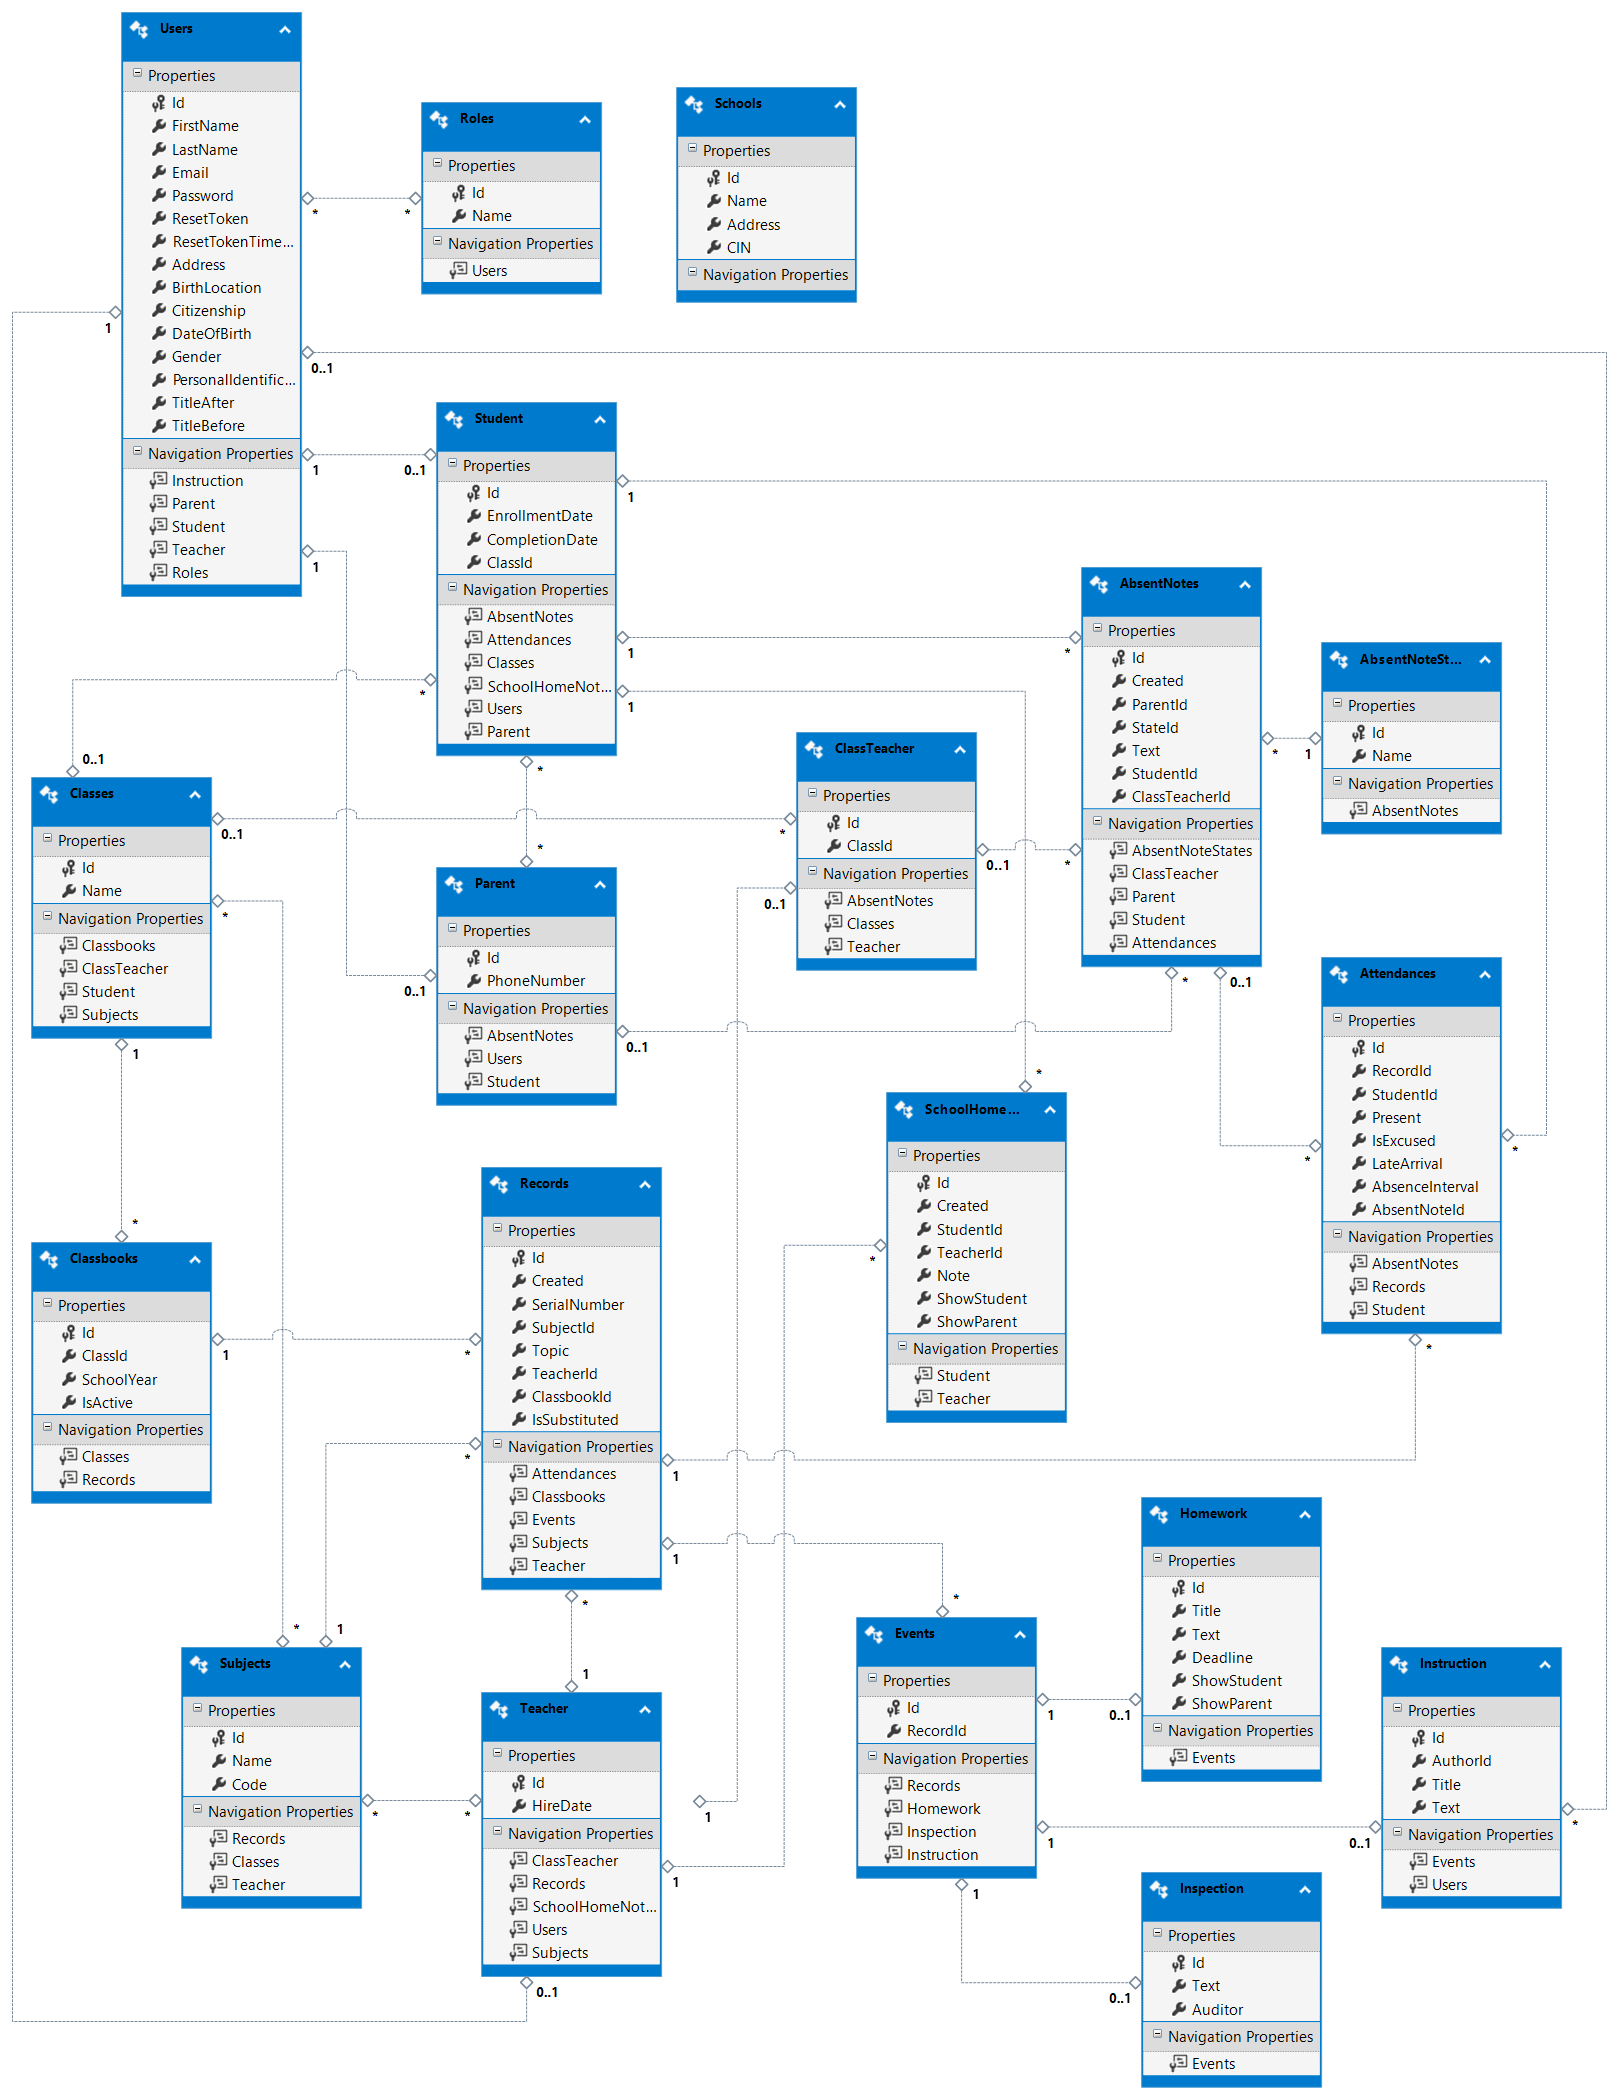
\includegraphics[width=1.14\textwidth]{images/db.png}
	\caption{Schéma databáze}
	\label{db-diagram}
\end{center}
\end{figure}    


\chapter{Ukázky aplikace}

\begin{figure}[h]
	\centering
	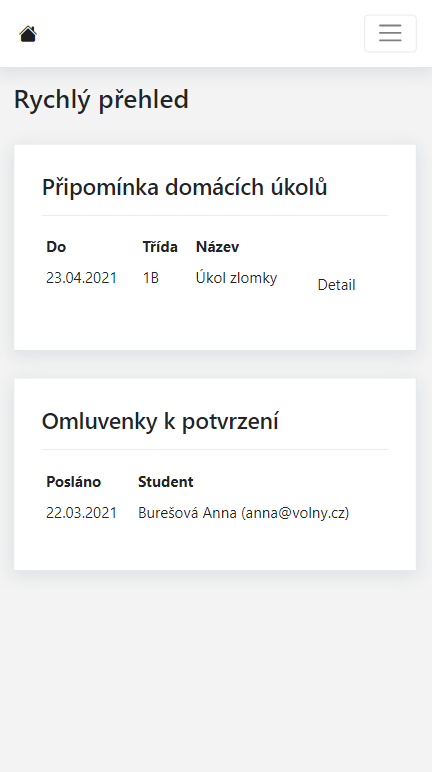
\includegraphics[width=0.5\textwidth]{images/app_samples/ucitel-rychly-prehled-responzivni.png}
	\caption{Stránka s rychlým přehledem pro učitele (responzivní)}
	\label{ucitel-rychly-prehled-responzivni}
\end{figure}
\clearpage

\begin{sidewaysfigure}[h]
	\centering
	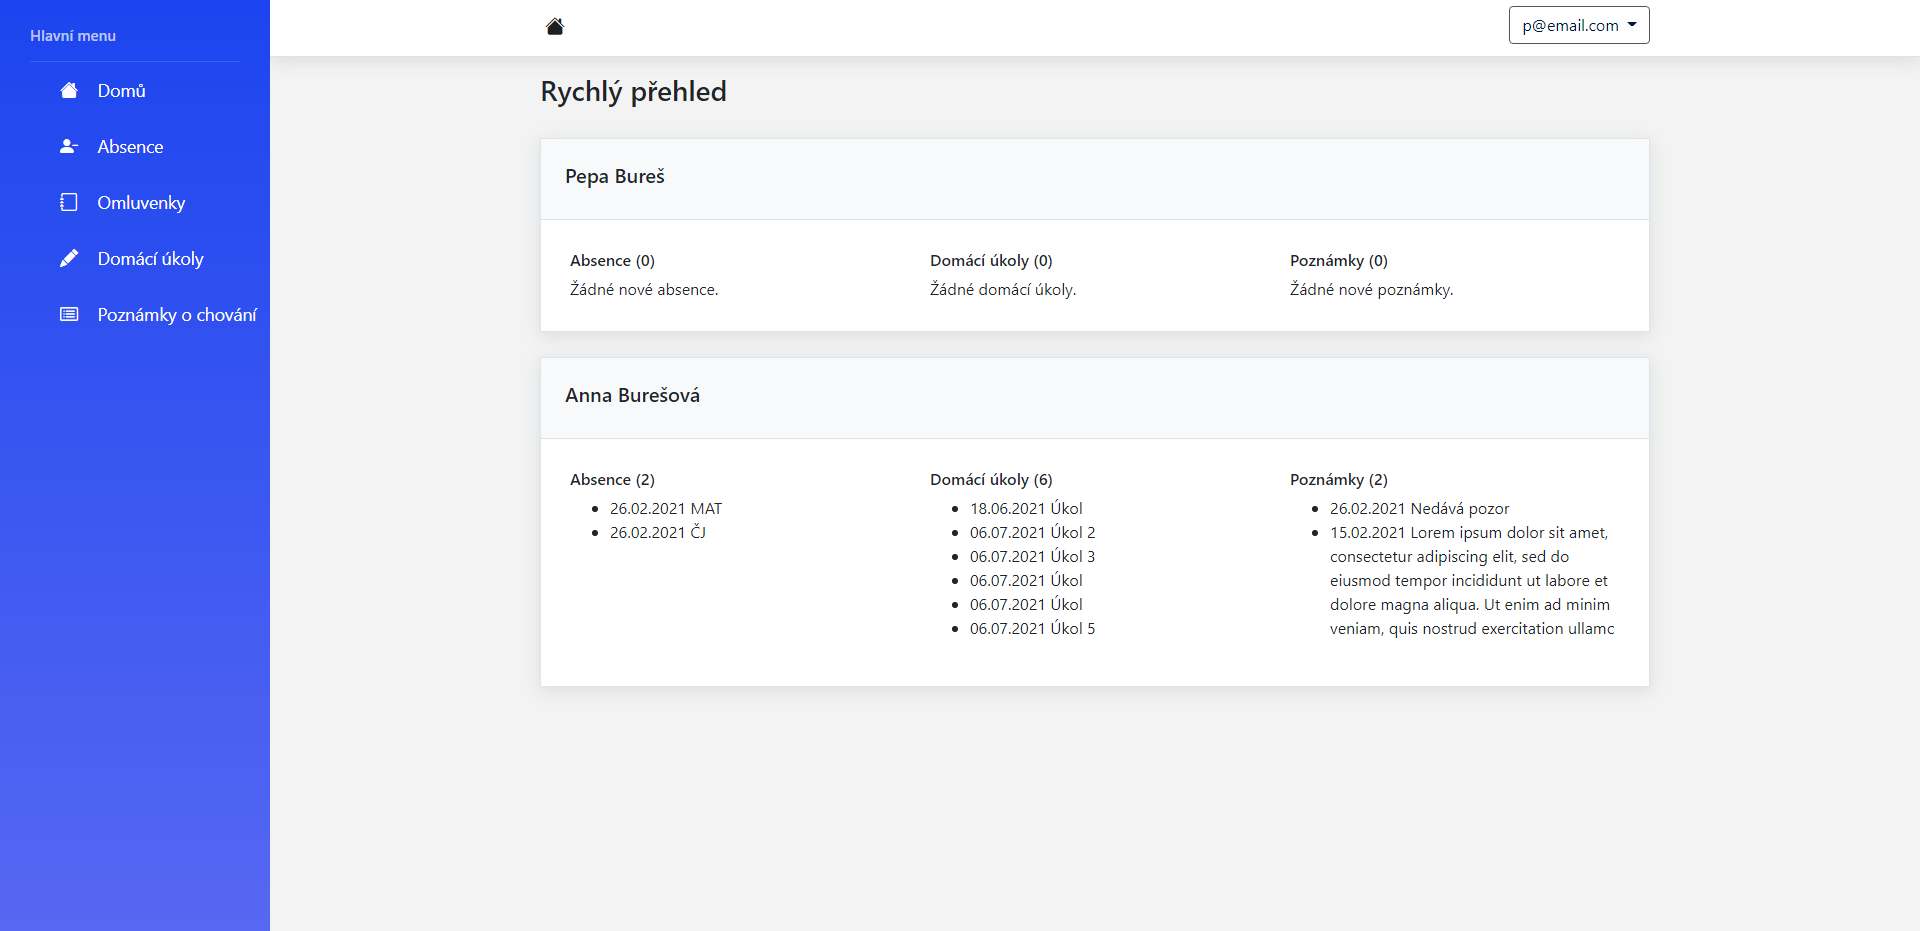
\includegraphics[width=\textwidth]{images/app_samples/rodic-rychly-prehled.png}
	\caption{Stránka s rychlým přehledem pro rodiče}
	\label{rodic-rychly-prehled}
\end{sidewaysfigure}
\clearpage

\begin{sidewaysfigure}[h]
	\centering
	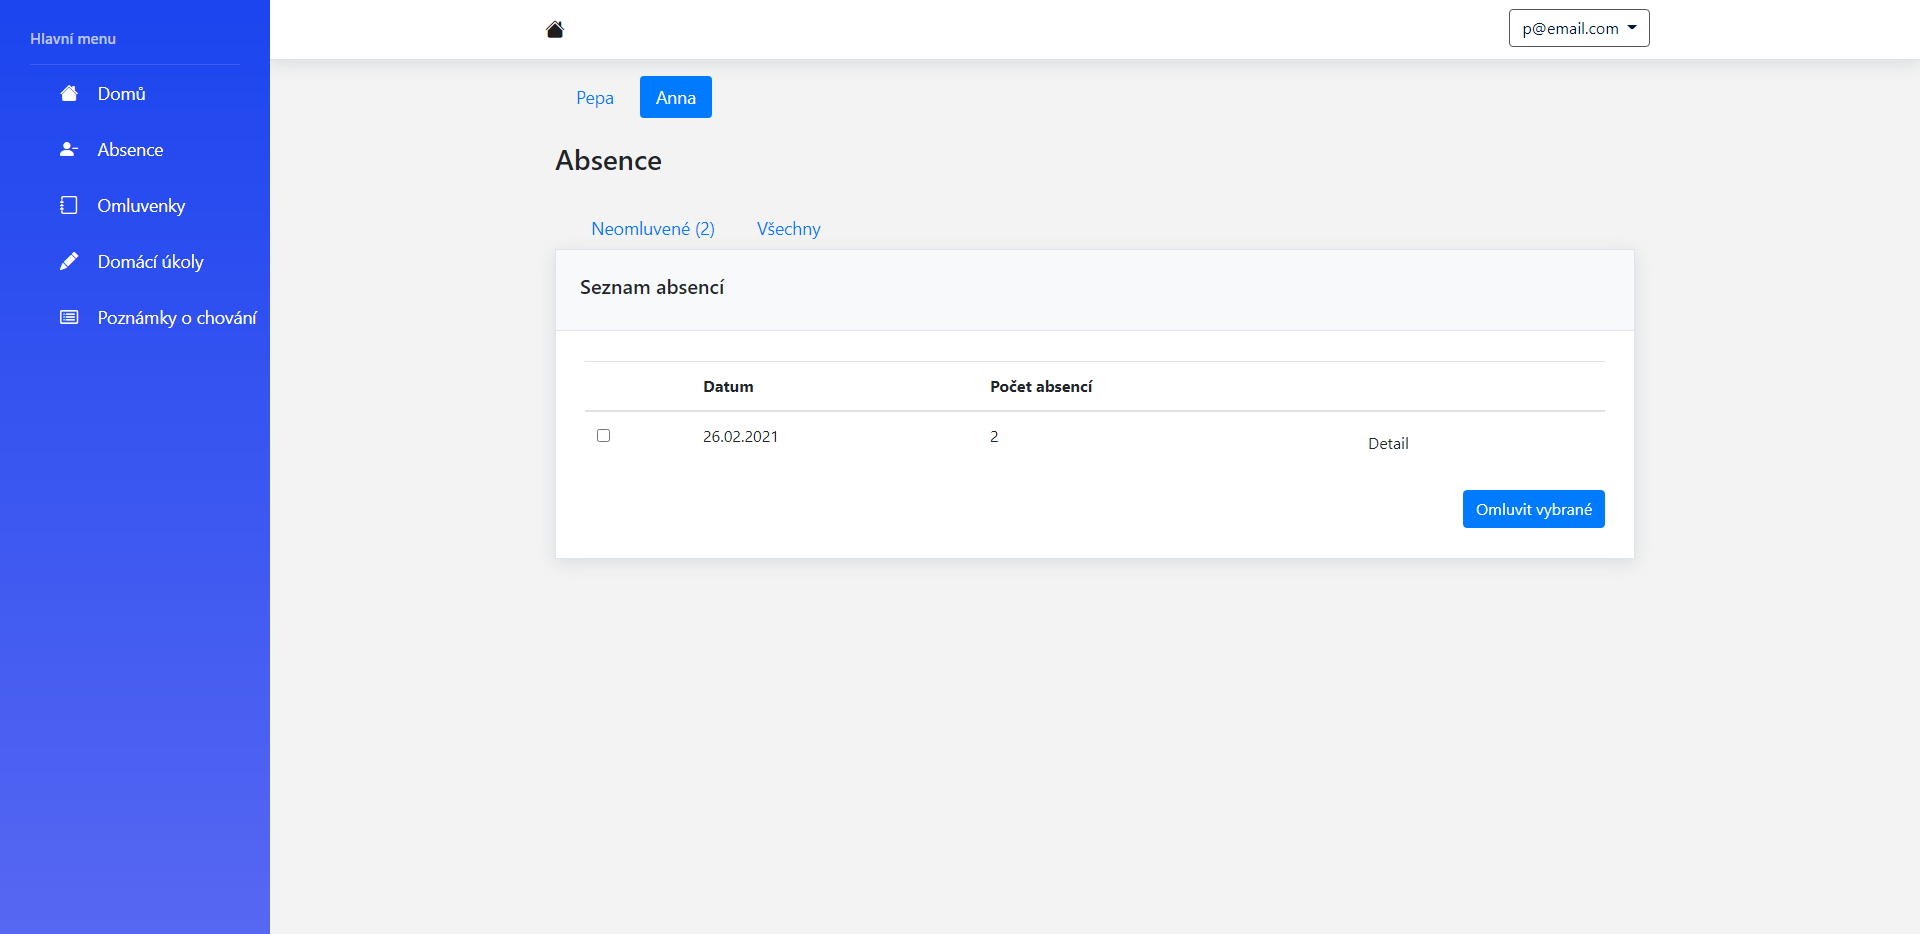
\includegraphics[width=\textwidth]{images/app_samples/rodic-absence.png}
	\caption{Stránka zobrazující absence žáka jeho rodičovi}
	\label{rodic-absence}
\end{sidewaysfigure}
\clearpage

\begin{sidewaysfigure}[h]
	\centering
	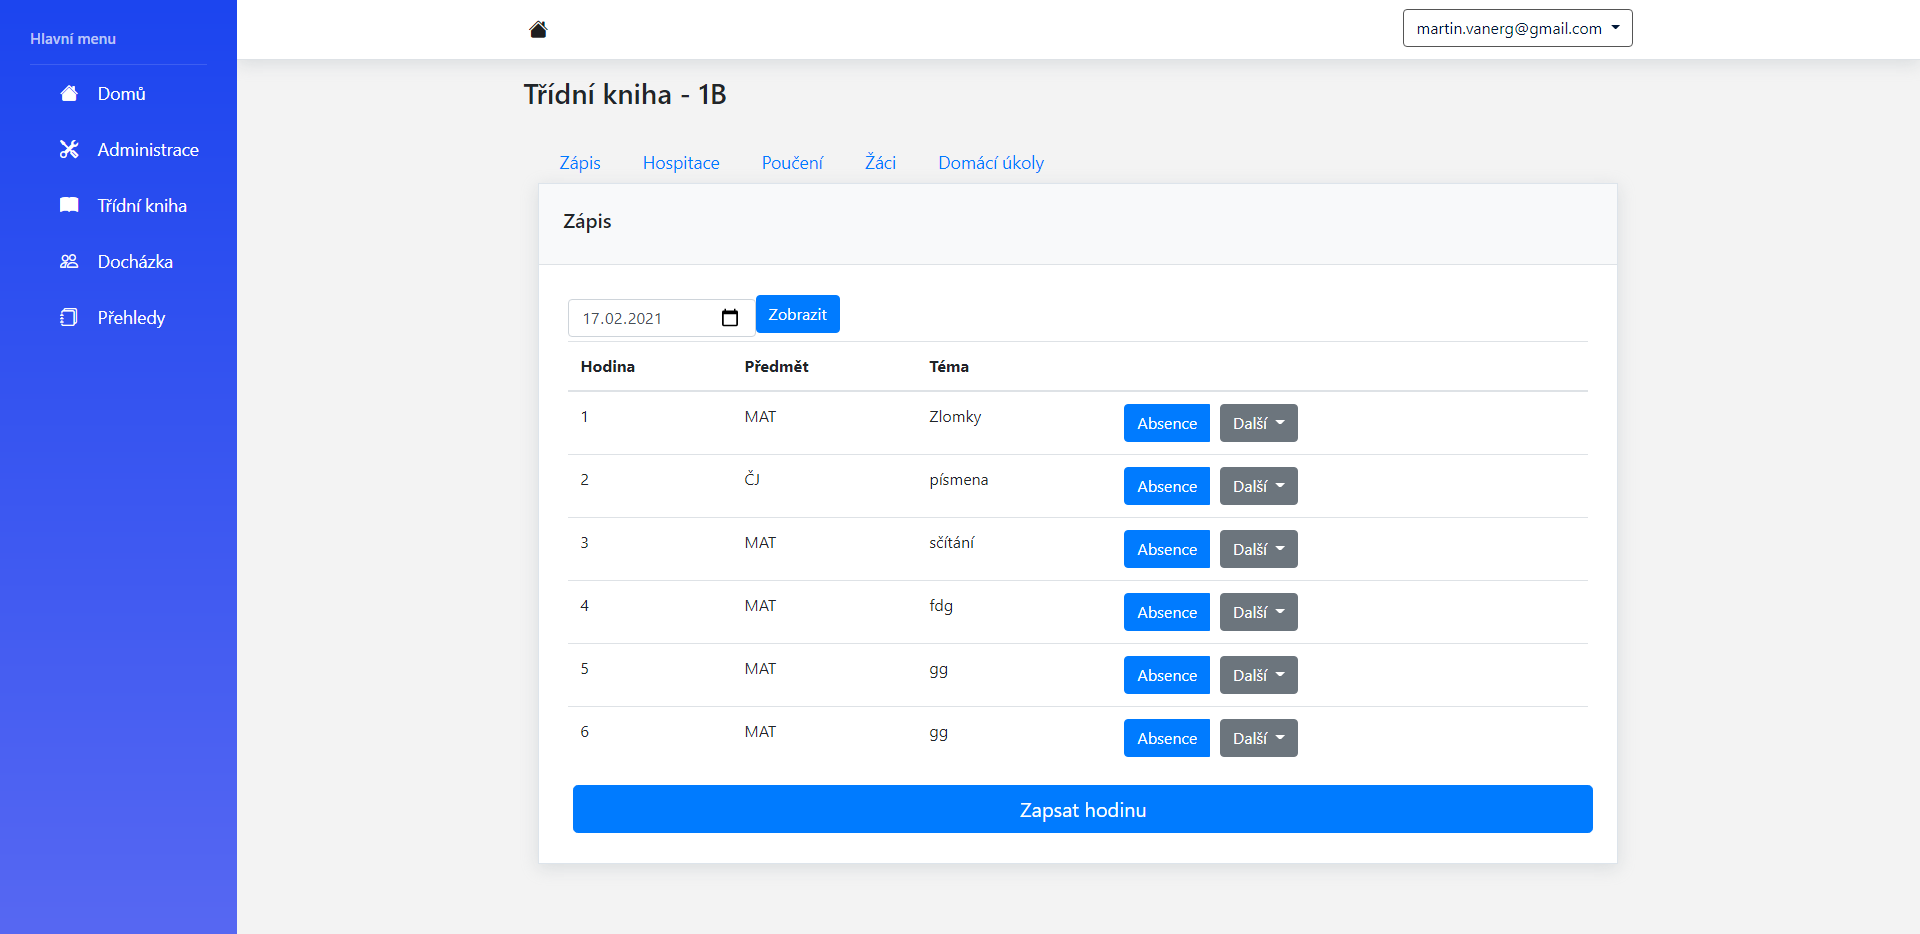
\includegraphics[width=\textwidth]{images/app_samples/tridni-kniha-otevrena-data.png}
	\caption{Otevřená třídní kniha}
	\label{tridni-kniha-otevrena}
\end{sidewaysfigure}
\clearpage

\begin{sidewaysfigure}[h]
	\centering
	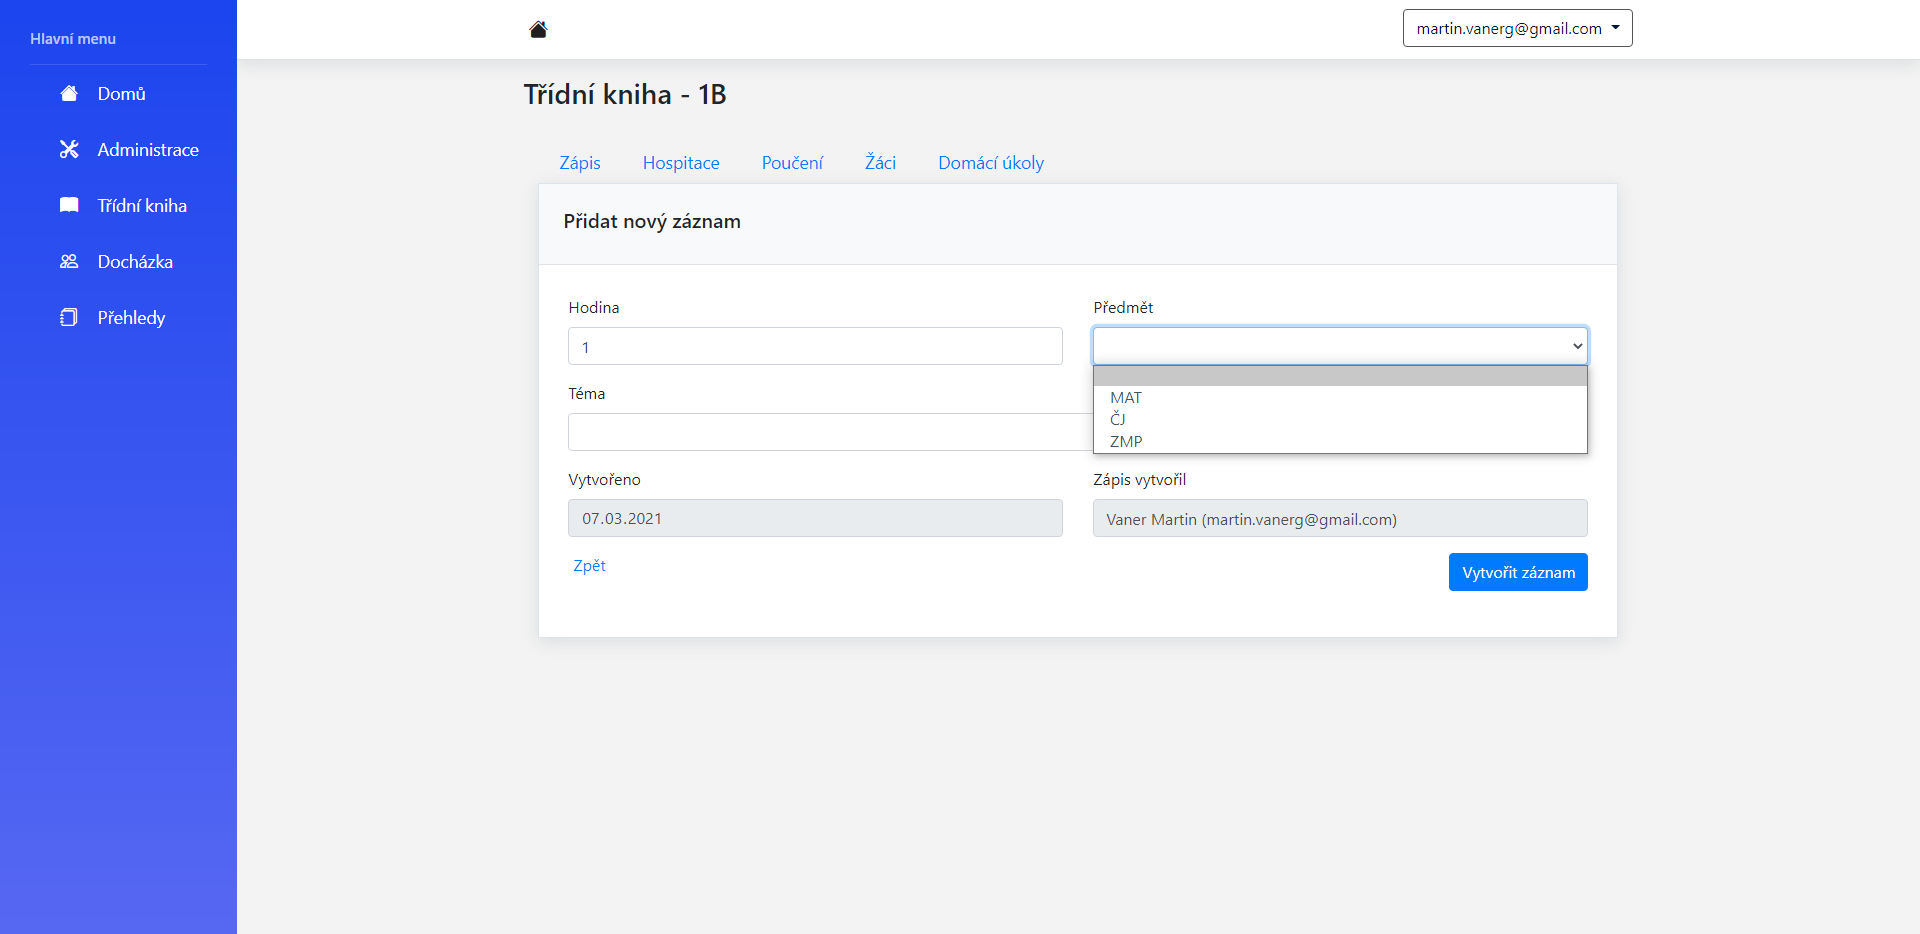
\includegraphics[width=\textwidth]{images/app_samples/tridni-kniha-zapis.png}
	\caption{Formulář pro zápis do třídní knihy}
	\label{tridni-kniha-zapis}
\end{sidewaysfigure}
\clearpage

\begin{sidewaysfigure}[h]
	\centering
	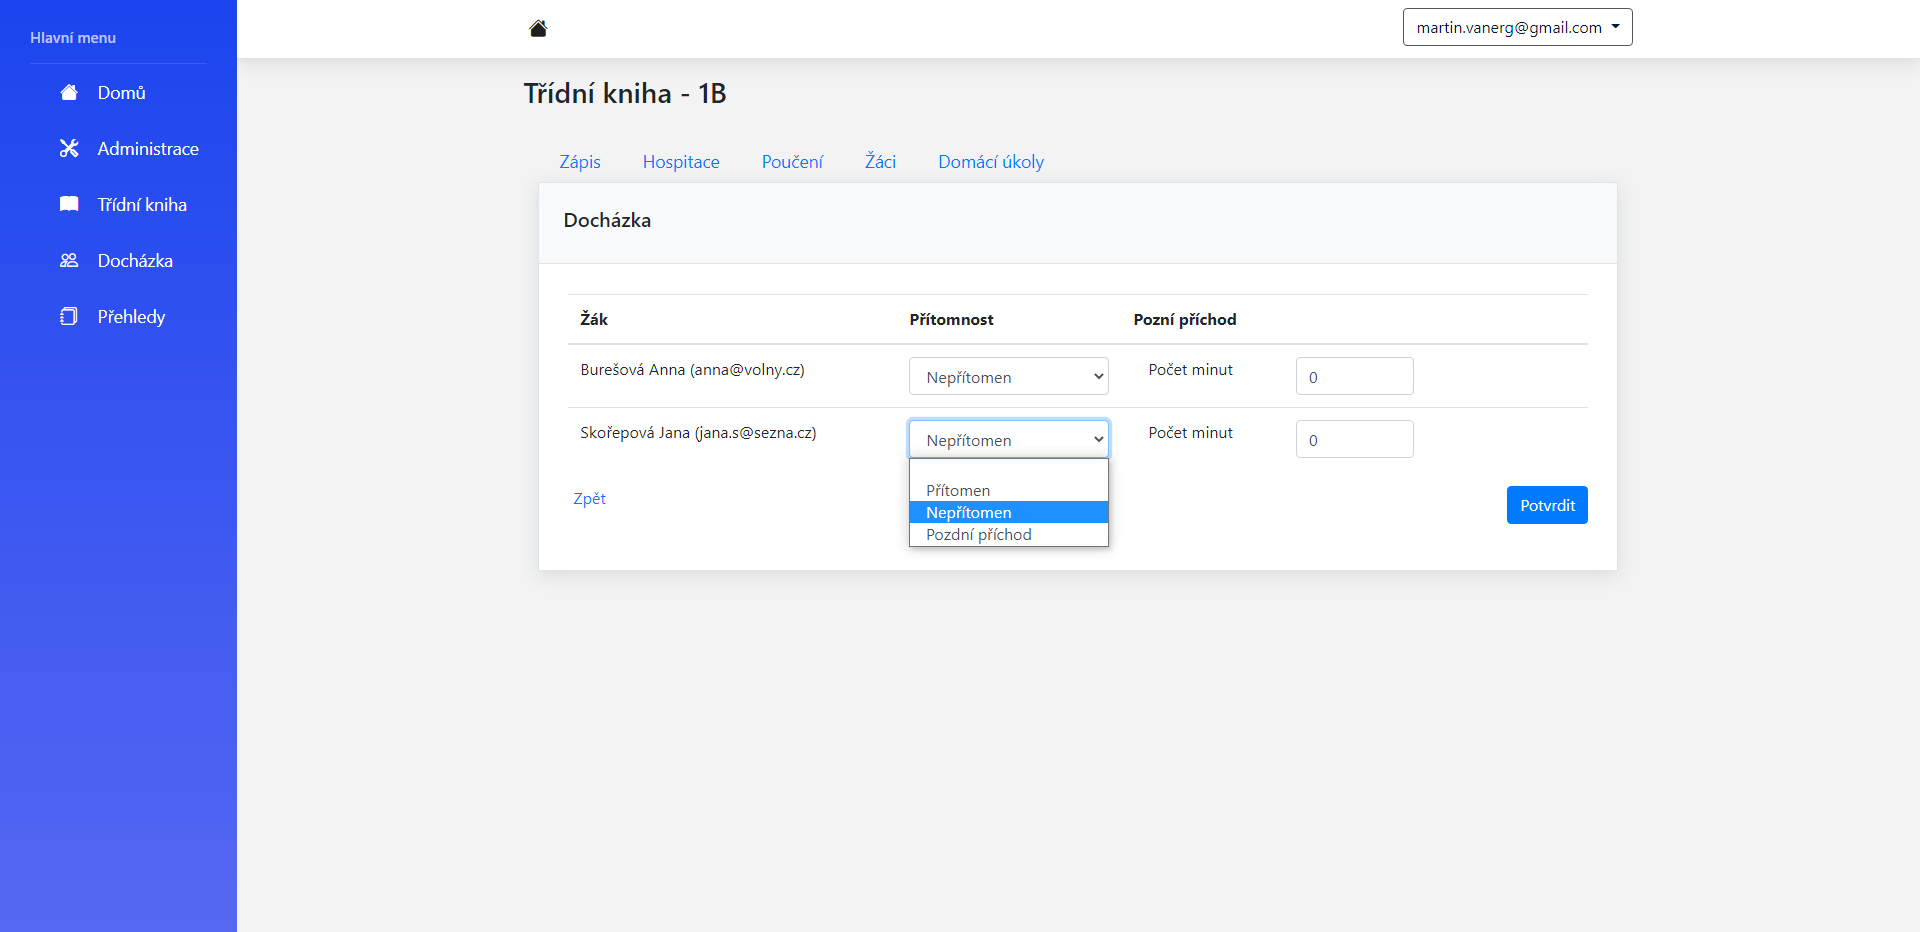
\includegraphics[width=\textwidth]{images/app_samples/tridni-kniha-absence.png}
	\caption{Formulář pro vyplnění absence}
	\label{tridni-kniha-absence}
\end{sidewaysfigure}

\chapter{Obsah přiložené SD karty}


\begin{figure}
	\dirtree{%
		.1 readme.md\DTcomment{stručný popis obsahu SD karty}.
		.1 publish \DTcomment{adresář s verzemi aplikace}.
		.2 MSSQL \DTcomment{verze aplikace pro Microsoft SQL Server databázi}.
		.2 PostgreSQL \DTcomment{verze aplikace pro PostgreSQL databázi}.
		.2 deployment.pdf \DTcomment{instalační příručka}.
		.1 ElectronicClassbook \DTcomment{zdrojové kódy implementace}.
		.1 thesis\DTcomment{text práce}.
		.2 src \DTcomment{zdrojová forma práce ve formátu \LaTeX{}}.
		.2 BP\_Vaner\_Martin\_2021.pdf\DTcomment{text práce ve formátu PDF}.
		.2 assignment.pdf\DTcomment{zadání práce ve formátu PDF}.
		.1 samples \DTcomment{ukázky aplikace}.
		.2 screenshots \DTcomment{obrazové ukázky aplikace}.
		.2 video.mp4 \DTcomment{komentovaná video ukázka aplikace}.
	}
\end{figure}

\end{document}
